\documentclass{report}
\usepackage{graphicx}
\usepackage[spanish]{babel}
\usepackage[utf8]{inputenc} % Ensures proper handling of special characters
\usepackage{amsthm}
\usepackage{amsmath}
\usepackage{amsfonts}
\usepackage{hyperref}
\usepackage{mathrsfs}
\usepackage{tikz}
\usepackage[font=footnotesize,labelfont=bf,labelsep=colon]{caption} % Personalización de captions
\DeclareMathOperator*{\argmin}{arg\,min}
% Define the unnumbered theorem
\newtheorem{thm}{Teorema}[section]
\newtheorem{lem}{Lema}[section]
\newtheorem{prop}{Proposición}[section]
\newtheorem{cor}{Corolario}[thm]
\newtheorem{dfn}{Definición}[section]
\newtheorem{obs}{Observación}[section]
\newtheorem{ej}{Ejemplo}[section]

%\newtheorem*{def}{Definicion}

\begin{document}


\title{Fundamentos Matemáticos \\ del Aprendizaje Automático}
\author{Nicolas Silva Nash \\ Departamento de Matemática \\ Universidad Nacional del Comahue}
%\date{\today}
\maketitle
\tableofcontents
\chapter{Resultados Preliminares}
\section{Medida}

\begin{dfn}
    Llamamos \textit{espacio muestral} a un conjunto $\Omega$ de posibles resultados de un experimento aleatorio.
\end{dfn}
\begin{dfn}
Una familia de subconjuntos de un espacio muestral $S=\{A: A\subseteq\Omega\}$,  se llama una $\sigma$-\emph{álgebra}, si satisface las siguientes tres propiedades:

\begin{enumerate}
    \item \( \Omega \in S \).
    \item Si \( A \in S \), entonces \( A^c \in S \) (cerradura bajo complemento).
    \item Si \( A_1, A_2, \ldots \in S \), entonces \( \bigcup_{i=1}^\infty A_i \in S \) (cerradura bajo uniones numerables).
\end{enumerate}
\end{dfn}

\begin{obs}
    Diremos que un conjunto a lo sumo numerable es numerable. Es decir, un conjunto numerable será para nosotros un conjunto
    para el que puede definirse una correspondencia biyectiva con un subconjunto (no necesariamente estricto) de los números naturales.
\end{obs}

\begin{dfn}
Sea \( \mu \) una función definida sobre una \(\sigma\)-álgebra \( S \). Diremos que \( \mu \) es una \textit{medida} sobre \( S \) si se cumple:

\begin{enumerate}
  \item \( 0 \leq \mu(E) \leq +\infty \), para todo \( E \in S \),
  \item \( \mu\left( \displaystyle\bigcup_k E_k \right) = \displaystyle\sum_k \mu(E_k) \) para toda familia numerable \( \{E_k\} \) de conjuntos disjuntos en \( S \).
\end{enumerate}
\end{dfn}

\begin{dfn}
Sea

\[
I = \left\{ x \in \mathbb{R}^n : a_j \leq x_j \leq b_j, \quad j = 1, \dots, n \right\},
\]
un conjunto de intervalos cerrados \( n \)-dimensionales. Definimos su \emph{volumen} como

\[
v(I) = \prod_{j=1}^{n} (b_j - a_j).
\]
\end{dfn}

\begin{dfn}
Sea \( E \subseteq \mathbb{R}^n \). Se cubre \( E \) mediante una colección numerable \( \mathcal{S} = \{ I_k \} \) 
de intervalos \( n \)-dimensionales cerrados. Sea:

\[
\sigma(\mathcal{S}) = \sum_{k} v(I_k).
\]
Entonces, definimos la \textit{medida exterior de Lebesgue} del conjunto \( E  \) como:

\begin{equation*}
|E|_e = \inf \sigma(\mathcal{S}),
\end{equation*}
donde el ínfimo lo tomamos sobre todos los cubrimientos $S$ de $E$.
\end{dfn}

\begin{prop}
    Sea \( E \subseteq \mathbb{R}^n \), entonces:
    \begin{equation*}
        0 \leq \mid E \mid_e \leq +\infty.
    \end{equation*}
\end{prop}

\begin{prop}
    Sea $I$ un intervalo en $R^n$. Entonces, $\mid I \mid_e = v(I)$.
\end{prop}


\begin{dfn}
Un subconjunto \( E \subseteq \mathbb{R}^n \) se dice \textit{medible de Lebesgue} (o simplemente \textit{medible}) si, dado \( \varepsilon > 0 \), 
existe un conjunto abierto \( G \subseteq \mathbb{R}^n \) tal que

\[
E \subseteq G \quad \text{y} \quad |G \setminus E|_e < \varepsilon,
\]

donde \( | \cdot |_e \) denota la medida exterior de Lebesgue.
\end{dfn}

\begin{dfn}
Si \( E \subseteq \mathbb{R}^n \) es un conjunto medible de Lebesgue, entonces su \textit{medida exterior} coincide con su \textit{medida de Lebesgue}, 
que denotamos simplemente por \( \mathscr{L}(E) \). Es decir,
\[
\mathscr{L}(E)  = |E|_e, \quad \text{si } E \text{ es medible}.
\]
\end{dfn}

\begin{thm}
La colección de subconjuntos medibles de Lebesgue de \( \mathbb{R}^n \) forma una \( \sigma \)-álgebra.
\end{thm}


\begin{ej}[Espacio de medida de Lebesgue]
Si \( \mathscr{L}\) es la medida de Lebesgue y \( \Sigma \) es la \(\sigma\)-álgebra de conjuntos medibles de Lebesgue sobre \( \mathbb{R}^n \), 
entonces el triplete \( (\mathbb{R}^n, \Sigma, \mathscr{L}) \) constituye un \textit{espacio de medida}.
\end{ej}

\begin{ej}[Espacio de medida discreto]
Sea \( \mathcal{S} = \{x_k\} \) un conjunto numerable, y sea \( \{a_k\} \) una sucesión de números no negativos. 
Definimos \( \sigma \) como la familia de todos los subconjuntos de \( \mathcal{S} \), y la medida \( \delta \) por:

\[
\delta(E) = \sum_{X_k \in E} a_k.
\]

Entonces, \( (\mathcal{S}, \sigma, \delta) \) es un espacio de medida al que llamamos \emph{discreto}.
\end{ej}

\begin{dfn}
Sea \( \Sigma \) una \( \sigma \)-álgebra de subconjuntos medibles con respecto a una medida $\mu$, de un conjunto dado \( \Omega \). 
Una \emph{función de conjuntos} es una aplicación \( F: \Sigma \to \mathbb{R} \) que satisface las siguientes condiciones:
\begin{enumerate}
    \item \( F(E) \) es finito para todo \( E \in \Sigma \).
    \item \( F \) es \(\sigma\)-aditiva: si \( E = \bigcup_k E_k \), donde \( \{E_k\} \subset \Sigma \) es una familia de conjuntos disjuntos dos a dos, entonces
    \[
        F(E) = \sum_k F(E_k).
    \]
\end{enumerate}
\end{dfn}

\begin{dfn}
Una función de conjuntos \( F \) se dice \emph{absolutamente continua con respecto a la medida de Lebesgue} (o simplemente \emph{absolutamente continua})
 si \( F(E) \to 0 \) cuando la medida de \( E \) tiende a cero. Es decir, \( F \) es absolutamente continua si, dado \( \varepsilon > 0 \), existe \( \delta > 0 \) tal que
\[
\mathcal{L}(F(E)) < \varepsilon \quad \text{siempre que} \quad \mu(E) < \delta.
\]
\end{dfn}


%A los alcances de la primer capítulo, donde nos limitaremos a una descripción intuitiva de la Teoría del Aprendizaje Estadístico, la siguiente
%definición de probabilidad será suficiente. Luego la definiremos de manera más formal, haciendo uso de resultados conocidos de Teoría de la Medida. 
\section{Espacios de Probabilidad}

\begin{dfn}
Dado un espacio muestral \( \Omega \) y una $\sigma$-álgebra asociada \( S \), 
una \emph{función de probabilidad} es una función \( P \colon S \to [0,1] \) que satisface:

\begin{enumerate}
    \item \( P(A) \geq 0 \) para todo \( A \in S \).
    \item \( P(\Omega) = 1 \).
    \item Si \( A_1, A_2, \dots \in S \) son disjuntos por pares, entonces
    \[
        P\left( \bigcup_{i=1}^{\infty} A_i \right) = \sum_{i=1}^{\infty} P(A_i).
    \]
\end{enumerate}
\end{dfn}

\begin{lem}
    Toda función de probabilidad es una medida sobre el espacio $\Omega$, por lo que $(\Omega, S, P)$ conforman un espacio de medida.
\end{lem}

\begin{obs}
    Bajo las condiciones descritas, decimos que $(\Omega, S, P)$ es un \emph{espacio de probabilidad}. Es posible también definir
    a un espacio de probabilidad como un espacio de medida, tal que la medida de todo el espacio es $1$.
\end{obs}

\begin{dfn}
Diremos que una sucesión de conjuntos $\{A_i\}_{i\in\mathbb{N}}$ \emph{crece} al conjunto $A$, y notamos
$$
\{A_i\}_{i\in\mathbb{N}}\nearrow A
$$
si
\begin{enumerate}
    \item $A_1 \subseteq A_2 \subseteq A_3 \subseteq \dots$
    \item $A_i \rightarrow A$ cuando $i\rightarrow \infty$
\end{enumerate}
\end{dfn}

\begin{dfn}
Análogamente, diremos que una sucesión de conjuntos $\{A_i\}_{i\in\mathbb{N}}$ \emph{decrece} al conjunto $A$, y notamos
$$
\{A_i\}_{i\in\mathbb{N}}\searrow A
$$
si
\begin{enumerate}
    \item $\ldots \subseteq A_3 \subseteq A_2 \subseteq A_1 $
    \item $A_i \rightarrow A$ cuando $i\rightarrow \infty$
\end{enumerate}
\end{dfn}

\begin{thm}
Sea \( P \) una función de probabilidad, $A$, $B$ subconjuntos de \(S\), y $\{A_i\}_{i\in\mathbb{N}}$ una familia de conjuntos en $S$. 
Entonces se cumple que:

\begin{enumerate}
    \item \( P(\emptyset) = 0 \), donde \( \emptyset \) es el conjunto vacío.
    \item \( P(A) \leq 1 \).
    \item \( P(A^c) = 1 - P(A) \).
    \item \( P(B \cap A^c) = P(B) - P(A \cap B) \);
    \item \( P(A \cup B) = P(A) + P(B) - P(A \cap B) \);
    \item Si \( A \subseteq B \), entonces \( P(A) \leq P(B) \).
    \item $P\left(\bigcup_{n\in\mathbb{N}}A_n\right) \leq \sum_{n\in\mathbb{N}}P(A_n)$.
    \item Si $\{A_i\}_{i\in\mathbb{N}}\nearrow A$, entonces $P(A_i)\rightarrow P(A)$ cuando $n\rightarrow \infty$.
    \item Si $\{A_i\}_{i\in\mathbb{N}}\searrow A$, entonces $P(A_i)\rightarrow P(A)$ cuando $n\rightarrow \infty$.
\end{enumerate}
\end{thm}

\begin{lem}[Primer Lema de Borel-Cantelli] \label{primer lema de Borel-Cantelli}
Sea \( \{A_n\} \) una sucesión de eventos tales que \( \sum_{n \geq 1} \mathbb{P}(A_n) < \infty \), entonces
\[
\mathbb{P} \left( \limsup_{n \to \infty} A_n \right) = 0.
\]
\end{lem}

\begin{lem}[Segundo Lema de Borel-Cantelli] \label{segundo  lema de Borel-Cantelli}
Sea \( \{A_n\} \) una sucesión de eventos tales que \( \sum_{n \geq 1} \mathbb{P}(A_n) = \infty \) y \( \{A_n\} \) son independientes, entonces
\[
\mathbb{P} \left( \limsup_{n \to \infty} A_n \right) = 1.
\]
\end{lem}


\begin{dfn}
Sea \( (\Omega, S, P) \) un espacio de probabilidad y sean \( A \) y \( B \) dos sucesos, con \( P(B) > 0 \). 
Se define la probabilidad de \( A \) condicionada a \( B \) mediante la expresión,
\[
P(A \mid B) = \frac{P(A \cap B)}{P(B)}.
\]
\end{dfn}

\begin{dfn}
Sean $A, B\in S$, sucesos. Diremos que $A$ y $B$ son \emph{independientes} entre sí si:
$$
P(A\cap B) = P(A)P(B)
$$
\end{dfn}

\begin{obs}
    Notemos que si los sucesos $A$ y $B$ son independientes entre sí, entonces:
    \[
    \begin{split}
        P(A \mid B) =  \frac{P(A \cap B)}{P(B)} =\frac{P(A)P(B)}{P(B)} = P(A),\\
        P(B \mid A) =  \frac{P(B \cap A)}{P(A)} =\frac{P(B)P(A)}{P(A)} = P(B).
    \end{split}
    \]
\end{obs}

\begin{dfn}
Sean $\{A_1, \ldots, A_n\}\in S$, una familia finita de sucesos. Diremos que son \emph{mutuamente independientes} entre sí si:
$$
P\left(\bigcap_{i=1}^n A_i \right) = \prod_{i=1}^{n} P(A_i)
$$
\end{dfn}

\begin{dfn}
Sean $\{A_i\}_{i\in\mathbb{N}}\in S$, una familia infinita numerable de sucesos. En este caso, diremos que los eventos son mutuamente
independientes entre sí si cualquier subcolección finita de la familia lo es.
\end{dfn}

\begin{thm}(\textbf{Bayes})
Sean $A$ y $B$ sucesos en $S$. Entonces
\begin{equation*}
    P(A\mid B) = \frac{P(B\mid A)P(A)}{P(B)}
\end{equation*}
\end{thm}

\section{Variables Aleatorias}

\begin{dfn}
    Llamamos $\sigma$-álgebra de Borel, $\mathcal{B}$, a la menor de todas las $\sigma$-álgebras en $\mathbb{R}$ que contienen a todos los intervalos
    abiertos de números reales. Llamamos \emph{borelianos} a los elementos de $\mathcal{B}$. 
\end{dfn}

\begin{obs}
    La $\sigma$-álgebra de Borel existe puesto que la intersección de $\sigma$-álgebras es una $\sigma$-álgebra, y la hemos definido como la intersección
    de todas las $\sigma$-álgebras que continene a los abiertos en $\mathbb{R}$.
\end{obs}

\begin{thm}
    Todo boreliano es medible de Lebesgue.
\end{thm}

\begin{cor}
    $(\mathbb{R}, \mathcal{B}, \mathscr{L})$ es un espacio de medida.
\end{cor}

\begin{dfn}
    Sea $(\Omega, S)$ un espacio muestral y $(\mathbb{R}, \mathcal{B})$ el espacio de los números reales asociados a la $\sigma$-álgebra de Borel. Una 
    variable aleatoria es una aplicación:
    \begin{equation*}
        \begin{split}
        X: \Omega & \rightarrow \mathbb{R} \qquad \text{ tal que: }  \qquad \forall B \in \mathcal{B}: X^{-1}(B) \in S.\\
            \omega & \rightarrow x
\end{split}
    \end{equation*}

\end{dfn}

\begin{lem}
    La familia $\sigma(X)=\{X^{-1}(B): B\in\mathcal{B}\}$ es una $\sigma$-álgebra tal que $\sigma(X)\subseteq S$. Dada 
    una variable aleatoria $X$, la llamamos $\sigma$-álgebra \emph{inducida} por la variable aleatoria X.
\end{lem}

\begin{lem} $X$ induce en $(\mathbb{R}, \mathcal{B})$ una medida de probabilidad $P_X$, según:
    $$
    P_X(A) = P(X^{-1}(A)), \qquad A\in\mathcal{B}.
    $$
    Luego:
    \begin{enumerate}
        \item $P_X$ es una medida de probabilidad en $(\mathbb{R}, \mathcal{B})$.
        \item $(\mathbb{R}, \mathcal{B}, P_X)$ es un espacio de probabilidad.
    \end{enumerate}
\end{lem}

\begin{obs}
Una variable aleatoria verifica que toda pre-imagen de un boreliano está en la $\sigma$-álgebra $S$ del conjunto muestral $\Omega$. 
En el ámbito más general de Teoría de la Medida, decimos que esta es una función \emph{medible} entre los espacios de medida
$(\mathbb{R}, \mathcal{B}, P)$ y $(\mathbb{R}, \mathcal{B}, P_X)$. Es decir toda variable aleatoria es una función medible entre espacios de probabilidad.
\end{obs}

\begin{dfn}
Sea $X$ una variable aleatoria. Definimos su \emph{función de distribución} como:
$$
    F_X(x) := P_X\left( (-\infty, x] \right).
$$
\end{dfn}

\begin{obs} Haremos el siguiente abuso de notación:
    \begin{equation*}
        \begin{split}
            F_X(x) &= P_X\left( (-\infty, x] \right)\\
            & = P\left( \{\omega \in \Omega \;|\; X(\omega) \leq x\} \right)\\
            & = P(X\leq x)
        \end{split}
    \end{equation*}
\end{obs}

\begin{obs} 
\begin{equation*}
    P(X>x) = 1 - P(X\leq x)
\end{equation*}
\end{obs}

\begin{obs} 
\begin{equation*}
    P(a<X\leq b) =  P\left( \{\omega \in \Omega \;|\; a< X(\omega) \leq b\} \right) = F_X(b)-F_X(a)
\end{equation*}
\end{obs}

% REVISAR cual de las 3:
\begin{thm}
Sea $X$ una variable aleatoria con distribución $F_X:\mathbb{R}\rightarrow[0,1]$. Entonces:
\begin{enumerate}
\item $F_X(x)\geq 0, \quad \forall x \in \mathbb{R} \qquad$ ($F_X$ es no negativa).
\item $ x_1 \geq x_2 \Rightarrow F_X(x_1)\geq F_X(x_2), \quad \forall x \in \mathbb{R} \qquad$ ($F_X$ es monótona creciente).
\item $\lim_{x\rightarrow c^+}F_X(x) = F_X(c), \quad \forall c \in \mathbb{R}$ ($F_X$ es continua por derecha).
\item $\lim_{x\rightarrow +\infty}F_X(x) = 1 $.
\item $\lim_{x\rightarrow -\infty}F_X(x) = 0 $.
\end{enumerate}
\end{thm}


%\begin{thm}
%Sea \( X \) una variable aleatoria con función de distribución \( F_X:\mathbb{R}\rightarrow[0,1] \). Entonces:
%\[
%\begin{array}{ll}
%\text{(i)} & F_X(x)\geq 0, \quad \forall x \in \mathbb{R} \hspace{1cm} \text{($F_X$ es no negativa)} \\
%\text{(ii)} & x_1 \geq x_2 \Rightarrow F_X(x_1)\geq F_X(x_2), \quad \forall x_1,x_2 \in \mathbb{R} \hspace{1cm} \text{($F_X$ es monótona creciente)} \\
%\text{(iii)} & \lim_{x\rightarrow c^+}F_X(x) = F_X(c), \quad \forall c \in \mathbb{R} \hspace{1cm} \text{($F_X$ es continua por la derecha)} \\
%\text{(iv)} & \lim_{x\rightarrow +\infty}F_X(x) = 1 \hspace{1cm} \text{(límite en \( +\infty \))} \\
%\text{(v)} & \lim_{x\rightarrow -\infty}F_X(x) = 0 \hspace{1cm} \text{(límite en \( -\infty \))} \\
%\end{array}
%\]
%\end{thm}
%
%\begin{thm}
%Sea \( X \) una variable aleatoria con función de distribución \( F_X:\mathbb{R}\rightarrow[0,1] \). Entonces:
%\[
%\begin{array}{rl@{\quad}l}
%\text{1.} & F_X(x)\geq 0, & \text{\small ($F_X$ es no negativa)} \\
%\text{2.} & x_1 \geq x_2 \Rightarrow F_X(x_1)\geq F_X(x_2), & \text{\small ($F_X$ es monótona creciente)} \\
%\text{3.} & \lim_{x\rightarrow c^+}F_X(x) = F_X(c), & \text{\small ($F_X$ es continua por la derecha)} \\
%\text{4.} & \lim_{x\rightarrow +\infty}F_X(x) = 1, & \text{\small (límite en \( +\infty \))} \\
%\text{5.} & \lim_{x\rightarrow -\infty}F_X(x) = 0, & \text{\small (límite en \( -\infty \))} \\
%\end{array}
%\]
%\end{thm}

\begin{dfn}
Sea $F:\mathbb{R}\rightarrow[0,1]$ una función. Decimos que $F$ es una \emph{función de distribución de probabilidad} si:
\begin{enumerate}
\item $F$ es no negativa.
\item $F$ es monótona creciente.
\item $F$ es continua por derecha.
\item $F(x)\rightarrow 1$ cuando $x\rightarrow +\infty$.
\item $F(x)\rightarrow 0$ cuando $x\rightarrow -\infty$.
\end{enumerate}
\end{dfn}

\begin{dfn}
    Consideremos una familia de funciones de distribución $\mathcal{F}$. Si los miembros de dicha familia pueden ser determinados en base a un
    valor real $\theta$, que al variar nos da cada uno de los miembros, decimos que $\mathcal{F}$ es una familia \emph{paramétrica} de funciones de 
    de distribución y llamamos \emph{parámetro} a $\theta$. Notamos $\mathcal{F}=\{F:\Omega\rightarrow\mathbb{R}, F=F(\theta)\}$.
\end{dfn}

\begin{obs}
    Cuando una variable aleatoria $X$ tiene función de distribución $F$ con parámetros $\alpha_1,\ldots,\alpha_n$, decimos que $X$ \emph{se distribuye} según $F$  y notamos
    $X\sim F(\alpha_1,\ldots,\alpha_n)$.
\end{obs}

\begin{thm}
    Sean $X_1,\ldots, X_n$ variables aleatorias. Sean  $\alpha_1,\ldots, \alpha_n \in \mathbb{R}$. 
    Entonces, la aplicación $Z= \alpha_1 X_1 + \ldots + \alpha_n X_n$ es una variable aleatoria.
\end{thm}

\subsection{Variables Aleatorias Discretas}

\begin{dfn}
Una \emph{variable aleatoria discreta} es aquella para la que existe un conjunto numerable $D\subset \mathbb{R}$ sobre la cual
la variable toma valores exclusivamente. Es decir, $X$ es discreta si:
\begin{equation*}
    \exists D\subset\mathbb{R}, \; \#(D)\leq \aleph_0 : \qquad P_X(D)=1;
\end{equation*}
donde $\aleph_0 = \#(\mathbb{N})$.
\end{dfn}

\begin{obs}
    En el caso de la definción anterior, sea $x\in \mathbb{R}-D$. Entonces:
    \begin{equation*}
    P_X(x) = P(X^{-1}(x))=P\left( \{\omega \in \Omega | X(\omega)=x \} \right) = 0.
    \end{equation*}
    Y llamamos a $D$ el \emph{soporte} de la probabilidad $P_X$.
\end{obs}

\begin{dfn}
    Definimos la función de probabilidad de una variable aleatoria discreta $X$ como:
    \begin{equation*}
        f_X(x)=\begin{cases}
            P(X=x) = P\left( \{\omega \in \Omega | X(w)=x \} \right), &\text{ si } x\in D.\\
            0, &\text{ si } x\notin D.\\
        \end{cases}
    \end{equation*}
\end{dfn}

\begin{obs}
    Se suelle llamar también \emph{función de cuantía} a la función de probabilidad de una variable aleatoria discreta.
\end{obs}

\begin{lem}
    Sea $f_X$ la función de probabilidad asociada a una variable aleatoria discreta $X$. Entonces:
    \begin{enumerate}
        \item $f_X$ es no negativa.
        \item $\displaystyle\sum_{x_i\in D} f_X(x_i) = 1.$
    \end{enumerate}
\end{lem}

% REVISAR:
%\begin{obs}
%    \begin{equation*}
%        \begin{split}
%            f_X(x) &= P(X=x) = P\left( \{\omega \in \Omega | X(w)=x \} \right)\\
%            &= P\left( \{\omega \in \Omega : \; \left(X(w)\leq x \right) \wedge \left(X(w)\geq x \right)  \;\} \right) \\
%            &= P\left( \{\omega \in \Omega : \; \left(X(w)\leq x \right)  \;\} \cap   \{\omega \in \Omega :\;\left(X(w)\geq x \right)  \;\} \right) \\
%            &= P(X\leq x \wedge X\geq x)\\
%            &= P(X\leq x) + P(X\geq x)
%        \end{split}
%    \end{equation*}
%\end{obs}

\begin{ej}[Variable Aleatoria Bernoulli]
    Sea $X:\Omega \rightarrow \{0,1\}$ una variable aleatoria que mapea un espacio muestral $\Omega$ a dos posibles resultados, que solemos llamar
    \emph{éxito}, para el $1$, y \emph{fracaso}, para el $0$. Sea $A=\{\omega \in\Omega: X(\omega)=1\}$. Sea $p=P(A)$. Sea su función de cuantía $f_X$ tal que:
    \begin{equation*}
        \begin{split}
            &f_X(1) = P(X=1) = p\\
            &f_X(0) = P(X=0) = 1-p
        \end{split}
    \end{equation*}
    
    Decimos entonces que $X$ es una variable aleatoria de tipo Bernoulli con probabilidad de éxito $p$ y notamos $X\sim B(p)$.
\end{ej}

\begin{ej}[Variable Aleatoria Binomial]
    Sean $X_1,\ldots, X_n\sim B(p)$, $n$ variables aleatorias tipo Bernoulli independientes entre sí. Definimos la nueva variable aleatoria:
    \begin{equation*}
        X:\Omega \rightarrow \{0,1,\ldots, n\}, \qquad X=\sum_{i=1}^n X_i
    \end{equation*}
    que mide la cantidad de éxitos en esos $n$ intentos.
    Decimos entonces que $X$ es una variable aleatoria de tipo Binomial con probabilidad de éxito $p$ y $n$ intentos, y notamos $X\sim Bi(n,p)$.
\end{ej}

\begin{obs}
    Una variable aleatoria binomial $X\sim Bi(n,p)$ tiene función de probabilidad
    \begin{equation*}
        f_X(x) = {n\choose x} p^x(1-p)^{1-x}
    \end{equation*}

    y función de distribución de probabilidad:
    \begin{equation*}
        F_X(x) = F_X(x; n,p) = P(X\leq x) = \sum_{i=0}^{\lfloor x \rfloor}  {n\choose i} p^i(1-p)^{1-i}
    \end{equation*}
\end{obs}

\subsection{Variables Aleatorias Continuas}

\begin{dfn}
    Sea $X$ una variable aleatoria. Decimos que es una \emph{variable aleatoria continua} si existe una función $f:\mathbb{R}\rightarrow\mathbb{R}$ tal que
    \begin{enumerate}
        \item $f$ es no negativa.
        \item $f$ es integrable.
        \item $\int_{\mathbb{R}}f = 1$
        \item $P(a<X\leq b) = \int_{b}^{a} f(x)dx = F_X(b)-F_X(a)$.
    \end{enumerate}
    En ese caso, $f$ es la función de probabilidad de la variable aleatoria.
\end{dfn}

\begin{obs}
    Se suelle llamar también \emph{función de densidad} a la función de probabilidad de una variable aleatoria continua.
\end{obs}

% \begin{dfn}
% Decimos que \( F_X \) es absolutamente continua si para cada \( \varepsilon \) existe un \( \delta \) tal que para cualquier familia finita de intervalos disjuntos, 
% \( [a_i, b_i] \), \( i = 1, \dots, k \)
% 
% \[
% \sum_{i=1}^{k} \left| F_X(b_i) - F_X(a_i) \right| < \varepsilon \qquad \text{si} \qquad \sum_{i=1}^{k} (b_i - a_i) < \delta.
% \]
%     
% \end{dfn}


    
% REVISAR SI HACE FALTA INCLUIR:
\begin{obs}
    Considerando una variable aleatoria cualquiera $X$:
    \begin{enumerate}
        \item La existencia de $f$ está asegurada cuando la medida de probabilidad $P_X=P(X^{-1})$ es absolutamente continua con respecto a la medida de Lebesgue,
        por el teorema de Radón-Nikodyn.
        \item $F_X(x) = \int_{-\infty}^x f(t)dt$ es absolutamente continua.
    \end{enumerate}
\end{obs}

\begin{ej}[Variable Aleatoria Uniforme]
Diremos que una variable aleatoria \( X \) tiene una \emph{distribución uniforme en el intervalo} \([a,b]\), denotado por \( X \sim \mathcal{U}(a,b) \), 
si su función de densidad de probabilidad es

\[
f_X(x) = \begin{cases}
\frac{1}{b - a}, & \text{si } x \in [a,b], \\
0, & \text{en el resto.}
\end{cases}
\]

La función de distribución acumulada correspondiente es

\[
F_X(x) = \begin{cases}
0, & \text{si } x \le a, \\
\frac{x - a}{b - a}, & \text{si } a < x \le b, \\
1, & \text{si } x > b.
\end{cases}
\]
\end{ej}

\begin{ej}[Variable Aleatoria Normal]\label{def distribucion normal}
Diremos que una variable aleatoria \( X \) tiene una \textit{distribución normal de parámetros} \( \mu \) y \( \sigma^2 \), y escribimos 
\( X \sim \mathcal{N}(\mu, \sigma^2) \), si su función de densidad de probabilidad es

\[
f_X(x) = \frac{1}{\sigma \sqrt{2\pi}} \, e^{ -\frac{(x - \mu)^2}{2\sigma^2} }, \quad -\infty < x < +\infty.
\]
\end{ej}

\begin{thm}
La función definida en (\ref{def distribucion normal}) es una función de densidad de probabilidad.
\end{thm}


\subsection{Transformaciones de Variables Aleatorias}

\begin{lem}
    Sea $X:\Omega\rightarrow \mathbb{R}$ una variable aleatoria y $g:\mathbb{R}\rightarrow\mathbb{R}$ una función medible en $(\mathbb{R},\mathcal{B})$.
    Entonces $Y = g\circ X$ es una variable aleatoria.
\end{lem}

\begin{obs}
    Basta que $g$ sea medible para que $Y$ sea variable aleatoria. Considerando la transformación:
    \begin{equation*}
        \Omega \xrightarrow{X} \mathbb{R} \xrightarrow{g} \mathbb{R},
    \end{equation*}
    podemos notar que, para cualquier boreliano $B\in\mathcal{B}$, $g^{-1}(B)$ será un boreliano si $g$ es medible.
    Luego, el boreliano $B_1 = g^{-1}(B)$ tiene por preimagen de $X$ un medible en $\Omega$, y así $Y$ verifica la definición de variable aleatoria.
    En efecto:
    \begin{equation*}
        Y^{-1}(B) = X^{-1}(g^{-1}(B)) = X^{-1}(B_1) = A
    \end{equation*}
    con $A\in S$.
\end{obs}

\begin{thm}
    Sea $X$ una variable aleatoria continua con soporte en $D\subset\mathbb{R}$, es decir $P(D)=1$. Sea $g$ monótona, diferenciable con derivada no nula en 
    todo punto. Entonces, $Y=g(X)$ es una variable aleatoria continua con función de densidad dara por:
    \begin{equation*}
        f_Y(y)=\begin{cases}
            f_X(g^{-1}(y)) \cdot |(g^{-1})'(y)|, &\text{ si } y\in g(D)\\
            0, & \text{ si } y\notin g(D)
        \end{cases}
    \end{equation*}
\end{thm}

\section{Vectores Aleatorios}

\begin{dfn}
La \emph{$\sigma$-álgebra de Borel} en el espacio \( \mathbb{R}^k \) es la mínima $\sigma$-álgebra que contiene a los rectángulos
\[
(a, b) = \prod_{i=1}^{k} (a_i, b_i),
\]
donde \( a = (a_1, \dots, a_k) \) y \( b = (b_1, \dots, b_k) \) con \( a, b \in \mathbb{R}^k \). Existe por razones análogas
al caso unidimensional.
\end{dfn}


\begin{dfn}
Un \emph{vector aleatorio} \( X = (X_1, X_2, \dots, X_k) \) es una aplicación desde un espacio de probabilidad \( (\Omega, S, P) \) 
hacia el espacio medible \( (\mathbb{R}^k, \beta^k) \), tal que

\[
X^{-1}(B) \in S, \quad \forall B \in \beta^k,
\]

donde \( \beta^k \) denota la \(\sigma\)-álgebra de Borel de \( \mathbb{R}^k \).
\end{dfn}

\begin{dfn}
Dado un vector aleatorio \( X \) definido sobre un espacio de probabilidad \( (\Omega, S, P) \) 
con valores en el espacio medible \( (\mathbb{R}^k, \beta^k) \), se define la \emph{probabilidad inducida} 
a partir de \( P \) mediante \( X \) como la medida de probabilidad \( P_X \) dada por:

\begin{equation}
P_X(B) = P(X^{-1}(B)), \quad \forall B \in \beta^k. \tag{3.1}
\end{equation}
\end{dfn}


Es inmediato comprobar que \( P_X \) verifica los tres axiomas que definen una medida de probabilidad. Por tanto, 
la terna \( (\mathbb{R}^k, \beta^k, P_X) \) es un espacio de probabilidad, cuyas propiedades son inducidas 
por la estructura de \( (\Omega, \mathcal{A}, P) \) a través del vector aleatorio \( X \).

\begin{obs}
    Llamaremos \emph{distribución} del vector \( X \) a \( P_X \).
\end{obs}

\begin{dfn}
Dado un vector aleatorio \( X = (X_1, X_2, \dots, X_k) \), definimos su \textit{función de distribución conjunta}
 (o \textit{función de distribución asociada} a la distribución \( P_X \)) en un punto \( x = (\omega_1, \dots, \omega_k) \in \mathbb{R}^k \) mediante:

\begin{equation*}
F_X(x) = F_X(\omega_1, \dots, \omega_k) = P_X(S_x) = P(X \in S_x) = P\left( \bigcap_{i=1}^{k} \{ X_i \leq x_i \} \right),
\end{equation*}

donde el conjunto \( S_x \) está definido como
\[
S_x = \prod_{i=1}^{k} (-\infty, x_i].
\]
\end{dfn}

\begin{prop}
Sea \( X = (\omega_1, \dots, \omega_k) \). Entonces, \( X \) es un vector aleatorio si y solo si cada una de sus componentes \( X_i \) es una variable aleatoria.
\end{prop}

\subsection{Vectores Aleatorios Discretos}

\begin{dfn}
Sea $X$ un vector aleatorio. Si el soporte $D\in\mathbb{R}$ de $X$ es numerable, decimos que $X$ es un \emph{vector aleatorio discreto}.    
\end{dfn}

\begin{dfn}
Se define la \textit{función de cuantía} o \textit{función de probabilidad conjunta} de un vector aleatorio discreto 
\( X = (\omega_1, \dots, \omega_k) \) en un punto \( x = (\omega_1, \dots, \omega_k) \in \mathbb{R}^k \) como

\[
f_X(\omega_1, \dots, \omega_k) = 
\begin{cases}
P(X_i = x_i, \ i = 1, \dots, k), & \text{si } x = (\omega_1, \dots, \omega_k) \in D, \\
0, & \text{si } x = (\omega_1, \dots, \omega_k) \notin D, 
\end{cases}
\]

Donde \( D \subseteq \mathbb{R}^k \) es el soporte de \( X \).
\end{dfn}

\begin{prop}
Una función de probabilidad conjunta \( f_X \colon D \to [0,1] \), con $D$ numerable, verifica que:

\begin{itemize}
    \item \( f_X(x) \geq 0 \) para todo \( x \in D \),
    \item \( \displaystyle\sum_{x \in D} f_X(x) = 1 \).
\end{itemize}
\end{prop}

\begin{obs}
    Si el vector aleatorio $X$ es discreto también lo serán cada una de sus componentes.
\end{obs}

\begin{dfn}
    Sea $X$ un vector aleatorio discreto. Sea $D_i$ el soporte de la $i$-ésima componente de $X$. Definimos la función de cuantía marginal de la componente
    $X_i$ como
    \begin{equation*}
        f_{X_i}(x_i) = \sum_{x_j\in D_j, j\neq i} f_X(x_1,\ldots,x_k).
    \end{equation*}
\end{dfn}

\subsection{Vectores Aleatorios Continuos}
\begin{dfn}
    Sea $X$ un vector aleatorio. Si existe $f:\mathbb{R}^k\rightarrow\mathbb{R}$, una aplicación no negativa e integrable, cuya integral vale $1$, y tal que:
\[
\begin{split}
    P_X((a, b]) = P\left( X \in (a, b] \right) &= P\left( a_i < X_i \leq b_i, \ i = 1, \dots, k \right) \\
    &= \int_{a_k}^{b_k} \cdots \int_{a_1}^{b_1} f_X(\omega_1, \dots, \omega_k) \, dx_1 \cdots dx_k,
\end{split}
\]

para todo $a,b\in\mathbb{R}^k$, con $a_i\leq b_i$; entonces decimos que $X$ es un \emph{vector aleatorio continuo}. 
\end{dfn}

\begin{dfn}
Una función \( f_X(\omega_1, \dots, \omega_k) \) es una \textit{función de densidad de probabilidad conjunta} si se verifica:

\begin{enumerate}
    \item \( f_X(x) \geq 0 \) para todo \( x \in \mathbb{R}^k \),
    \item \( P(X \in \mathbb{R}^k) = 1 \), lo cual implica que
    \[
    \int_{-\infty}^{+\infty} \cdots \int_{-\infty}^{+\infty} f_X(\omega_1, \dots, \omega_k) \, dx_1 \cdots dx_k = 1.
    \]
\end{enumerate}
\end{dfn}


\begin{dfn}
   Establecemos la siguiente relación entre la función de distribución conjunta y la densidad: 
\begin{equation*}
F_X(\omega_1, \dots, \omega_k) = P_X(S_x) = \int_{-\infty}^{x_k} \cdots \int_{-\infty}^{x_1} f(t_1, \dots, t_k) \, dt_1 \cdots dt_k,
\end{equation*}

donde \( S_x = \prod_{i=1}^{k} (-\infty, x_i] \). 
\end{dfn}

\begin{obs}
Si \( x \in \mathbb{R}^k \) es un punto de continuidad de \( f_X \), entonces se cumple:

\begin{equation*}
f_X(\omega_1, \dots, \omega_k) = \frac{\partial^k F_X(\omega_1, \dots, \omega_k)}{\partial x_1 \cdots \partial x_k}.
\end{equation*} 
\end{obs}


\begin{dfn}
Sea $X$ un vector aleatorio continuo y $X_i$ alguna de sus componentes. La \emph{distribucón marginal} de la componente es:
\begin{equation*}
    \begin{split}
        F_{X_i}(x_i) & = \lim_{x_j \to +\infty, \, j \neq i} F_X(\omega_1, \dots, \omega_k)\\ 
        &= \int_{-\infty}^{+\infty} \cdots \int_{-\infty}^{x_i} \cdots \int_{-\infty}^{+\infty} 
        f(t_1, \dots, t_i, \dots, t_k) \, dt_1 \cdots dt_i \cdots dt_k.
    \end{split}
\end{equation*}

Llamamos \emph{densidad marginal} de \( X_i \) a la derivada de \( F_{X_i} \). Dadas las propiedades de la densidad conjunta,
podemos también definirla como:

\begin{equation*}
f_{X_i}(x_i) = \int_{\mathbb{R}^{k-1}} f(t_1, \dots, x_i, \dots, t_k) \, dt_1 \cdots dt_{i-1} \, dt_{i+1} \cdots dt_k.
\end{equation*}
\end{dfn}

\section{Momentos de una variable aleatoria}
\subsection{Esperanza}
\begin{dfn}
Sea $X$ una variable aleatoria discreta no negativa. Definimos la \emph{Esperanza} de $X$ como
\begin{equation*}
\mathbb{E}(X) = \sum_{i\in D} x_i \cdot P(X=x_i),
\end{equation*}
y diremos que existe si dicha suma es finita.    
\end{dfn}

\begin{dfn}
Sea $X$ una variable aleatoria discreta. Escribimos
\begin{equation*}
    X=X^+ - X^- = \max\{X,0\} - (-\min\{X,0\}).
\end{equation*}
Si existen $\mathbb{E}(X^+)$ y $\mathbb{E}(X^-)$, entonces existe $\mathbb{E}(X)$. Mas aún:
\begin{equation*}
    \mathbb{E}(X) = \mathbb{E}(X^+) - \mathbb{E}(X^-) = \mathbb{E}(X) = \sum_{i\in D} x_i \cdot P(X=x_i).
\end{equation*}
\end{dfn}

\begin{prop}
$\mathbb{E}(X)$ existe sí y sólo sí $|\mathbb{E}(X)|$ existe.
\end{prop}
 
\begin{ej}
Sea \( X \) una variable aleatoria con alguna de las siguientes distribuciones. Su esperanza viene dada por:

\begin{itemize}
    \item \textbf{Distribución de Bernoulli:} \( X \sim \mathrm{Bernoulli}(p) \), con \( p \in [0,1] \). Entonces:
    \[
    \mathbb{E}(X) = p.
    \]

    \item \textbf{Distribución Binomial:} \( X \sim \mathrm{Binomial}(n, p) \), con \( n \in \mathbb{N} \) y \( p \in [0,1] \). Entonces:
    \[
    \mathbb{E}(X) = np.
    \]
\end{itemize}
\end{ej}


\begin{dfn}
    Sea $X$ una variable aleatoria continua, no negativa, con función de densidad $f$. Definimos su esperanza como
    \begin{equation*}
\mathbb{E}(X) = \int_{0}^{+\infty} x f(x) dx.
    \end{equation*}
    Diremos que la esperanza de la variable aleatoria existe si dicha integral es finita.
\end{dfn}

\begin{dfn}
Sea $X$ una variable aleatoria continua. Escribimos, de forma análoga al caso discreto
\begin{equation*}
    X=X^+ - X^- = \max\{X,0\} - (-\min\{X,0\}).
\end{equation*}
Si existen $\mathbb{E}(X^+)$ y $\mathbb{E}(X^-)$, entonces existe $\mathbb{E}(X)$. Mas aún:
\begin{equation*}
    \mathbb{E}(X) = \mathbb{E}(X^+) - \mathbb{E}(X^-) = \int_{-\infty}^{+\infty} x f(x) dx.
\end{equation*}
\end{dfn}

\begin{dfn}
Sea $X$ una variable aleatoria discreta con soporte en $D$. Sea $g(X)$ otra variable aleatoria. Por la naturaleza de $X$, también 
será discreta. Definimos la esperanza de la transformación como
\begin{equation*}
\mathbb{E}(g(X)) = \sum_{x_i\in D} g(x_i)P(X=x_i)
\end{equation*}
\end{dfn}


\begin{dfn}
Sea $X$ una variable aleatoria continua. Sea $g(X)$ otra variable aleatoria, necesariamente continua. 
Definimos la esperanza de la transformación $g(X)$ como
\begin{equation*}
\mathbb{E}(g(X)) = \int_{-\infty}^{+\infty} g(x)f(x)dx
\end{equation*}
\end{dfn}

\begin{ej}
Sea \( X \) una variable aleatoria con alguna de las siguientes distribuciones. Su esperanza viene dada por:

\begin{itemize}
    \item \textbf{Distribución Uniforme continua:} \( X \sim \mathcal{U}(a, b) \), con \( a < b \). Entonces:
    \[
    \mathbb{E}(X) = \frac{a + b}{2}.
    \]

    \item \textbf{Distribución Normal:} \( X \sim \mathcal{N}(\mu, \sigma^2) \), con \( \mu \in \mathbb{R} \) y \( \sigma^2 > 0 \). Entonces:
    \[
    \mathbb{E}(X) = \mu.
    \]
\end{itemize}
\end{ej}

\begin{prop}
    Enunciamos algunas propiedades de la esperanza. Sea $X$ una variable aleatoria y $g,h$ transformaciones
    de $X$. Sean $\alpha,\beta\in\mathbb{R}$. Entonces:
    \begin{enumerate}
        \item $\mathbb{E}(\alpha g(X) + \beta h(X)) = \alpha \mathbb{E}(g(X))+ \beta \mathbb{E}(h(X))$.
        \item En particular: $\mathbb{E}(\alpha g(X) + \beta) = \alpha\mathbb{E}( g(X) ) + \beta$.
        \item $P(\alpha\leq X \leq \beta) = 1$ implica que $\alpha\leq \mathbb{E}(X) \leq \beta$.
        \item $P(g(X)\leq h(X)) = 1$ implica que $\mathbb{E}(g(X)) \leq \mathbb{E}(h(X))$.
        \item $|\mathbb{E}(g(X))|\leq \mathbb{E}(|g(X)|)$.
    \end{enumerate}
\end{prop}


\begin{obs}
    En la bibliografía estadística, se suele utilizar la letra $\mu$ para hacer referencia a la esperanza
    de una variable aleatoria, en especial cuando es considerada como un parámetro para una distribución,
    como en el caso de la normal. De ahora en más, seguiremos esa convención y no la utilizaremos para
    hacer referencia a una medida.
\end{obs}

\subsection{La Varianza y otros momentos}
\begin{dfn}
Dada una variable aleatoria \(X\), definimos el momento de orden \(k\) o \emph{momento no central de orden \(k\)} como
\[
\mu_k = \mathbb{E}[X^k].
\]
\end{dfn}

\begin{dfn}
Dada una variable aleatoria \(X\), definimos el \emph{momento central de orden \(k\)} como
\[
\mathbb{E}[(X - \mathbb{E}(X))^k].
\]
\end{dfn}

En particular, la \emph{varianza} de la variable \(X\) es el momento central de orden 2. Se denota como \( \operatorname{var}(X) \), \( V(X) \) o \( \sigma^2(X) \).

\begin{dfn}
Si la variable aleatoria \(X\) es \textit{discreta}, definimos su varianza como
\[
V(X) = \operatorname{var}(X) = \sigma^2(X) = \sum_i (x_i - \mathbb{E}(X))^2 \, P(X = x_i).
\]
Si la variable \(X\) es \textit{continua}, entonces su varianza viene dada por
\[
V(X) = \operatorname{var}(X) = \sigma^2(X) = \int_{-\infty}^{+\infty} (x - \mu)^2 f(x) \, dx.
\]
\end{dfn}

\begin{dfn}
Dada una variable aleatoria \(X\), definimos su \emph{desviación estándar} (o desviación típica) como
\[
\sigma_X = \sqrt{\operatorname{var}(X)},
\]
es decir, la definimos como la raíz cuadrada de la varianza.
\end{dfn}

\begin{prop}[Propiedades de la varianza]
Sea \( X \) una variable aleatoria con varianza finita \( \sigma_X^2 < \infty \). Se verifica que:

\begin{enumerate}
    \item \( \operatorname{var}(X) \geq 0 \).
    \item \( \operatorname{var}(aX + b) = a^2 \operatorname{var}(X) \).
    \item \( \operatorname{var}(X) = \mathbb{E}(X^2) - [\mathbb{E}(X)]^2 \).
    \item \( \operatorname{var}(X) \) minimiza \( \mathbb{E}[(X - a)^2] \) para $a$.
\end{enumerate}
\end{prop}

\begin{ej}[Varianza de distribuciones clásicas]
Sea \( X \) una variable aleatoria con alguna de las siguientes distribuciones. Su varianza viene dada por:

\begin{itemize}
    \item \textbf{Distribución de Bernoulli:} \( X \sim \mathrm{Bernoulli}(p) \), con \( p \in [0,1] \). Entonces:
    \[
    \mathbb{E}(X) = p, \qquad \operatorname{var}(X) = \mathbb{E}(X^2) - [\mathbb{E}(X)]^2 = p - p^2 = p(1 - p).
    \]

    \item \textbf{Distribución Binomial:} \( X \sim \mathrm{Binomial}(n, p) \), con \( n \in \mathbb{N} \) y \( p \in [0,1] \). Entonces:
    \[
    \mathbb{E}(X) = np, \qquad \operatorname{var}(X) = np(1 - p).
    \]

    \item \textbf{Distribución Uniforme continua:} \( X \sim \mathcal{U}(a, b) \), con \( a < b \). Entonces:
    \[
    \mathbb{E}(X) = \frac{a + b}{2}, \qquad \operatorname{var}(X) = \frac{(b - a)^2}{12}.
    \]

    \item \textbf{Distribución Normal:} \( X \sim \mathcal{N}(\mu, \sigma^2) \), con \( \mu \in \mathbb{R} \) y \( \sigma^2 > 0 \). Entonces:
    \[
    \mathbb{E}(X) = \mu, \qquad \operatorname{var}(X) = \sigma^2.
    \]
\end{itemize}
\end{ej}

\begin{prop}
Si \( \mathbb{E}(X^k) \) existe, entonces existen todos los momentos de orden inferior.
\end{prop}

\begin{thm}
Si \( X \) es una variable aleatoria no negativa de forma casi segura\footnotemark[1]  (\( P(X\geq0)=1 \)) 
con \( \mathbb{E}(X) \) finita, se verifica la siguiente igualdad:
\[
\mathbb{E}(X) = \int_0^{+\infty} P(X > x)\,dx = \int_0^{+\infty} P(X \geq x)\,dx.
\]
\end{thm}
\footnotetext[1]{Definida correctamente en la siguiente sección}.
\begin{thm}
Si \( X \) es una variable aleatoria tal que existe su esperanza, entonces
\[
\mathbb{E}(X) = \int_0^{+\infty} P(X > x)\, dx - \int_{-\infty}^0 P(X < x)\, dx.
\]
\end{thm}

\section{Tipos de convergencia}

Para las siguientes definiciones, consideremos un espacio de probabilidad $(\Omega, S, P)$, 
una sucesión de variables aleatorias $\{X_n\}$ y la variable aleatoria $X$.

\begin{dfn} \label{dfn:conv_prob} (\textbf{Convergencia en probabilidad}) 
    Decimos que $\{X_n\}$ converge a $X$ en probabilidad, $X_n \xrightarrow{P} X$, si para cada $\delta > 0$,
\[
\lim_{n\rightarrow \infty} P\{\omega : |X_n(\omega) - X(\omega)| > \delta \} = 0.
\]
\end{dfn}

\begin{dfn} \label{dfn:conv_cs}(\textbf{Convergencia casi segura}) Decimos que $\{X_n\}$ converge casi seguramente a $X$ (o con probabilidad 1), $X_n \xrightarrow{a.s.} X$, si
\[
P(\{\omega : \lim_{n\rightarrow \infty} X_n(\omega) = X(\omega)\}) = 1.
\]
\end{dfn}
\begin{obs}
    Notamos \emph{a.s.} a la convergencia casi segura dada su nombre en inglés, \emph{almost surely}. 
\end{obs}

\begin{dfn} \label{dfn:conv_debil} (\textbf{Convergencia débil}) Sean $F_n$, $n \geq 1$, y 
    $F$ funciones de distribución de probabilidad. Decimos que la sucesión $F_n$ converge \emph{débilmente} a $F$, y notamos $F_n \xrightarrow{w} F$, 
    si $\displaystyle\lim_{n\rightarrow\infty} F_n(x) = F(x)$, $\forall x$ que sea punto de continuidad de $F$.
\end{dfn}

\begin{obs}
    Notamos \emph{w} a la convergencia casi segura dada su nombre en inglés, \emph{weakly}. 
\end{obs}


\begin{dfn} \label{dfn:conv_ley} (\textbf{Convergencia en ley}) Decimos que $\{X_n\}$ converge en ley a $X$, 
    $X_n \xrightarrow{L} X$, si $F_{X_n} \xrightarrow{w} F_X$. Teniendo en cuenta la definición de $F_n$ y $F$, la convergencia en ley puede expresarse también
\[
X_n \xrightarrow{L} X \iff \lim_n P(X_n \leq x) = P(X \leq x),
\]
$\forall x$ que sea punto de continuidad de $F$.
\end{dfn}


\begin{thm} \label{thm:rel_convergencias}  Sean $X_n$ y $X$ variables aleatorias definidas sobre un mismo espacio de probabilidad. Entonces:
\[
X_n \xrightarrow{a.s.} X \implies X_n \xrightarrow{P} X \implies X_n \xrightarrow{L} X
\]
\end{thm}


\begin{thm} \label{thm:conv_law_to_prob}
Si $X_n \xrightarrow{L} c$ entonces $X_n \xrightarrow{P} c$.
\end{thm}

\begin{obs}
    En general, la recíproca de las implicancias dadas no vale.
\end{obs}

\section{Desigualdades}
\begin{prop}
    Si para $X \geq 0$ \textbf{a.s.} existe su esperanza, sea $\varepsilon > 0$. Entonces
\[
P(X \geq \varepsilon) \leq \frac{\mathbb{E}(X)}{\varepsilon}. 
\]
\end{prop}

\begin{prop} \label{prop:markov} (\textbf{Desigualdad de Markov})
\[
P(|X| \geq \varepsilon) \leq \frac{1}{\varepsilon^k} \mathbb{E}(|X|^k), 
\]
\end{prop}

\begin{prop} \label{prop:chebyshev} (\textbf{Desigualdad de Chebyshev})
\[
P(|X - \mathbb{E}(X)| \geq \varepsilon) \leq \frac{1}{\varepsilon^2} \mathrm{Var}(X).
\]
\end{prop}

\begin{prop} \label{prop:variance_zero}
Si $\mathrm{Var}(X) = 0$, entonces $X = \mu$ a.s..
\end{prop}

\begin{prop} \label{prop:jensen} (\textbf{Desigualdad de Jensen}) Si $g$ es una función convexa entonces
\[
\mathbb{E}(g(X)) \geq g(\mathbb{E}(X)).
\]
\end{prop}

\section{Momentos de un vector aleatorio}
\begin{dfn} \label{dfn:expected_value_vector}
Sea $X = (\omega_1, \dots, \omega_k)$ un vector aleatorio discreto y sea $g$ una función medible de $\mathbb{R}^k$ en $\mathbb{R}$. 
Definimos la esperanza del vector como:


\[
\mathbb{E}(g(X)) = \sum_{(x_1,\dots,x_k) \in D} g(x_1,\dots,x_k)f_X(x_1,\dots,x_k),
\]
Con $D$ su soporte y $f_X$ su función de probabilidad conjunta.
\end{dfn}

\begin{dfn}\label{dfn:expected_value_vector_cont}
Sea $X = (\omega_1, \dots, \omega_k)$ un vector aleatorio continuo y sea $g$ una función medible de $\mathbb{R}^k$ en $\mathbb{R}$. 
Definimos la esperanza del vector como:

\[
\mathbb{E}(g(X)) = \int_{-\infty}^{+\infty} \dots \int_{-\infty}^{+\infty} g(x_1,\dots,x_k)f_X(x_1,\dots,x_k) \,dx_1 \dots dx_k.
\]

si $f_X$ es su función de densidad conjunta.
\end{dfn}

\begin{dfn} \label{dfn:momento_conjunto}  Se define el momento conjunto de orden $(n_1,\dots,n_k)$ como $\mathbb{E}(X_1^{n_1} \dots X_k^{n_k})$.
\end{dfn}


\begin{dfn} \label{dfn:momento_conjunto_central}  Se define como $\mathbb{E}(X_1 - \mathbb{E}(X_1))^{n_1} \dots (X_k - \mathbb{E}(X_k))^{n_k}$ para $n_i \geq 0$.
\end{dfn}


\begin{dfn} \label{dfn:covarianza} Supongamos un vector bidimensional $(X_1,X_2)$. Se define la covarianza entre $X_1$ e $X_2$ como
\[
\mathrm{cov}(X_1, X_2) = \mathbb{E}(X_1 - \mathbb{E}(X_1))(X_2 - \mathbb{E}(X_2)).
\]
\end{dfn}

\begin{dfn} \label{dfn:matriz_covarianzas} Dado el vector aleatorio $X = (X_1,\dots,X_k)$, definimos la matriz de covarianzas como
\[
\mathrm{cov}(X) = [\sigma_{ij}]_{i,j=1,\dots,k}
\]
\end{dfn}

\section{Resultados de la Estadística Inferencial}


La \emph{estadística inferencial} es una rama de la estadística que se ocupa de formular conclusiones, generalizaciones o decisiones acerca de una población, basándose únicamente 
en información proveniente de una muestra. A diferencia de la estadística descriptiva, cuyo objetivo es resumir y describir datos observados, la estadística inferencial se 
fundamenta en el análisis probabilístico para estudiar el comportamiento de procedimientos que permiten estimar parámetros poblacionales.

El marco típico de la inferencia estadística asume que los datos observados \( X_1, \dots, X_n \) son realizaciones de una muestra aleatoria extraída de una 
población con distribución de probabilidad \( P_\theta \) que depende de un parámetro desconocido \( \theta \in \Theta \). El objetivo es obtener información 
sobre el valor verdadero de \( \theta \) a partir de la muestra.

\begin{dfn}
Un \emph{estadístico} es una función medible \( T = T(X_1, \dots, X_n) \) definida sobre el espacio muestral, que no depende del valor del parámetro poblacional 
\( \theta \). Formalmente, se trata de una variable aleatoria construida a partir de los datos observados.
\end{dfn}

\begin{dfn}
Un \emph{estimador} de un parámetro \( \theta \in \Theta \) es un estadístico \( \hat{\theta}_n = T(X_1, \dots, X_n) \) cuyo objetivo es aproximar el valor 
desconocido de \( \theta \). El valor observado \( \hat{\theta}_n \) se denomina \emph{estimación}.
\end{dfn}

\begin{dfn}
Sea \( X_1, \dots, X_n \) una muestra i.i.d. con función de probabilidad \( f(x;\theta) \), para \( \theta \in \Theta \). El \emph{estimador de máxima verosimilitud} 
de \( \theta \) es el valor \( \hat{\theta}_n \in \Theta \) que maximiza la función de verosimilitud:
\[
L(\theta; x_1, \dots, x_n) = \prod_{i=1}^n f(x_i; \theta),
\]
es decir,
\[
\hat{\theta}_n = \arg\max_{\theta \in \Theta} L(\theta; x_1, \dots, x_n).
\]
Alternativamente, se puede trabajar con el logaritmo de la verosimilitud:
\[
\ell(\theta) = \log L(\theta; x_1, \dots, x_n),
\]
y definir
\[
\hat{\theta}_n = \arg\max_{\theta \in \Theta} \ell(\theta).
\]
\end{dfn}

\subsection{Las Leyes de los Grandes Números}

Sea $\{X_k\}$ una sucesión de variables aleatorias independientes. Para los resultados de esta sección, consideremos la suma
$$ S_n = \frac{1}{n}\sum_{k=1}^{n}(X_k-\mathbb{E}(X_k)).$$

\begin{obs}
Sea $\{X_k\}$ una sucesión de variables aleatorias independientes tales que todas se distribuyen de la misma manera. 
Diremos entonces que  $\{X_k\}$ es una sucesión de variables aleatorias \emph{i.i.d.} (independientes e idénticamente
distribuidas).
\end{obs}

\begin{thm} \label{thm:ley_debil} (\textbf{Ley débil}) Sea $\{X_k\}$ una sucesión de variables aleatorias i.i.d.
    tales que $\mathbb{E}(X_k^2) < +\infty$, $\forall k$, y $\lim_n \frac{1}{n^2} \sum_{k=1}^n \mathrm{var}(X_k) = 0$, entonces
\[
S_n \xrightarrow{P} 0.
\]
\end{thm}

\begin{cor}
Si las \( X_i \) son \emph{i.i.d.} con varianza finita y esperanza común \( \mathbb{E}(X_1) \), entonces
\[
\frac{1}{n} \sum_{k=1}^n X_k \xrightarrow{P} \mathbb{E}(X_1).
\]
\end{cor}


\begin{thm} \label{thm:ley_fuerte} (\textbf{Ley fuerte}) Si $\{X_k\}$ es una sucesión de variables aleatorias i.i.d. con esperanza finita, entonces
\[
\sum_{k=1}^n \frac{X_k}{n} \xrightarrow{a.s.} \mathbb{E}(X_1).
\]
\end{thm}


\begin{cor} \label{cor:divergence_positive_infinite_mean}
Si $\{X_k\}$ es una sucesión de variables aleatorias i.i.d. con $\mathbb{E}(X_1^-) < +\infty$ y $\mathbb{E}(X_1^+) = +\infty$,
entonces $$\frac{S_n}{n} \xrightarrow{a.s.} \infty.$$
\end{cor}

\begin{lem}
    La convergencia fuerte implica la convergencia débil para una sucesión de variables aleatorias i.i.d.    
\end{lem}

\begin{ej}
El recíproco no es cierto. Consideremos \( \{X_n\}_{n=1}^\infty \), una sucesión de variables aleatorias independientes tales que
\[
P(X_n = n+1) = P(X_n = -(n+1)) = \frac{1}{2(n+1)\log(n+1)},
\]
y
\[
P(X_n = 0) = 1 - \frac{1}{(n+1)\log(n+1)}.
\] 
Por un lado:
$$
P\left(\frac{S_n}{n}\geq \varepsilon\right) \leq \frac{1}{\varepsilon}\mathbb{E}\left(\frac{S_n}{n}\right)^2 = 
\frac{1}{\log(n+1)\varepsilon^2}+\frac{1}{n\log(n+1)\varepsilon^2} \xrightarrow{n\rightarrow\infty} 0,
$$
lo que implica convergencia débil. Por otro lado, para cada $n$ tenemos:
$$
\{X_n = n+1\} \subset \left\{ |S_n|\geq \frac{n}{2} \right\} \cup \left\{ |S_{n-1}|\geq \frac{n}{2} \right\} 
$$
Dado que
\[
\sum_{n=1}^{\infty} P(X_n = n+1) = \sum_{n=1}^{\infty} \frac{1}{2(n+1)\log(n+1)} = +\infty,
\]
tenemos necesariamente:
\[
\sum_{n=1}^{\infty} P\left(\left\{ |S_n|\geq \frac{n}{2} \right\} \cup \left\{ |S_{n-1}|\geq \frac{n}{2} \right\} \right)  = +\infty.
\]
por el segundo lema de Borel-Cantelli tenemos que 
\[
\frac{|S_n|}{n}\geq \frac{1}{2}
\]
para infinitos $n$, y con probabilidad $1$. Es decir:
\[
\limsup_{n \to \infty} P \left( \frac{|S_n|}{n} \geq \frac{1}{2} \right) = 1,
\]
y por lo tanto,
\[
P \left( \lim_{n \to \infty} \frac{S_n}{n} = 0 \right) < 1.
\]
Es decir, la convergencia fuerte no se cumple.
\end{ej}

\subsection{La distribución empírica}

\begin{dfn}
    Para las variables aleatorias $X_1, X_2, \dots, X_n$ se define la función de distribución empírica mediante
    \[
        F_n(x, \omega) = \frac{1}{n} \sum_{k=1}^n \mathbf{1}_{(-\infty,x]}(X_k(\omega)).
        \]
    Donde $ \mathbf{1}_{(-\infty,x]}$ es la función característica del rayo cerrado $(-\infty,x]$.
\end{dfn}

\begin{obs}
    Cuando todas las variables tienen la misma distribución, $F_n(x,\omega)$ es el estimador natural de la función de distribución común, $F(x)$. 
    El acierto en la elección de este estimador se pone de manifiesto en el siguiente resultado.
\end{obs}

\begin{thm} \label{thm:empirical_fn_convergence}
Sea $\{X_k\}$ una sucesión de variables aleatorias i.i.d. con función de distribución común $F(x)$, entonces $F_n(x,\omega) \xrightarrow{a.s.} F(x)$.
\end{thm}


\begin{thm} \label{thm:glivenko_cantelli} (\textbf{Glivenko-Cantelli}) Sea $\{X_k\}$ una sucesión de variables aleatorias i.i.d. con función de distribución común $F(x)$. Hagamos $D_n(\omega) = \sup_x |F_n(x,\omega) - F(x)|$, entonces $D_n \xrightarrow{a.s.} 0$.
\end{thm}

\subsection{El Teorema Central del Límite}

\begin{thm} \label{thm:de_moivre_laplace} (\textbf{De Moivre-Laplace}) Sea $X_n \sim B(n,p)$ y definamos $Z_n = \frac{X_n - np}{\sqrt{np(1-p)}}$. Entonces
\[
Z_n \xrightarrow{L} N(0,1).
\]
\end{thm}

\begin{thm} \label{thm:lindeberg} (\textbf{Teorema Central del Límite - Lindeberg}) Sean $X_1, X_2, \dots, X_n$ v.a. i.i.d. con media y varianza finitas, $\mu$ y $\sigma^2$, respectivamente. Sea $\bar{X}_n = \frac{1}{n} \sum_{k=1}^n X_k$ su media muestral, entonces
\[
Y_n = \frac{\bar{X}_n - \mu}{\sigma/\sqrt{n}} = \frac{\bar{X}_n - \mathbb{E}(\bar{X}_n)}{\sqrt{\mathrm{var}(\bar{X}_n)}} \xrightarrow{L} N(0,1).
\]
\end{thm}

\chapter{Un acercamiento amistoso a la Teoría del Aprendizaje Estadístico}
\section{Introducción}
La Teoría del Aprendizaje Estadístico proporciona la base teórica para muchos de los algoritmos de aprendizaje automático actuales y,
sin lugar a dudas, es una de las ramas más bellamente desarrolladas de la inteligencia artificial en general. Nació con el perceptrón de Rossenblat
y la escuela matemática de la Unión Soviética en la década de 1960, y ganó amplia popularidad en la década de 1990 tras el desarrollo de las llamadas 
Máquinas de Vectores de Soporte (\textit{SVM}, por sus siglas en inglés), que se han convertido en una herramienta estándar para el reconocimiento de 
patrones en muchas disciplinas, que van desde la visión por computadora hasta la biología computacional.\newline

Proporcionar la base para nuevos algoritmos de aprendizaje no ha sido la única motivación para desarrollar la Teoría del Aprendizaje 
Estadístico. También ha sido una gesta de caracter filosófico, en el intento de responder a la pregunta de qué nos permite extraer conclusiones válidas 
a partir de datos empíricos.  \newline


En este contexto, el \textit{aprendizaje} es el proceso a través del cual pueden inferirse reglas generales a partir de ejemplos. Nos interesa 
entender como una máquina -una computadora- puede resolver ciertos problemas sin conocer las reglas de antemano, solo a partir de ejemplos y a través
de un \textit{algoritmo de aprendizaje}. El objetivo es que la máquina pueda no solo aprender a reconocer las reglas que rigen a los ejemplos dados,
si no que también pueden generalizar dichas reglas para ejemplos que le serán presentados con posterioridad.\newline

Llamamos a esta disciplina \textit{aprendizaje automático} (en inglés, \textit{Machine Learning}, literalmente ``aprendizaje de máquinas'') y reconocemos
sus raíces en otras disciplinas: Estadística Matemática, Ciencias de la Computación e Inteligencia Artificial. Si bien el aprendizaje suele ser una
parte fundamental de la mayoría de los esfuerzos en materia de Inteligencia Artificial, el objetivo del Machine Learning es más acotado que el de su 
rama madre: En vez de intentar definir, explicar o generar comportamiento inteligente o \textit{inteligencia}, aquí nos interesa solamente descubrir los mecanismos
a través de los cuales las computadoras pueden resolver algunas tareas acotadas y bien definidas, y que en general escapan a soluciones que pueden
ser especificadas con una cantidad finita de código de programación (reglas determinísticas).\newline

A fin de simplificar la teoría, nos centraremos  en el más conocido de los problemas del Machine Learning, el de clasificación. Consideremos dos espacios
de variables: \(\mathcal{X}\), llamado \textit{espacio de entrada}, e \(\mathcal{Y}\), el  \textit{espacio de etiquetas}. En un problema de clasificación, deseamos poder etiquetar 
correctamente elementos de \(\mathcal{X}\) con los valores de \(\mathcal{Y}\). Por ejemplo, podríamos querer clasificar un conjunto de datos, en alguna representación fija, de distintos 
objetos en una cantidad de etiquetas como: silla, cama, microondas, perro, gato. Si esta representación es en imágenes de \(N\times M\) pixeles en blanco y negro (realmente, 
matrices de orden \(N\times M\) con coeficientes reales en el interavalo \([0,1]\) que representan la intensidad de cada pixel, del negro al blanco), el espacio \(\mathcal{X}\) es 
el conjunto de dichas matrices y el espacio \(\mathcal{Y}\) las categorías distintas que corresponden a lo que las imágenes muestran. Con el fin de aprender, a un algoritmo se le 
muestran ejemplos de imágenes y sus respectivas etiquetas \((X_1,Y_1)\), \((X_2,Y_2)\), \dots, \((X_n,Y_n)\), a partir de los cuales este debe encontrar una función
\(f: X\rightarrow Y\), que comete la menor cantidad de errores posibles. A esta función \(f\) la llamamos \textit{clasificador}.\newline

\section{La historia del aprendizaje automático}

\subsection{Los orígenes de la Teoría del Aprendizaje}

El primer modelo de aprendizaje automático, según Vapnik en [2], fue sugerido por F. Rosenblatt, un psicólogo estadounidense, al que llamó \textit{perceptrón}, y su introducción
constituye el comienzo del análisis matemático del aprendizaje. Conceptualmente, la idea del perceptrón no era nueva, estando presente en la litetura de Neurofisiología durante
varios años. Rosenblatt, sin embargo, se aventuró en describir el modelo como un programa para computadoras y demostró con simples experimentos que dicho modelo era generalizable.
El perceptrón fue construído como una solución a un problema particular dentro del aprendizaje automático, el reconocimiento de patrones. En el caso más sencillo, este problema
consiste en hallar una regla para separar datos en dos categorías distintas a partir de ejemplos.\newline

Para construir la regla de separación, el perceptrón sigue el modelo más sencillo de neurona, propuesto previamente por McCulloch y Pitts, de acuerdo al cual una neurona recibe
\(n\) valores (o \textit{inputs}) en la forma de un vector \(x = (x^1,\dots, x^n) \in X \subset \mathbb{R}^n \) y genera una etiqueta (\textit{output}) 
\(y\in\{-1,+1\}\) a través de una dependecia funcional dada por
\[
y = sgn\{(w\cdot x)-b\}
\]

con \(\cdot\) el producto interno de vectores en \(\mathbb{R}^n\), \(b\) un valor de límite y un vector \(w\) que se genera en el proceso de aprendizaje. Geométricamente, una 
neurona divide el espacio \(\mathcal{X}\) en dos regiones: en una la etiqueta \(y\) vale \(+1\) y en la otra \(-1\). Las dos regiones son separadas por el hiperplano:\newline

\[
(w\cdot x) - b = 0 \newline
\]

El vector \(w\) y el escalar \(b\) determinan la posición del hiperplano y sus valores son aprendidos por el perceptrón. Cuando combinamos varias neuronas, el perceptrón
separa el espacio de entrada en en dos regiones lineales a trozos y no necesariamente conexas. En 1960 no era claro como elegir todos los parametros \((w_1,\dots,w_k)\) y
\((b_1,\dots, b_k)\) de todas las neuronas, por lo que se fijaban los valores de las primeras \(k-1\) y se intentaba encontrar los valores deseables para la última
de ellas. Geométricamente, se transformaba el espacio de entrada $X$ en un nuevo espacio $Z$ (eligiendo coeficientes apropiados para las primeras $k-1$ neuronas) y luego
se utilizaban los datos de entrenamiento para construir un hiperplano que separe el plano $Z$. Tomando prestados de la fisiología los conceptos de aprendizaje con estímulos de premios y castigos, Rosenblat propuso un simple algoritmo para hallar estos 
coeficientes de manera iterativa.\newline


En 1962 Novikoff demostró el primer teorema relacionado al perceptrón. Podemos decir que este teorema inció propiamente la teoría del aprendizaje.

\begin{thm}
Dado un conjunto de datos de entrenamiento como el descrito previamente, de manera que\newline
(1) La norma de los vectores de entrenamiento $z_i$ está acotada por una constante $R$:
\[
|z_i| \leq R, \qquad \forall i=1,2,\dots,k
\]
(2) Los datos de entrenamiento pueden separados con un margen $\rho$:
\[
\sup_{w} \min_{i} y_i(z_i\cdot w) > \rho
\]
(3) Los datos son alimentandos al perceptrón una cantidad \textit{suficiente} de veces.

Entonces el algoritmo encuentra el hiperplano que separa los datos de entrenamiento, luego de a lo
sumo $N$ correcciones, con $N$ verificando:
\[
N \leq \left [ \frac{R^2}{\rho^2}\right ]
\]

\end{thm}

Resaltamos este teorema porque jugó un papel fundamental en la creación de la teoría del aprendizaje, conectando el
principio de minimización de errores en el conjunto de datos de entrenamiento con la capacidad de generalización
de los algoritmos de clasificación y su causa.\newline


\subsection{La década de 1960: Fundamentos de la Teoría del Aprendizaje Estadístico}

Hacia finales de la década de 1960 se sentaron las bases de la \textit{Teoría del Aprendizaje Estadístico}. En esos años, Vladimir Vapnik y Alexey Chervonenkis comenzaron a formular un marco matemático que diera cuenta de cómo los algoritmos podían aprender a partir de un número finito de ejemplos. Este desarrollo surgió en gran medida como respuesta a las limitaciones del perceptrón de Rosenblatt, presentado en 1958, cuya incapacidad para resolver problemas no lineales, evidenciada por Minsky y Papert en 1969, puso de manifiesto la necesidad de una teoría más sólida. Vapnik y Chervonenkis introdujeron entonces la noción de dimensión VC, un concepto que mide la capacidad de un modelo y permite analizar su poder de generalización. Asimismo, distinguieron entre el riesgo esperado, definido como el error verdadero sobre la distribución de los datos, y el riesgo empírico, correspondiente al error calculado sobre una muestra finita, estableciendo así los cimientos para el análisis formal del sobreajuste. Si bien en esa década predominaba el principio de minimización del riesgo empírico, ya se vislumbraba la necesidad de un enfoque más robusto, que en los años siguientes cristalizaría en el principio de \textit{Minimización del Riesgo Estructural}. De este modo, los sesenta representaron el tránsito desde modelos heurísticos hacia un marco matemático riguroso que transformaría para siempre el estudio del aprendizaje automático.

\subsection{La década de 1970: La Minimización del Riesgo Estructural}

En la década de 1970, la Teoría del Aprendizaje Estadístico dio un paso decisivo con la formulación del principio de \textit{Minimización del Riesgo Estructural} (SRM), desarrollado por Vapnik y Chervonenkis como respuesta al problema del sobreajuste que surgía al aplicar únicamente la minimización del riesgo empírico. El SRM proponía organizar las posibles soluciones en una jerarquía de modelos de distinta complejidad y seleccionar, entre ellos, aquel que equilibrara de forma óptima la precisión en los datos de entrenamiento y la capacidad de generalización. Este principio se apoyaba en la dimensión VC como medida de complejidad y ofrecía por primera vez un criterio formal para elegir modelos que pudieran aprender de manera fiable con conjuntos de datos finitos. Al mismo tiempo, la teoría permitía establecer cotas de probabilidad sobre la diferencia entre el riesgo empírico y el riesgo esperado, lo que transformó el análisis del aprendizaje en un campo matemáticamente riguroso. Así, los años setenta consolidaron las bases teóricas de un paradigma que buscaba no solo ajustar datos, sino también garantizar predicciones válidas más allá de la muestra observada.

\subsection{La década de 1980: Primeras aplicaciones prácticas y consolidación teórica}

En la década de 1980, la Teoría del Aprendizaje Estadístico comenzó a trasladarse desde el plano estrictamente teórico hacia aplicaciones más concretas en problemas de reconocimiento de patrones y clasificación. Vapnik y sus colaboradores desarrollaron métodos de aprendizaje inspirados en el principio de minimización del riesgo estructural, los cuales demostraron ser especialmente eficaces en contextos de alta dimensionalidad, como el reconocimiento de imágenes y voz. Durante estos años, la teoría de Vapnik y Chervonenkis alcanzó mayor difusión gracias a la publicación de textos más especializados, como \textit{Estimation of Dependences Based on Empirical Data}, que presentaba un análisis detallado de la dimensión VC y las cotas de generalización. Aunque las redes neuronales comenzaron a resurgir hacia finales de la década con la popularización del algoritmo de retropropagación, la Teoría del Aprendizaje Estadístico ofrecía un marco riguroso que otras corrientes aún no poseían. Los ochenta, en consecuencia, marcaron la transición hacia algoritmos prácticos que mantenían un fundamento matemático sólido.

\subsection{La década de 1990: El surgimiento de las Máquinas de Vectores de Soporte}

Los años noventa representaron un punto de inflexión en la historia del aprendizaje automático gracias al desarrollo de las \textit{Máquinas de Vectores de Soporte} (SVM), introducidas por Vapnik y sus colegas. Basadas en el principio de maximización del margen, las SVM lograban encontrar hiperplanos de separación óptimos que ofrecían una notable capacidad de generalización, incluso en espacios de alta dimensión. Con la introducción de los núcleos (kernels), estas máquinas pudieron extenderse a problemas no lineales, lo que amplió considerablemente su aplicabilidad. Durante esta década, las SVM se consolidaron como uno de los métodos más poderosos y versátiles para la clasificación y la regresión, convirtiéndose en un estándar en disciplinas tan diversas como la bioinformática, la visión por computadora y el procesamiento de texto. Al mismo tiempo, se publicaron obras clave como \textit{The Nature of Statistical Learning Theory} (1995), que pusieron a disposición de la comunidad científica occidental los fundamentos de la teoría de Vapnik y marcaron el inicio de su gran influencia en la investigación internacional.

\subsection{La década de 2000: Expansión de métodos y auge del ensemble learning}

Durante la década de 2000, el campo del aprendizaje automático experimentó una diversificación de métodos y un auge en la aplicación de técnicas de conjunto. Algoritmos como \textit{Boosting} y \textit{Random Forests} ganaron protagonismo, demostrando que la combinación de múltiples modelos relativamente simples podía superar en rendimiento a modelos individuales más complejos. Aunque estas técnicas no fueron desarrolladas directamente por Vapnik, encajaban en el marco de la Teoría del Aprendizaje Estadístico, ya que podían interpretarse como estrategias para controlar la complejidad y mejorar la generalización. Paralelamente, las SVM seguían siendo uno de los métodos más robustos y ampliamente utilizados, especialmente en problemas de clasificación con conjuntos de datos de tamaño moderado. Durante este período, también se consolidó la transición del aprendizaje automático desde un campo académico hacia aplicaciones prácticas en la industria, favorecida por el aumento en la capacidad de cómputo y la disponibilidad creciente de datos digitales.

\subsection{La actualidad: Deep Learning y nuevos paradigmas}

En la actualidad, el aprendizaje automático está dominado por el \textit{Deep Learning}, cuyo renacimiento a partir de 2010 fue impulsado por el incremento en la capacidad de procesamiento mediante GPUs y la disponibilidad de grandes volúmenes de datos. Las redes neuronales profundas han alcanzado un desempeño sobresaliente en tareas como visión por computadora, reconocimiento de voz y procesamiento de lenguaje natural, desplazando en muchos ámbitos a las SVM y otros métodos clásicos. Sin embargo, Vladimir Vapnik ha señalado con frecuencia que el éxito del aprendizaje profundo se ha logrado más por avances computacionales que por fundamentos teóricos sólidos, criticando su dependencia del \textit{big data} y su falta de interpretabilidad. En paralelo, Vapnik ha propuesto nuevas ideas como el \textit{aprendizaje con información privilegiada} (LUPI), que busca reducir la necesidad de grandes volúmenes de datos y mejorar la eficiencia del aprendizaje. Así, mientras el deep learning domina el panorama actual, los principios de la Teoría del Aprendizaje Estadístico continúan siendo esenciales para comprender las nociones de generalización y complejidad, y siguen orientando la búsqueda de algoritmos que aprendan de manera más fiable y con menos datos.

\subsection{Arquitecturas modernas en NLP: Transformers, BERT y GPT}

En el campo del procesamiento de lenguaje natural (NLP), la última década ha estado marcada por la irrupción de arquitecturas basadas en \textit{Transformers}, introducidas por Vaswani et al. en 2017. A diferencia de los modelos anteriores, que dependían de estructuras secuenciales como redes recurrentes (RNN) o LSTM, los Transformers se fundamentan en un mecanismo de \textit{atención} que permite modelar dependencias a larga distancia de manera más eficiente y paralelizable. Esta innovación dio lugar a una familia de modelos que revolucionaron la disciplina.

Entre ellos, \textit{BERT} (Bidirectional Encoder Representations from Transformers) representó un hito al introducir el preentrenamiento en tareas de enmascarado de palabras, seguido de una etapa de ajuste fino en tareas específicas. Este enfoque bidireccional permitió obtener representaciones contextuales mucho más ricas, transformando tareas como clasificación de texto, extracción de información y respuesta a preguntas. Por otro lado, la línea de modelos \textit{GPT} (Generative Pre-trained Transformer) se centró en un esquema autoregresivo de predicción de la siguiente palabra, lo que facilitó la generación coherente y fluida de secuencias de texto. Su entrenamiento a gran escala sobre cantidades masivas de datos los convirtió en sistemas capaces de realizar múltiples tareas sin necesidad de un ajuste fino explícito, marcando un cambio en la forma de concebir modelos de propósito general.

No obstante, desde la perspectiva teórica, estos avances presentan deficiencias importantes. En primer lugar, carecen de un marco matemático sólido que explique de manera rigurosa por qué generalizan con tanta eficacia, en contraste con la Teoría del Aprendizaje Estadístico que ofrece garantías explícitas basadas en capacidad y complejidad. Además, dependen de cantidades descomunales de datos y recursos computacionales, lo que contradice el principio de Vapnik de aprender de forma eficiente con muestras pequeñas. Finalmente, su interpretabilidad es limitada, ya que aunque logran un desempeño sobresaliente en tareas prácticas, no ofrecen mecanismos claros para comprender la naturaleza de las representaciones aprendidas ni la relación entre su capacidad de generalización y la estructura de los datos. 
En síntesis, los Transformers y sus derivados como BERT y GPT representan un salto cualitativo en la práctica del NLP, pero aún adolecen de fundamentos teóricos sólidos que los vinculen con principios de generalización bien establecidos, lo que abre un campo de investigación crucial para el futuro del aprendizaje automático.



\section{Conceptos básicos del aprendizaje}

Volviendo al caso de clasificación binaria en aprendizaje supervisado, partimos de ejemplos (datos de entrenamiento) 
en un espacio de entrada $X$ con alguna de las dos posibles etiquetas del espacio $Y=\{-1,+1\}$. Aquí, \textit{aprender}
se reduce a estimar una relación funcional $f:X\rightarrow Y$, el clasificador. Un algoritmo de aprendizaje es aquel
que a partir de los datos de entrenamiento construye una función $f$. Nos interesa construir una teoría que no asuma
de manera estricta nada acerca de $X$ e $Y$, pero nos permitimos asumir ciertas cosas del mecanismo que genera los
datos de entrenamiento. En particular, asumiremos que existe una \textit{distribución de probabilidad conjunta} $P=P(X,Y)$
sobre $X\times Y$ y que las muestras son tomadas de forma independiente de esta distribución de forma \textit{iid} -independiente
e idénticamente distribuída-. Notemos lo siguiente:
\begin{enumerate}
    \item \textit{No imponemos condiciones a la distribución de probabilidad $P$}. La gran diferencia que encontramos entre la Estadística
    tradicional y la teoría del aprendizaje estadístico es que en esta última trabajamos de manera agnóstica a la distribución
    que genera las muestras y deseamos llegar a conclusiones generales.
    \item \textit{Consideramos a las etiquetas de manera no determinística.} Consideramos a $P$ como una distribución de probabilidad
    no solo sobre las instancias de $X$, si no también sobre las propias etiquetas de $Y$. Por lo tanto, estas últimas no son solo 
    funciones tradicionales de los datos en $X$, si no que ellas mismas pueden ser aleatorias. Tenemos al menos dos buenas razones
    para tomar esta consideración: por un lado, el proceso de generación de datos puede tener ruido al asignar etiquetas (por ejemplo
    tomemos el caso de un detector de spam basado en la opinión de etiquetadores humanos que clasifican emails con un porcentaje de error; incluso
    los humanos pueden clasificar incorrectament algunos de esos emails), y por otro, ciertos problemas se prestan a que existan
    clases que se solapan (pensemos en la dificultad en diferenciar a un perro de un gato en una fotografías que los captura desde
    una gran distancia o con baja resolución).\newline
    En la práctica, en vez de asignar etiquetas a los elementos en $X$ de manera determinística, daremos la probabilidad condicional
    de la etiqueta $y$ dado el valor $x$. En el caso de clasificación binaria, basta solo dar la probabilidad $P(Y=1|X=x)$ de que la etiqueta
    tenga valor $Y=1$, dado que la restante es complementaria:
    \[
    P(Y=-1|X=x) \quad = \quad 1 - P(Y=1|X=x)
    \]
    Ciertos problemas que hagan uso de datos con etiquetas con poco ruido nos llevaran naturalmente a probabilidades condicionales cercanas
    a $0$ y $1$, dejando un margen de error pequeño, pero cuando tratemos con solapamiento de clases, las probabilidades condicionales
    pueden acercarse a $\frac{1}{2}$ para cada etiqueta. Independientemente de la causa, que las probabilidades condicionales sobre
    las etiquetas se acerquen a $\frac{1}{2}$ vuelve más dificil el aprendizaje, dado que crece el número de errores del clasificador.
    \item \textit{Muestro independiente}. Una de las condiciones más fuertes que imponemos en la teoría del aprendizaje estadístico es
    que asumimos que las muestras son tomadas de forma independiente. En muchas aplicaciones, esta suposición está justificada, pero
    hay ramas muy importantes de la disciplina en donde esto no se cumple, por ejemplo en el análisis de series de tiempo, en donde
    la secuencialidad de los datos viola la condición de iid (cada valor depende en alguna medida de los anteriores). Esto es también 
    cierto para las aplicaciones a lenguaje natural, y constituye una de las razones principales por las cuales esta rama más moderna 
    del aprendizaje tiene bases teóricas menos fuertes que el aprendizaje automático tradicional.
    \item \textit{La distribución P es fija}. Al no considerar al tiempo como un parámetro, ni existir un orden en las muestras, asumimos
    que la distribución que las origina es siempre la misma. Esto, como en el punto anterior, no se cumple en las series de tiempo. Otro
    caso donde se viola esta suposición es en aquellos problemas en donde la distribución de probabilidad de los datos de entrenamiento no
    coincide con el de los datos posteriores, llamado \textit{covariate shift}, por ejemplo en un sistema de \textit{scoring} de usuarios
    de una empresa que crece súbitamente y que suma a personas que no se corresponden a los perfiles que existían originalmente en su base
    de datos (e.g. se admite que inmigrantes no bancarizados, y sobre los que no hay datos previos, accedan a préstamos).
    \item \textit{La distribución P es desconocida al momento de aprender}. Si conociéramos de antemano la probabilidad condicional $P$,
    el problema del aprendizaje sería trivial pues podríamos siempre determinar el mejor clasificador posible (aunque no sea perfecto,
    dada la naturaleza aleatoria de las etiquetas). Solo tenemos acceso a $P$ de manera indirecta, a través de las muestras. Intuitivamente,
    esto nos hace pensar que, consiguiendo un número lo suficientemente grande de muestras, podemos aproximar las propiedades de la distribución
    $P$, pero con errores. Uno de los principales logros de la teoría del aprendizaje estadístico es brindarnos un marco teórico para
    acotar este error.
\end{enumerate}

\subsection{Pérdida y Riesgo}

Para saber qué tan bien se comporta un clasificador $f$, necesitamos medir sus equivocaciones. Para esto, definiremos una \textit{función de pérdida},
$\ell$, que le asigne un valor al hecho de que $f$ clasifique a cierto $x\in X$ con la etiqueta $y\in Y$. Llamermos \textit{costo} a dicho valor, 
dado que más adelante penalizaremos al clasificador en base a los errores que cometa a través del alogritmo de aprendizaje.\newline
El ejemplo más sencillo de función de pérdida es la ``pérdida-0-1'', que le asigna un costo de $0$ a una instancia de clasificación correcta y un costo
$1$ a una incorrecta, es decir:
\[
\ell(X,Y,f(X)):= \begin{cases}
    1 \qquad \text{si } f(X) \neq Y \\
    0 \qquad \text{si } f(X) = Y
\end{cases}
\]
En problemas de regresión, la función de pérdida más conocida es el \textit{error cuadrático}, dado por
\[
\ell(X,Y,f(X)):= (Y-f(X))^2
\]
Por convención, una pérdida igual a $0$ implica una clasificación perfecta y valores mayores implican peor clasificación. Es decir,
el aprendizaje suele implicar un desafío de optimización en dónde deseamos hallar el mínimo de la función de perdida.\newline

Mientras que la función de pérdida mide el error del clasificador en un punto individual $x\in X$, llamamos \textit{riesgo}, $\mathcal{R}$, 
del clasificador a la pérdida esperada sobre todos los datos generados por la distribución de probabilidad $P$. Es decir \newline

\[
\mathcal{R}(f) := \mathbb{E}_{P}\left( \ell(X,Y,f(X)) \right).
\]\newline

En general, no escribiremos el subíndice de la esperanza, dado que siempre será con respecto a la distribución de probabilidad $P=P(X,Y)$ que genera los datos.
Desde luego que otra función $g$ es un mejor clasificador que $f$ para un problema dado si su riesgo es más bajo, es decir si $\mathcal{R}(g)
< \mathcal{R}(f)$, por lo que el mejor clasificador de todos es aquel con el riesgo más bajo.\newline

\subsection{Espacios de funciones y el clasificador de Bayes}

Algo que no hemos considerado aún es si los clasificadores $f$ tienen alguna característica especial. Para formalizarlo, tomaremos funciones de un
espacio de funciones $\mathcal{F}$ que aplican $X$ en $Y$. En un principio, parecería aceptable tomar el espacio de todas las funciones posibles, o 
más precisamente, el conjunto de todas las funciones \textit{medibles} que aplican $X$ en $Y$, $\mathcal{F}_{all} = \{f \text{ medibles  } | 
\; f: X \rightarrow Y \}$. En este caso, podemos señalar cuál es el clasificador ideal, dada la distribución $P$, al que llamamos
\textit{clasificador Bayesiano}, $f_{\text{Bayes}}$, y al que definimos como:
\[
f_{\text{Bayes}} := \begin{cases}
1 \qquad \; \; \text{  si } P(Y=1 | X=x) \geq \frac{1}{2}\\
-1 \qquad \text{en otro caso }
\end{cases}
\]

Observermos que, en caso de que las etiquetas fueran determinísticas, es decir donde $P(Y=y|X=x)=1$ para cada $x\in X$ con su
respectiva etiqueta $y$, $f_{\text{Bayes}}$ eligiría correctamente en todos los casos. De existir un ligero solapamiento de clases 
de tal manera que para un cierto $x$ tengamos $P(Y=1|X=x) = 0.9$, entonces tendríamos
que en la mayoría de los casos la etiqueta de $x$ es $+1$ y, siendo este el valor elegido por $f_{\text{Bayes}}$, el clasificador
Bayesiano estaría en lo correcto.

En la práctica no es posible computar directamente el clasificador Bayesiano dado que, como dijimos, la distribución de probabilidad
conjunta $P$ es desconocida. Sin embargo, este clasificador es una herramienta teórica que nos permite formular el problema
estandar de la clasificación binaria, el cual es:\newline

\begin{dfn}
Dado un conjunto de datos de entrenamiento 
$$ \{ (X_1,Y_1), \dots ,(X_n, Y_m)\}$$ 
obtenidos iid de una distribución $P$, y dada una función de pérdida $\ell$, deseamos construir una función clasificadora 
$f:X\rightarrow Y$ cuyo riesgo $\mathcal{R}(f)$ sea lo más cercano posible al riesgo de $f_{\text{Bayes}}$. Llamamos a este problema
\textbf{clasificación binaria}.
\end{dfn}

Notemos que no solo es imposible computar el error del clasificador Bayesiano, sino también el propio riesgo de cualquier clasificador
$f$. Es decir, dado un problema definido (minimizar el riesgo del clasificador), con una solución ideal que podemos escribir (el propio
clasificador Bayesiano), no tenemos manera de computar ninguna cosa de utilidad. Esta deficiencia es la que justifica la existencia de 
 la teoría de aprendizaje estadístico.\newline


\subsection{Generalización}

Tomemos cualquier clasificador binario $f$. Dado que no conocemos la distribución de probabilidad $P(X,Y)$ sobre los datos, no podemos calcular 
la esperanza de la pérdida de $f$, es decir su riesgo. Lo que si podemos hacer, dado un conjunto de entrenamiento, es ``contar'' (o medir, en general, para problemas
que no son de clasificación binaria) el número de errores del clasificador sobre los datos de entrenamiento. A esta cantidad le daremos
el nombre de \textit{riesgo empírico} y la veremos presente en la literatura también como \textit{error de entrenamiento}. La definimos a continuación.\newline

\begin{dfn} \label{dfn:riesgo_empirico}
    Sea $(X_i,Y_i)_{i=1}^n$ un conjunto de datos de entrenamiento, donde cada $(X_i,Y_i)$ es tomado iid de una distribución de probabilidad $P(X,Y)$. Sea
    $\ell$ una función de pérdida. Sea $f_n$ un clasificador binario construido a partir de ejemplos, luego
    de ser presentado con los primeros $n$ datos de entrenamiento.
    Entonces el \textbf{riesgo empírico} del clasificador $f$ es la pérdida promedio sobre los datos de entrenamiento, es decir
    \[
    R_{emp}(f) := \frac{1}{n} \sum_{i=1}^n \ell(X_i,Y_i,f(X_i))
    \]
\end{dfn}

Por ejemplo, de la función de pérdida llamada error cuadrático se deriva el riesgo empírico \textit{error cuadrático medio}, que es ampliamente
utilizado en la práctica. Usualmente, un algoritmo de aprendizaje aceptable es capaz de producir un clasificador $f$ que performa aceptablemente bien en un conjunto de datos
conocido, es decir tal que el riesgo empírico del clasificador es bajo. Nos interesa que un clasificador $f$ tenga riesgo bajo en todo el espacio
de entrada $X$, no solo en los datos de entrenamiento. Decimos que un clasificador \textit{generaliza} bien si la diferencia entre su riesgo
y su riesgo empírico es baja.\newline

Por supuesto que una buena generalización no asegura que el riesgo, ni el riesgo empírico, sean bajos, si no que dichas cantidades son cercanas.
Pero lo que nos interesa es que el riesgo empírico sea un buen estimativo del riesgo del clasificador, y esto es lo que nos permitirá
hacer afirmaciones acerca del error del clasificador en la práctica.

\subsection{Algortimos de aprendizaje}

En la definición de riesgo empírico (\ref{dfn:riesgo_empirico}) consideramos una función clasificadora $f_n$ construida a partir
de ejemplos, a la que se le alimenta con los primeros $n$ datos de entrenamiento. Lo que no hemos indicado es cómo se lleva a cabo dicha construcción. 
Vapnik llama en [2] \textit{regla de decisión } a todo procedimiento matemático que, dado un conjunto de datos de entrenamiento, selecciona una función 
$f$ de un espacio funcional $\mathcal{F}$, con el objetivo de aproximar lo mejor posible el clasificador de Bayes. Nosotros le daremos el nombre de
\textit{algoritmo de aprendizaje}. Podemos definirlo más abstractamente de la siguiente manera:

\begin{dfn}
Llamamos \textbf{algoritmo de aprendizaje} a todo procedimiento matemático que, dado un conjunto
de datos de entrenamiento $(X_i,Y_i)$, devuelve una función clasificadora $f$ sobre el espacio de entrada $\mathcal{X}$ y el espacio de etiquetas $\mathcal{Y}$ del que
provienen los datos.
\end{dfn}

En la práctica, dado un conjunto de datos que provienen de una cierta población, históricamente partimos de una familia de funciones que
consideramos como potenciales clasificadores e intentamos encontrar la mejor de ellas, o al menos una que sea lo suficientemente buena. Es decir,
primero definimos el espacio funcional $\mathcal{F}$, por ejemplo como una familia de funciones paramétricas (es decir, funciones que comparten
una forma general y que son definidas por el valor de ciertos paramétros dentro de esa forma). Luego, para encontrar la mejor de 
las funciones allí, construímos un algoritmo que, al presentarle datos, corrige los parámetros de manera que el riesgo empírico del clasificador 
disminuya. Debe estar, por tanto, implícito en el algoritmo algún mecanismo para recorrer el espacio de parámetros de manera que el riesgo empírico,
que es el único que podemos medir, disminuya. A medida que presentamos más ejemplos, el procedimiento se repite, disminuyendo en cada paso el riesgo
empírico. \newline

Nos gustaría entonces que, al construir este clasificador a base de ejemplos, obtengamos una función que pueda clasificar correctamente
ejemplos nuevos. Es decir, que se equivoque cada vez menos a medida que le damos más datos. Esto no es otra cosa que disminuir el riesgo real 
del clasificador, el cual no podemos medir. El valor de la teoría del aprendizaje estadístico es que nos permite, bajo ciertas condiciones,
hacer afirmaciones del riesgo real a partir de lo que podemos medir del riesgo empírico.\newline


\subsection{Consistencia}
Intuitivamente, parece razonable pedirle a un algoritmo de aprendizaje que, al ser presentado con más y más ejemplos, converja a una
solución óptima. En Estadística, la noción de \textit{consistencia} se relaciona con la capacidad de hacer afirmaciones con respecto a lo que
sucede en el límite de una cantidad infinita de muestras y, a diferencia de la generalización, que es acerca de una función en particular,
es una propiedad de un conjunto de funciones. Para ilustrar este concepto, denotemos como $f_n$ al clasificador construido por un algoritmo
de aprendizaje luego de ser presentado con $n$ puntos de entrenamiento. Por el momento no repararemos en cómo el algoritmo construye esta
función, pero podemos estar seguros de que la elige de un cierto espacio funcional $\mathcal{F}$. Más adelante veremos que dicho espacio puede
estar explícitamente dado, como en el caso de la regresión lineal, o no, y existir implícitamente en el mecanismo del propio algoritmo,
como es el caso de las redes neuronales. Más allá de si $\mathcal{F}$ es explícito o no, el algoritmo debe elegir a la mejor función
en dicho espacio basándose en los puntos de entrenamiento. Por otro lado, sabemos precisamente cuál es en teoría el mejor clasificador 
en $\mathcal{F}$: el que tiene el menor riesgo. Por simplicidad, supongamos que este es único (no tiene por qué serlo, puede no haber
un solo mínimo global para la función de riesgo). Definimos a este clasificador óptimo como:
\[
f_{\mathcal{F}} = \argmin _{f\in{\mathcal{F}}} \mathcal{R}(f)
\]
Considerando que el clasificador bayesiano introducido en la sección anterior es el mejor clasificador posible, podríamos denotarlo,
siguiendo la misma convención, como $f_{\mathcal{F}_{all}}$, si $\mathcal{F}_{all}$ es el espacio de todos los clasificadores. Desde luego 
que el espacio $\mathcal{F}$ que elegimos 
puede no contenerlo, por lo que $\mathcal{R}(f_{\text{Bayes}}) \leq \mathcal{R}(f_{\mathcal{F}})$. 
Ahora, definimos los distintos de convergencia que trataremos al considerar el concepto de consistencia.

\begin{dfn}
    Sea $(X_i,Y_i)_{i\in\mathbb{N}}$ una sucesión infinita de puntos de entrenamiento que han sido tomados iid de una distribución $P$.
    Sea $\ell$ una función de pérdida. Por cada $n\in \mathbb{N}$, sea $f_n$ un clasificador construido por algún algoritmo de aprendizaje
    usando los primeros $n$ puntos de entrenamiento. Sea $\mathcal{F}$ el espacio funcional de todos los posibles clasificadores según
    el mecanismo de construcción del algoritmo. Entonces
    \begin{enumerate}
    \item  El algoritmo de aprendizaje se dice \textnormal{consistente con respecto a $\mathcal{F}$ y a $P$} si el riesgo $\mathcal{R}(f_n)$
     converge en probabilidad al riesgo  $\mathcal{R}(f_{\mathcal{F}})$ del mejor clasificador en $\mathcal{F}$. Esto es,
     que para todo $\varepsilon>0$:
     \[
     P\left(\mathcal{R}(f_n)-\mathcal{R}(f_{\mathcal{F}})>\varepsilon\right) \rightarrow 0 \qquad \text{ cuando } \qquad n\rightarrow \infty
     \]
     \item  El algoritmo de aprendizaje se dice \textnormal{Bayes-consistente con respecto a $P$} si el riesgo $\mathcal(R)(f_n)$
     converge en probabilidad al riesgo  $\mathcal(R)(f_{\text{Bayes}})$ del clasificador bayesiano. Esto es, para todo $\varepsilon>0$
    \[
     P\left(\mathcal{R}(f_n)-\mathcal{R}(f_{\text{Bayes}})>\varepsilon\right) \rightarrow 0 \qquad \text{ cuando } \qquad n\rightarrow \infty
    \]
    \item  El algoritmo de aprendizaje se dice \textnormal{universalmente consistente con respecto a $\mathcal{F}$} si 
    es consistente con respecto a $\mathcal{F}$ para toda distribución de probabilidad $P$.
    \item  El algoritmo de aprendizaje se dice \textnormal{universalmente Bayes-consistente } si 
    es Bayes-consistente para toda distribución de probabilidad $P$.
    \end{enumerate}
    \label{def:consistencias}
\end{dfn}

Incurrimos en un abuso del lenguaje al decir que el clasificador $f_n$ es consistente para referirnos más precisamente a que
el alogritmo de aprendizaje que produce a $f_n$ en base a las primeras $n$ muestras es consistente. Analicemos un poco más el
significado de las definiciones anteriores. La primer definición nos habla del caso donde, a medida que $n$ crece, el riesgo
del clasificador $f_n$ converge al riesgo del mejor clasificador $f_{\mathcal{F}}$ en el espacio funcional $\mathcal{F}$, con alta probabilidad.
En la práctica, esto significa que alguna instancia de $f_n$ puede no tener un riesgo cercano al riesgo de $f_{\mathcal{F}}$, pero que esto es poco
probable, es decir que de repetir muchas veces el experimento, la mayoría de las veces el riesgo de $f_n$ será cercano al riesgo de $f_{\mathcal{F}}$
a medida que $n$ crece. \newline

La segunda definición es similar, pero en vez de comparar el riesgo de $f_n$ con el riesgo del mejor clasificador en $\mathcal{F}$,
lo hace con el riesgo del clasificador bayesiano $f_{\text{Bayes}}$. La diferencia es clara, la primera definción se encarga de 
comparar el riesgo de $f_n$ con el mejor clasificador posible dadas las condiciones del aprendizaje, que son las que definen al espacio funcional 
$\mathcal{F}$ (por ejemplo, el mejor clasificador lineal si estamos hablando de regresión lineal), mientras que la segunda lo hace con el
mejor clasificador posible, independientemente de las condiciones del aprendizaje (la función clasificadora ideal podría no ser lineal
para un problema dado).\newline

La tercera y cuarta definición son más fuertes, pues piden que el algoritmo sea consistente para cualquier distribución de probabilidad $P$.
Dado que en la práctica no sabemos cuál es la distribución que genera los datos, estas son las definciones que nos interesan a la hora de 
enunciar resultados.\newline

Observamos que la consistencia como está aquí enunciada suele llamarse \textit{consistencia débil}. Existe una noción más fuerte, la de
\textit{consistencia fuerte}, que pide que el riesgo empírico de $f_n$ converja al riesgo del mejor clasificador en $\mathcal{F}$, no solo
en probabilidad, si no con probabilidad $1$, lo que también llamamos \textit{convergencia casi segura}.\newline

Notemos que en estas definiciones no se hace mención del riesgo empírico $\mathcal{R}_{\text{emp}}(f_n)$, si no del riesgo real $\mathcal{R}(f_n)$, lo que
se debe a que la única medida de calidad de un clasificador es su riesgo real y es sobre el cual deseamos obtener resultados. El problema, claro,
es que no podemos medirlo, como si podemos hacer con el riesgo empírico. Es natural entonces pensar que, además de la convergencia que hemos anunciado
de tipo $\mathcal{R}(f_n) \rightarrow \mathcal{R}(f_{\text{Bayes}})$, intentemos buscar las condiciones bajo las cuales el riesgo empírico
converge al riesgo real, es decir donde  $\mathcal{R}_{\text{emp}}(f_n) \rightarrow \mathcal{R}(f_{\text{Bayes}})$. Esta es una de las metas
de la teoría del aprendizaje estadístico, y es lo que nos permitirá hacer afirmaciones acerca de la calidad de los clasificadores en la práctica.\newline


\subsection{Dilemas del aprendizaje}

Habiendo presentado los conceptos básicos del aprendizaje, podemos fijar nuestra atención en las contradicciones que surgen
al aprender. Mencionaremos dos dicotomías relacionadas entre sí: los dilemas de Sesgo-Varianza y de Estimación-Aproximación,
y veremos dos conceptos antagónicos que surgen de estos: el sobreajuste y el subajuste.\newline


Consideremos un ejemplo de regresión. Se nos da un conjunto de observaciones empíricas 
\((x_1, y_1), \dots, (x_m, y_m) \in \mathcal{X} \times \mathcal{Y}\), donde, simplemente, tomamos \(\mathcal{X} = \mathcal{Y} = \mathbb{R}\). 
Por ejemplo, los datos podrían haberse recopilado en un experimento físico donde \(\mathcal{X}\) representa el peso 
de un objeto e \(\mathcal{Y}\) la fuerza necesaria para arrastrar este objeto sobre una superficie rugosa.\newline

\begin{figure}[ht!]
    \centering
    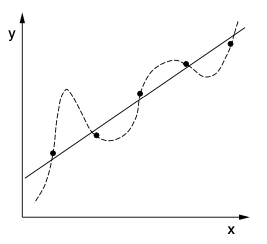
\includegraphics[width=0.5\textwidth]{Images/1.png}
    \caption{Dos posibles modelos de regresión, uno lineal y otro no, para un conjunto de datos dado. (Gráfica tomada de [1])}
    \label{fig:Sobreajuste y subajuste}
\end{figure}

La Figura ~\ref{fig:Sobreajuste y subajuste} muestra una representación gráfica de dicho conjunto de datos (indicados por los puntos redondos), 
junto con dos posibles dependencias funcionales que podrían explicar los datos. 
La línea discontinua, \(f_{\text{no lineal}}\), representa un modelo bastante complejo y ajusta perfectamente 
los datos de entrenamiento, es decir, tiene un error de entrenamiento igual a 0. Por otro lado, 
la línea recta, \(f_{\text{lineal}}\), no “explica” completamente los datos de entrenamiento, 
ya que hay algunos errores residuales, lo que genera un error de entrenamiento pequeño pero positivo 
(por ejemplo, medido mediante la función de pérdida cuadrática).\newline


¿Pero qué sucede con los riesgos verdaderos \(R(f_{\text{no lineal}})\) y \(R(f_{\text{lineal}})\)? 
El problema es que no podemos calcular estos riesgos a partir de los datos de entrenamiento. 
Además, las funciones \(f_{\text{no lineal}}\) y \(f_{\text{lineal}}\) tienen comportamientos muy diferentes. 
Por ejemplo, si la línea recta \(f_{\text{lineal}}\) fuera la verdadera función subyacente, 
entonces la función discontinua \(f_{\text{no lineal}}\) tendría un riesgo verdadero elevado, 
ya que la “distancia” entre la función verdadera y la estimada es muy grande. 
Lo mismo ocurre en sentido contrario. En ambos casos, el riesgo verdadero sería mucho mayor que el riesgo empírico.\newline


Este ejemplo resalta una decisión importante que debemos tomar: ¿preferimos ajustar los datos de entrenamiento 
con una función relativamente compleja, lo que conduce a un error de entrenamiento muy pequeño, o preferimos 
ajustarlos con una función simple a costa de un error de entrenamiento ligeramente mayor? En el ejemplo 
anterior, un físico que mida estos puntos de datos podría argumentar que no puede ser coincidencia que las mediciones 
estén casi alineadas y preferiría atribuir los residuos a errores de medición en lugar de a un modelo erróneo. Nos interesa
entonces caracterizar en qué sentido la línea recta es más simple y por qué esto debería implicar que está, de 
alguna manera, más cerca de la verdadera dependencia subyacente. Es decir, nos interesa saber cuál es el 
aumento en el error de entrenamiento que deberíamos estar dispuestos a tolerar para ajustar un modelo más simple. 
En la terminología del aprendizaje 
estádistico aplicado, decimos que el modelo complejo muestra \textit{sobreajuste} (overfitting), 
mientras que el modelo lineal simple es más proclive a sufrir de \textit{subajuste} (underfitting).\newline

De una forma u otra, esta cuestión ha ocupado durante mucho tiempo las mentes de los investigadores que estudian 
el problema del aprendizaje. En Estadística clásica, se ha estudiado como el dilema \textit{sesgo-varianza} 
(más conocido por su nombre en inglés, \textit{bias-variance tradeoff}). Si ajustamos un modelo lineal para cada conjunto de datos que encontramos, 
podríamos pensar que toda dependencia funcional es lineal. Pero no sería por la naturaleza de los procesos que
generan los datos, sino un sesgo impuesto por nosotros. Por otro lado, 
si tomamos un polinomio de grado suficientemente alto para cualquier muestra, siempre podríamos ajustar 
perfectamente los datos, pero el modelo exacto que obtendríamos estaría sujeto a grandes fluctuaciones, dependiendo 
de qué tan precisas fueran nuestras mediciones en primer lugar, dado que el grado y la forma del polinomio estarían más
bien determinados por el error propio de los procesos que por la función generadora en sí. Esto implicaría que el modelo 
posea una gran varianza, dado que cada posible función clasificadora creada podría alejarse mucho de otras posibles funciones 
cuando los datos de entrenamiento usados cambien.\newline

Observemos que el dilema sesgo-varianza está estrechamente unido a la cuestión del sub y sobreajuste de un modelo. En efecto,
cuando aplicamos un sesgo fuerte al aprendizaje, determinando un espacio funcional pequeño, restringimos la flexibilidad de las
funciones clasificadoras que son posibles y reducimos el riesgo de sobreajuste del modelo. Por ejemplo, dado un conjunto
de datos en $\mathbb{R}^2$ a partir del cual deseamos inferir el valor de otros puntos (un problema de regresión), es común
pensar en que puede existir una relación lineal entre las variables, por lo que podríamos restringir el espacio funcional
de clasificadores a uno lineal parametrizado por dos parámetros $\alpha, \beta$ que reprentan la pendiente y la ordenada
al origen de la recta $R: y(x) = \alpha x + \beta$. En este caso, el problema de aprendizaje es encontrar la recta que reduce
el error (usualmente, el error cuadrático medio) sobre los puntos de entrenamiento. En este caso, imponemos un sesgo
sobre el modelo que reduce la varianza del mismo, ya que al generar distintos conjuntos de entrenamiento sobre los cuales
entrenar el modelo, los distintos clasificadores resultantes no serían tan distintos entre sí (serían todas rectas con parametros,
esperablemente, parecidos).\newline


Dirijamos ahora nuestra atención al dilema restante, entre dos conceptos que llamamos \textit{estimación} y \textit{aproximación}, 
los cuales procedemos a describir. 

En estadística, llamamos \textit{estimador} a un valor, obtenible experimentalmente, que nos da indicios
de algún otro valor que no podemos obtener fácilmente (o al que es imposible acceder). Por ejemplo, es logísticamente impensable
medir a cada uno de los habitantes de un país, pero es posible estimar la altura promedio de estos a partir de muestras que tomamos
de su población. En este caso, la media muestral es un estimador de la media poblacional. 

Por otro lado, al modelizar un fenómeno de cualquier índole, hacemos uso de aproximaciones conceptuales para
hacer predicciones y obtener información valiosa. En el ejemplo anterior, podría suceder que la relación bidimensional que estamos
regresionando es una entre el consumo energético de un país y su PBI per cápita. Dicha relación difícilmente sea verdaderamente lineal,
pero una aproximación del estilo puede llevarnos a una conclusión general: No hay países pobres que consuman poca energía, o bien,
el desarrollo económico implica un aumento en el gasto energético. Esta conclusión es útil aunque no este construida sobre una descripción
perfecta del evento estudiado, si no sobre una aproximación.

Ahora bien, traslademos esto a lo que nos interesa estudiar aquí. En el contexto del Machine Learning, llamamos \textit{error de aproximación}
al error insalvable que surje de modelizar un fenómeno con una descripción imperfecta del mismo. Dado que no conocemos la distribución
de probabilidad conjunta de nuestras variables $X$ e $Y$, no podemos saber nunca cuál es realmente la naturaleza del proceso que las involucra,
si no solo aproximarla. Más formalmente, al definir un problema de aprendizaje fijando un espacio funcional de clasificadores, 
el error de aproximación es la diferencia que existe entre el mejor clasificador en dicho espacio -ya elegido- y el mejor clasificador posible,
$f_{\text{Bayes}}$.

Por otro lado, llamamos \textit{error de estimación} a la diferencia que existe entre el mejor clasificador, $f_{\mathcal{F}}$ de un espacio dado y el clasificador
que hemos construido a partir de ejemplos. Como estamos estudiando una teoría asintótica (esto es, que hace aseveraciones con límites, los cuales usualmente
son limites en el infinito), no esperamos encontrar siquiera a $f_{\mathcal{F}}$, si no simplemente estimarlo. Como la estimación depende de las muestras,
este error puede variar dependiendo de qué datos de entrenamiento tengamos. En el ejemplo de la altura de un país, podríamos obtener una muestra de chicos inusualmente
altos (quiza un equipo de basket, aunque no estaríamos ante una \textit{buena} muestra, dado que no sería iid) que nos brinde una estimación mentirosa. \newline

\begin{figure}[ht!]
    \centering
    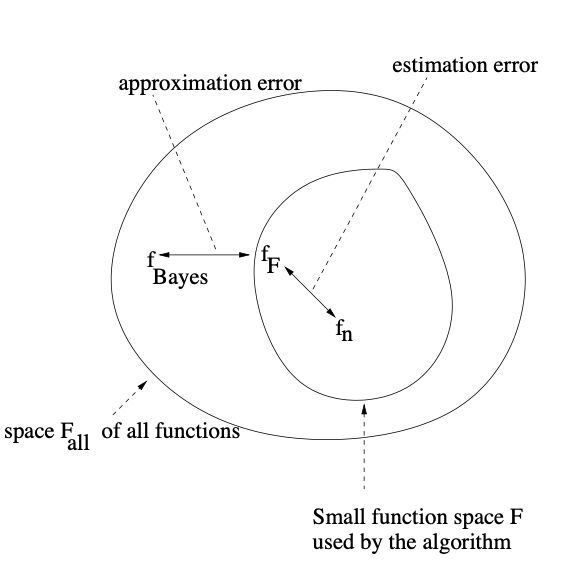
\includegraphics[width=0.5\textwidth]{Images/2.png}
    \caption{Error de estimación y de aproximación. (Gráfica tomada de [1])}
    \label{fig:error de estimación y aproximación}
\end{figure}


El ejemplo ilustrado en la Figura ~\ref{fig:Sobreajuste y subajuste}
ya señaló de manera intuitiva el problema de la complejidad del modelo: nos interesa poder entender cuando un modelo es más simple que otro,
por qué es mejor un modelo más simple.
Ya hemos mencionado anteriormente que el objetivo de la clasificación es lograr un riesgo tan bueno 
como el del clasificador de Bayes. ¿Podríamos simplemente elegir \(\mathcal{F}\) como el espacio \(\mathcal{F}_{\text{all}}\) 
de todas las funciones, definir el clasificador 
$$f_n := \arg\min_{f \in \mathcal{F}_{\text{all}}} \left(\mathcal{R}_{\text{emp}}(f)\right),$$ 
y obtener consistencia? Desafortunadamente, la respuesta es no. Luego veremos que, 
si optimizamos sobre clases de funciones \(\mathcal{F}\) demasiado grandes, y en particular si hacemos \(\mathcal{F}\) tan 
grande que contenga todos los clasificadores de Bayes para todas las distribuciones de probabilidad \(P\), 
esto conduce a la inconsistencia. Por lo tanto, si queremos aprender con éxito, necesitamos trabajar 
con una clase de funciones \(\mathcal{F}\) más pequeña. Para investigar las propiedades contrapuestas de la 
complejidad del modelo y la generalización, queremos introducir algunas nociones que serán útiles más adelante.\newline

Recordemos las definiciones \(f_n\), \(f_\mathcal{F}\) y \(f_{\text{Bayes}}\) introducidas anteriormente. Hemos visto que 
la consistencia de Bayes trata sobre la convergencia del término \(R(f_n) - R(f_{\text{Bayes}})\). 
Es importante notar que podemos descomponer esta cantidad de la siguiente manera:\newline
\[ 
\mathcal{R}(f_n) - \mathcal{R}(f_{\text{Bayes}}) = \underbrace{\mathcal{R}(f_n) - \mathcal{R}(f_\mathcal{F})}_{\text{error de generalización}} +
\underbrace{\mathcal{R}(f_\mathcal{F}) - \mathcal{R}(f_{\text{Bayes}})}_{\text{error de aproximación}} 
\]

Es decir, podemos descomponer la diferencia que determina el concepto de consistencia en dos términos que corresponden a cada uno de los errores que
hemos discutido antes. En la Figura 
\ref{fig:error de estimación y aproximación} 
tenemos una ilustración. El primer término aborda la 
incertidumbre introducida por el proceso de muestreo aleatorio. Dado un conjunto de datos 
finitos, necesitamos estimar la mejor función en \(\mathcal{F}\). Por supuesto, en este proceso cometeremos 
errores. Este error se denomina error de estimación. El segundo término no está influido por cantidades aleatorias.
Trata sobre el error que cometemos al buscar la mejor función en un espacio de funciones \(\mathcal{F}\) pequeño, 
en lugar de buscar la mejor función en el espacio \(F_{\text{all}}\) de todas las funciones posibles. 
La pregunta fundamental en este contexto es qué tan bien las funciones en \(\mathcal{F}\) pueden aproximar a las 
funciones en \(F_{\text{all}}\) y de allí proviene el nombre error de aproximación.\newline

\begin{figure}[ht!]
    \centering
    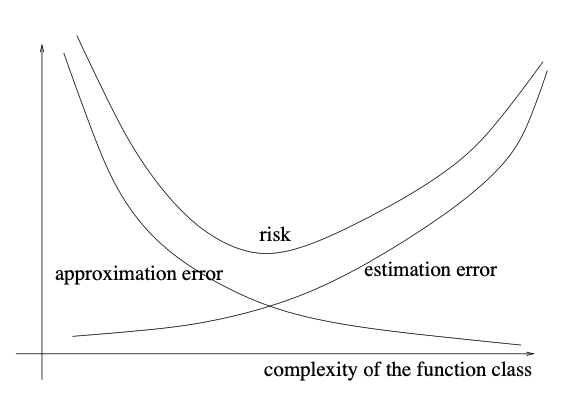
\includegraphics[width=0.5\textwidth]{Images/3.png}
    \caption{Compromiso entre error de estimación y de aproximación. Si el espacio funcional $\mathcal{F}$ que define
    el algoritmo de aprendizaje es pequeño, es decir es poco complejo, el error de estimación es bajo, pero el de aproximación
    es alto, y estamos en una situación proclive al subajuste. Si, por otro lado,  $\mathcal{F}$ es complejo, el error de estimación
    es alto y el de aproximación bajo, y tendemos al sobreajuste. El error ideal es usualmente obtenido con una complejidad moderada.
    (Gráfica tomada de [1])}
    \label{fig:Compromiso entre error de estimación y de aproximación.}
\end{figure}



Podemos señalar que el espacio \(\mathcal{F}\) es el medio para equilibrar el compromiso 
entre el error de estimación y el error de aproximación. Si elegimos un espacio \(\mathcal{F}\) muy grande, el 
término de aproximación será pequeño (el clasificador de Bayes podría incluso estar contenido en 
\(\mathcal{F}\) o ser aproximado de manera cercana por algún elemento en \(\mathcal{F}\)). Sin embargo, el error de 
estimación será bastante grande en este caso: el espacio \(\mathcal{F}\) contendrá funciones complejas que 
conducirán al \textbf{sobreajuste} (overfitting). El efecto opuesto ocurrirá si la clase de funciones 
\(\mathcal{F}\) es muy pequeña.\newline


En lo que sigue, trataremos el error de estimación y el error de aproximación por separado. Veremos 
que tienen comportamientos bastante diferentes y que se necesitan métodos distintos para controlar 
cada uno.\newline

\section{El clasificador de los $k$ vecinos más cercanos}

Hasta 1977, no se sabía si existía un clasificador universalmente consistente. 
Esta pregunta fue resuelta positivamente por Stone (1977), quien demostró, mediante una elegante prueba, 
que un clasificador particular, el denominado clasificador de los \(k\)-vecinos más cercanos 
(\textit{k-nearest neighbors classifier}, abreviado como $k$-NN), es universalmente consistente. Como el clasificador de los \(k\)-vecinos 
más cercanos es uno de los clasificadores más simples y todavía se usa ampliamente en la práctica, 
dedicaremos esta sección a ilustrar las nociones introducidas en la sección anterior, tales como 
generalización, sobreajuste, subajuste y consistencia, usando el ejemplo del clasificador \(k\)-NN.\newline

Consideremos una muestra de puntos con etiquetas \((X_1, Y_1), \dots, (X_n, Y_n)\) que 
pertenecen a un espacio métrico. De manera general, el paradigma del aprendizaje consiste en asignar salidas 
similares a entradas similares. Es decir, creemos que los puntos que están cercanos en el espacio 
de entrada tienden a tener la misma etiqueta en el espacio de salida. Nótese que si esta afirmación 
no se cumple, el aprendizaje se vuelve muy difícil o incluso imposible. Para un aprendizaje exitoso, 
debe existir alguna forma de relacionar las etiquetas de los puntos de entrenamiento con las de los 
puntos de prueba, y esto siempre implica suposiciones previas sobre las relaciones entre los puntos 
de entrada. La relación más simple es una distancia entre puntos, pero existen otras formas de medir 
la similitud, como los \textit{kernels}, que forman la base de algunos de los algoritmos 
de aprendizaje más populares (ver [5]).\newline

Supongamos entonces que existe una función de distancia en el espacio de entrada, es decir, una función 
\(d : X \times X \to \mathbb{R}\), que asigna un valor de distancia \(d(X, X')\) a cada par de puntos 
de entrenamiento \(X, X'\). Dados algunos puntos de entrenamiento, ahora queremos predecir una buena 
etiqueta para un nuevo punto \(X\) que no se halla en el conjunto de entrenamiento.
 Una idea simple es buscar el punto de entrenamiento \(X_i\) 
que tenga la distancia más pequeña a \(X\) y asignar a \(X\) la etiqueta correspondiente \(Y_i\) de 
ese punto. Para definir esto de manera más formal, denotamos por \(\text{NN}(X)\) al vecino más cercano 
de \(X\) entre todos los puntos de entrenamiento, es decir:

\[
\text{NN}(X) = \arg\min \{X' \in \{X_1, \dots, X_n\} \mid d(X, X') \leq d(X, Z)\}, 
\]
para todo \( Z \in \{X_1, \dots, X_n\} \). \newline

Luego, podemos definir el clasificador \(f_n\) basado en la muestra de \(n\) puntos como:

\[
f_n(X) = Y_i \quad \text{donde} \quad X_i = \text{NN}(X).
\]

Este clasificador se denomina clasificador de un vecino más cercano (\textit{1-nearest neighbor}, 1NN). 
Podemos generalizarlo en el clasificador de los \(k\)-vecinos más cercanos (\textit{kNN}), considerando los \(k\) puntos de 
entrenamiento más cercanos, con $k>1$ en este caso, y tomando el promedio de todas sus etiquetas. \newline


\begin{dfn}
    Dados un espacio métrico \(\mathcal{X}\) junto a una función de distancia \(d : X \times X \to \mathbb{R}\), 
    un conjunto de puntos de entrenamiento con sus etiquetas \((X_1, Y_1), \dots, (X_n, Y_n)\) y un entero \(k \geq 1\), 
    definimos los \textbf{\(k\)-vecinos más cercanos} de un punto \(X \in \mathcal{X} \) como el conjunto de los \(k\) puntos 
    de entrenamiento más cercanos a \(X\), es decir:

    \[
    \text{kNN}(X) = \{X_{i_1}, \dots, X_{i_k}\} \quad \text{donde} \quad i_1, \dots, i_k = \arg\min_{1 \leq j \leq n} d(X, X_j).
    \]
\end{dfn}

Es decir, definimos los 
\(k\)-vecinos más cercanos de \(X\), \(\text{kNN}(X)\), como el conjunto de los \(k\) puntos de 
entrenamiento más cercanos a \(X\). Luego, el clasificador \(k\)-NN se define como:

\begin{dfn}
    Con las mismas condiciones de la definición anterior,
    definimos el \textbf{clasificador de los \(k\)-vecinos más cercanos} como la función \(f_n : X \to Y\) 
    que asigna a un punto \(X\) la etiqueta que resulta de una votación mayoritaria entre las etiquetas 
    de los puntos de entrenamiento en la vecindad de \(k\)-vecinos más cercanos de \(X\):


    \[
f_n(X) = 
\begin{cases} 
+1 & \text{si } \underset{{X_i \in \text{kNN}(X)}}{\sum}Y_i > 0, \\ 
-1 & \text{en otro caso}.
\end{cases}
\]
\end{dfn}


Es decir, decidimos la etiqueta de \(X\) mediante una votación mayoritaria entre las etiquetas de los 
puntos de entrenamiento en la vecindad de \(k\)-vecinos más cercanos de \(X\). Para evitar empates, 
generalmente se elige \(k\) como un número impar.\newline


\begin{thm}
    El clasificador de un vecino más cercano (1NN) no es Bayes-consistente.
\end{thm}

\begin{proof}

Consideremos 
el intervalo real \(X = [0, 1]\) y la distribución de probabilidad \(P([0, 1])\),  que asigna etiquetas 
de manera uniforme a todos los puntos \(X \in [0, 1]\) con ruido, de modo que 
\(P(Y = 1 \mid X = x) = 0.9\) para todo \(x \in X\). Es decir, la etiqueta correcta (la que 
asigna el clasificador de Bayes) es \(+1\) para todos los puntos \(x \in X\). Ya hemos mencionado 
este ejemplo cuando introdujimos el clasificador de Bayes. En este caso, el clasificador de Bayes 
es simplemente la función que devuelve \(1\) para todos los puntos en \(X\), y su riesgo Bayesiano 
con respecto a la pérdida 0-1 será

\[
\begin{aligned}
    \mathcal{R}(f_{\text{Bayes}}) & = \mathbb{E}(\ell(X,Y,f_{\text{Bayes}}(X))) \\
    & = \mathbb{E}(1\cdot P(f_{\text{Bayes}}(X)\neq Y) + 0 \cdot P(f_{\text{Bayes}}(X) = Y))\\
    & = \mathbb{E}(P(f_{\text{Bayes}}(X)\neq Y))\\
    & = \int_{0}^{1} P(Y = 1 \mid X = x) \cdot \mathbf{1}_{\{f_{\text{Bayes}}(x) \neq 1\}} \, dx \\
    & \qquad \qquad + \int_{0}^{1} P(Y=0 \mid X=x) \cdot \mathbf{1}_{\{f_{\text{Bayes}}(x) = 1\}} \\
    & = \int_{0}^{1} (0.9 \cdot 0 + 0.1 \cdot 1) \, dx = 0.1.
\end{aligned}
\]

Ahora investiguemos el comportamiento del clasificador 1NN 
en este caso. Al tomar puntos de entrenamiento \((X_i, Y_i)_{i=1,\dots,n}\) de acuerdo con la 
distribución subyacente, estos estarán aproximadamente uniformemente distribuidos en el intervalo 
\([0, 1]\). En promedio, cada décimo punto tendrá una etiqueta de entrenamiento \(Y = -1\), y todos 
los demás tendrán etiqueta \(Y = +1\). Si ahora consideramos el comportamiento del clasificador \(f_n\), 
podemos escribir la probabilidad de que el clasificador 1NN cometa un error al etiqueta un punto como:

\[
\begin{aligned}
P(Y \neq f_n(X)) & = P(Y = 1 \mid f_n(X) = 0) + P(Y = 0 \mid f_n(X) = 1) \\
                 & = 0.1 \cdot 0.9 + 0.9 \cdot 0.1 \\
                 & = 2 \cdot 0.1 \cdot 0.9 = 0.18.
\end{aligned}
\]

Podemos ver que el riesgo \(R(f_n)\) del clasificador \(f_n\) es también $0,18$,
independientemente del tamaño de la muestra $n$. En efecto:

\[
\begin{aligned}
    \mathcal{R}(f_n) & = \mathbb{E}(\ell(X,Y,f_n(X))) \\
    & = \int_{0}^{1} 1\cdot P(Y \neq f_n(X=x)) + 0 \cdot P(Y = f_n(X=x)) \, dx \\
    & = \int_{0}^{1} P(Y \neq f_n(X=x)) \, dx \\
    & = \int_{0}^{1} 0.18 \, dx = 0.18.
\end{aligned}
\]

Por otro lado el riesgo Bayesiano es $0.1$. Por lo tanto, el clasificador $1$NN no es consistente, ya que 
\(R(f_n) \not\to R(f_{\text{Bayes}})\).\newline
\end{proof}

Consideremos por un momento el clasificador de los 100 vecinos 
más cercanos, $100-$NN. En este caso, el clasificador cometería muchos menos errores que su primo de un vecino: 
es muy poco probable tener una vecindad de 100 puntos donde la mayoría de los votos sean \(Y = -1\). 
Así, el clasificador de 100 vecinos más cercanos, aunque sigue sin ser consistente, comete un error 
menor que el clasificador 1NN.\newline

El truco para lograr consistencia está relacionado con esta observación. Esencialmente, se debe permitir 
que el tamaño \(k\) de la vecindad bajo consideración crezca con el tamaño de la muestra \(n\). Formalmente, 
se puede demostrar el siguiente teorema:\newline


\begin{thm}(\textbf{Stone, 1977})
Sea \(f_n\) el clasificador de los \(k\)-vecinos más cercanos construido 
a partir de una muestra de \(n\) puntos. Si \(n \to \infty\) y \(k \to \infty\) de modo que \(k/n \to 0\), 
entonces \(R(f_n) \to R(f_{\text{Bayes}})\) para todas las distribuciones de probabilidad \(P\). 
Es decir, la regla de clasificación \(k\)-NN es universalmente consistente con Bayes.\newline
\end{thm}

Este teorema esencialmente nos dice que si elegimos el parámetro de vecindad \(k\) de forma que crezca 
lentamente con \(n\), por ejemplo \(k \approx \log(n)\), entonces la regla de clasificación \(k\)-NN es 
universalmente Bayes-consistente.\newline

En las secciones anteriores mencionamos que la clase de funciones \(\mathcal{F}\) de la cual se elige el clasificador 
es un componente importante para la teoría del aprendizaje estadístico. En el caso del clasificador \(k\)-NN, 
esto no es tan obvio como lo será para los clasificadores que estudiaremos en secciones posteriores. 
Intuitivamente, se puede decir que, para un parámetro fijo \(k\), la clase de funciones \(\mathcal{F}_k\) es un espacio 
de funciones constantes por partes. Cuanto mayor sea \(k\), más grandes serán las vecindades de los \(k\)-vecinos 
y, por lo tanto, mayores serán los segmentos donde las funciones deben ser constantes. Esto significa que, 
para valores muy grandes de \(k\), la clase de funciones \(\mathcal{F}_k\) es relativamente pequeña (las funciones no 
pueden oscilar mucho). En el caso extremo de \(k = n\), la vecindad de los \(k\)-vecinos simplemente incluye 
todos los puntos de entrenamiento, por lo que el clasificador \(k\)-NN no puede cambiar su signo en absoluto; 
debe ser constante en todo el espacio de entrada \(\mathcal{X}\). En este caso, la clase de funciones \(\mathcal{F}_k\) contiene solo 
dos elementos: la función que es constantemente \(+1\) y la función que es constantemente \(-1\).\newline

Por otro lado, si \(k\) es pequeño, entonces \(\mathcal{F}_k\) se vuelve bastante grande (las funciones pueden cambiar sus 
etiquetas con mucha frecuencia y de manera abrupta). En los términos explicados en las secciones anteriores, 
podemos decir que si elegimos \(k\) demasiado pequeño, entonces la clase de funciones sobreajusta; 
por ejemplo, esto ocurre en el caso extremo del clasificador 1NN. Por el contrario, si \(k\) es demasiado grande, 
la clase de funciones subajusta, ya que simplemente no contiene funciones capaces de modelar los 
datos de entrenamiento.

\section{Minimización del riesgo empírico}

En la sección anterior encontramos nuestro primer clasificador simple: el clasificador \(k\)-NN. En esta sección, 
queremos abordar una forma más poderosa de clasificar datos, el llamado principio de \textbf{minimización 
del riesgo empírico}. Recordemos la suposición de que los datos son generados de manera \textit{iid} 
(independientes e idénticamente distribuidos) a partir de una distribución subyacente desconocida \(P(X, Y)\). 
Como ya hemos visto, el problema de aprendizaje consiste en minimizar el riesgo (o pérdida esperada sobre 
los datos de prueba):

\[
\mathcal{R}(f) = \mathbb{E}(\ell(X, Y, f(X))),
\]

donde \(f\) es una función que mapea el espacio de entrada \(\mathcal{X}\) al espacio de etiquetas \(\mathcal{Y}\), y \(\ell\) 
es la función de pérdida.\newline

La dificultad de esta tarea radica en el hecho de que estamos intentando minimizar una cantidad que no 
podemos evaluar directamente: dado que no conocemos la distribución de probabilidad subyacente \(P\), 
no podemos calcular el riesgo \(\mathcal{R}(f)\). Sin embargo, lo que sí conocemos son los datos de entrenamiento, 
muestreados a partir de \(P\). Por lo tanto, podemos intentar inferir una función \(f\) a partir de la muestra 
de entrenamiento cuyo riesgo esté cercano al mejor riesgo posible. Para ello, necesitamos lo que se llama 
un \textit{principio de inducción}.\newline

Quizás la forma más directa de proceder sea aproximar el riesgo verdadero mediante el \textbf{riesgo empírico} 
calculado sobre los datos de entrenamiento. En lugar de buscar una función que minimice el riesgo verdadero 
\(\mathcal{R}(f)\), intentamos encontrar aquella que minimice el riesgo empírico:

\[
\mathcal{R}_{\text{emp}}(f) = \frac{1}{n} \sum_{i=1}^{n} \ell(X_i, Y_i, f(X_i)).
\]

Es decir, dados algunos datos de entrenamiento \((X_1, Y_1), \dots, (X_n, Y_n)\), un espacio de funciones 
\(F\) con el cual trabajar, y una función de pérdida \(\ell\), definimos el clasificador \(f_n\) como la función:

\[
f_n := \arg\min_{f \in \mathcal{F}} \mathcal{R}_{\text{emp}}(f).
\]

Este enfoque se denomina \textbf{principio de inducción de minimización del riesgo empírico}, abreviado como 
ERM (\textit{Empirical Risk Minimization}). La motivación para este principio está dada por la ley de los 
grandes números, como explicaremos a continuación.

\subsection{Aplicando la ley de los grandes números}

Recordemos que, en su forma más simple, la ley de los grandes números
establece que, bajo condiciones suaves, la media de variables aleatorias \(\xi_i\) que han sido extraídas 
de manera \textit{iid} (independiente e idénticamente distribuida) a partir de una distribución de probabilidad 
\(P\), converge a la media de la distribución subyacente cuando el tamaño de la muestra tiende a infinito:

\[
\frac{1}{n} \sum_{i=1}^n \xi_i \to \mathbb{E}(\xi) \quad \text{cuando } n \to \infty.
\]

Aquí, la notación supone que la secuencia \(\xi_1, \xi_2, \dots\) ha sido muestreada de manera \textit{iid} 
a partir de \(P\) y que \(\xi\) también está distribuida según \(P\). Este teorema puede aplicarse al caso del 
riesgo empírico y el riesgo verdadero. Para ver esto, notemos que el riesgo empírico se define como la media de 
la pérdida \(\ell(X_i, Y_i, f(X_i))\) en puntos de muestra individuales, y el riesgo verdadero es la media de 
esta pérdida sobre toda la distribución. Es decir, a partir de la ley de los grandes números, podemos concluir 
que, para una función fija \(f\), el riesgo empírico converge al riesgo verdadero a medida que el tamaño de la 
muestra tiende a infinito:

\[
\mathcal{R}_{\text{emp}}(f) = \frac{1}{n} \sum_{i=1}^n \ell(X_i, Y_i, f(X_i)) \to \mathbb{E}(\ell(X, Y, f(X))) \quad 
\text{cuando } n \to \infty.
\]

Aquí, la función de pérdida \(\ell(X, Y, f(X))\) desempeña el papel de la variable aleatoria \(\xi\). Para una 
muestra finita dada, esto significa que podemos aproximar el riesgo verdadero (el que nos interesa) de manera 
bastante precisa mediante el riesgo empírico (el que podemos calcular sobre la muestra).\newline

Una desigualdad famosa, atribuida a Chernoff (1952) y luego generalizada por Hoeffding (1963), caracteriza qué 
tan bien la media empírica aproxima el valor esperado. Específicamente, si las variables aleatorias \(\xi_i\) 
toman valores solo en el intervalo \([0, 1]\), entonces:

\begin{equation}\label{eq:Chernoff-Hoeffding}
P\left( \left| \frac{1}{n} \sum_{i=1}^n \xi_i - \mathbb{E}(\xi) \right| \geq \varepsilon \right) \leq 
2 \exp(-2n\varepsilon^2). 
\end{equation}\newline

Este teorema establece que la probabilidad de que la media de la muestra se desvíe más de \(\varepsilon\) del 
valor esperado de la distribución está acotada por una cantidad muy pequeña, específicamente \(2 \exp(-2n\varepsilon^2)\). 
Nótese que, cuanto mayor sea \(n\), más pequeña será esta cantidad; es decir, la probabilidad de desviaciones 
grandes disminuye rápidamente con \(n\). Una vez más, podemos aplicar este teorema al contexto del riesgo empírico 
y verdadero. Esto conduce a una cota que establece qué tan probable es que el riesgo empírico esté cerca del 
riesgo verdadero para una función dada \(f\):

\begin{equation}
P(|\mathcal{R}_{\text{emp}}(f) - \mathcal{R}(f)| \geq \varepsilon) \leq 2 \exp(-2n\varepsilon^2).  \label{eq:Chernoff}
\end{equation}

Para cualquier función fija (y un \(n\) suficientemente grande), es muy probable que el error de entrenamiento 
proporcione una buena estimación del error de prueba.\newline

Existen algunos hechos importantes relacionados con la cota de Chernoff (\ref{eq:Chernoff}). Primero, una propiedad crucial 
de la cota de Chernoff es que es de naturaleza probabilística. Establece que la probabilidad de una gran desviación 
entre el error de prueba y el error de entrenamiento de \(f\) es pequeña; cuanto mayor sea el tamaño de la muestra 
\(n\), menor será esta probabilidad. Por lo tanto, no descarta la presencia de casos en los que la desviación sea 
grande; simplemente dice que, para una función fija \(f\), esto es muy poco probable. La razón de esto radica en la 
generación aleatoria de los puntos de entrenamiento. Podría ocurrir que, en algunos casos desafortunados, nuestros 
datos de entrenamiento sean tan engañosos que sea imposible construir un buen clasificador a partir de ellos. Sin 
embargo, a medida que el tamaño de la muestra aumenta, tales casos desafortunados se vuelven muy raros. En este 
sentido, cualquier garantía de consistencia solo puede ser de caracter probabilístico: el riesgo empírico está cerca del riesgo 
verdadero, con alta probabilidad.\newline

A primera vista, parece que la cota de Chernoff (\ref{eq:Chernoff}) es suficiente para probar la consistencia de la minimización 
del riesgo empírico. Sin embargo, hay una advertencia importante: la cota de Chernoff solo se cumple para una función 
fija \(f\) que no depende de los datos de entrenamiento. Sin embargo, el clasificador \(f_n\), por supuesto, depende 
de los datos de entrenamiento (usamos los datos de entrenamiento para seleccionar \(f_n\)). Aunque esto pueda parecer 
una diferencia matemática sutil, aquí es donde la minimización del riesgo empírico puede fallar por completo. A 
continuación, discutiremos este problema en detalle y veremos cómo adaptar la ley fuerte de los grandes números para 
poder tratar funciones que dependen de los datos.\newline

\subsection{Inconsistencia en la minimización del riesgo empírico} \label{Inconsistencia en la minimización del riesgo empírico}

Supongamos que nuestro espacio de datos subyacente es \(X = [0,1]\). Elegimos la distribución uniforme sobre 
\(\mathcal{X}\) como la distribución de probabilidad y definimos la etiqueta \(Y\) para un punto de entrada \(X\) de 
manera determinista como sigue:

\[
Y = 
\begin{cases} 
-1 & \text{si } X < 0.5, \\ 
1 & \text{si } X \geq 0.5.
\end{cases}
\]

Ahora supongamos que se nos da un conjunto de puntos de entrenamiento \((X_i, Y_i)_{i=1,\dots,n}\) y 
consideremos el siguiente clasificador:

\[
f_n(X) = 
\begin{cases} 
Y_i & \text{si } X = X_i \text{ para algún } i = 1, \dots, n, \\ 
1 & \text{en otro caso.}
\end{cases}
\]

Este clasificador \(f_n\) clasifica perfectamente todos los puntos de entrenamiento. Es decir, tiene un 
riesgo empírico \(\mathcal{R}_{\text{emp}}(f_n) = 0\). En consecuencia, dado que el riesgo empírico no puede ser 
negativo, \(f_n\) es un minimizador del riesgo empírico. Sin embargo, \(f_n\) claramente no ha aprendido 
nada; el clasificador simplemente memoriza las etiquetas de entrenamiento y, en otros casos, predice 
simplemente la etiqueta \(1\).\newline

Formalmente, esto significa que el clasificador \(f_n\) no será consistente. Para ver esto, supongamos que 
se nos da un punto de prueba \((X, Y)\) extraído de la distribución subyacente. Usualmente, este punto de 
prueba no será idéntico a ninguno de los puntos de entrenamiento, y en este caso el clasificador simplemente 
predice la etiqueta \(1\). Si \(X\) resulta ser mayor que \(0.5\), esta es la etiqueta correcta, pero si 
\(X < 0.5\), es la etiqueta incorrecta. Por lo tanto, el clasificador \(f_n\) cometerá errores en la mitad 
de todos los puntos de prueba, lo que implica que su error de prueba es \(R(f_n) = 1/2\). Este es el mismo 
error que se obtendría con una predicción aleatoria. De hecho, este es un buen ejemplo de 
\textbf{sobreajuste}: el clasificador \(f_n\) se ajusta perfectamente a los datos de entrenamiento, pero no 
aprende nada sobre los nuevos datos de prueba.\newline

Es fácil ver que el clasificador \(f_n\) es inconsistente. Nótese que, como las etiquetas son una función 
determinista de los puntos de entrada, el clasificador de Bayes tiene un riesgo igual a \(0\). Así, tenemos:

\[
\frac{1}{2} = R(f_n) \not\to R(f_{\text{Bayes}}) = 0.
\]

Hemos construido un ejemplo donde la minimización del riesgo empírico falla de manera estrepitosa. ¿Existe 
alguna manera de rescatar el principio de ERM? Afortunadamente, la respuesta es sí. El objeto principal al 
que debemos prestar atención es la clase de funciones \(\mathcal{F}\) de la cual extraemos nuestro clasificador. Si 
permitimos que nuestra clase de funciones contenga funciones que simplemente memorizan los datos de 
entrenamiento, entonces el principio de ERM no puede funcionar. En particular, si elegimos el minimizador 
del riesgo empírico del espacio \(F_{\text{all}}\) de todas las funciones entre \(\mathcal{X}\) e \(\mathcal{Y}\), entonces los 
valores de \(f_n\) en los puntos de entrenamiento \(X_1, \dots, X_n\) no necesariamente contienen ninguna 
información sobre los valores en otros puntos. Por lo tanto, a menos que impongamos restricciones en el 
espacio de funciones del cual elegimos nuestra estimación \(f\), no podemos esperar aprender nada.\newline


\subsection{Convergencia uniforme}

Resulta que las condiciones necesarias para que la minimización del riesgo empírico sea consistente 
implican restringir el conjunto de funciones admisibles. La idea principal de la teoría de Vapnik-Chervonenkis 
(VC), en la cual profundizaremos en el segundo capítulo, es que la consistencia de la minimización del riesgo empírico está determinada por el comportamiento 
en el peor caso sobre todas las funciones \(f \in \mathcal{F}\) que la máquina de aprendizaje podría elegir. Veremos que, 
en lugar de la ley estándar de los grandes números introducida anteriormente, este caso extremo corresponde 
a una versión de la ley de los grandes números que es uniforme sobre todas las funciones en \(\mathcal{F}\).

\begin{figure}[ht!]
    \centering
    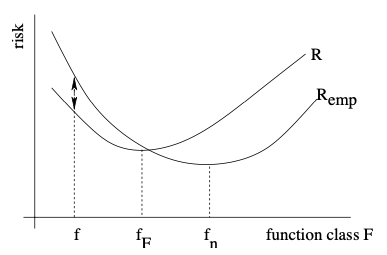
\includegraphics[width=0.8\textwidth]{Images/4.png}
    
    \caption{Representación simplificada de la convergencia del riesgo empírico al riesgo verdadero. El eje \(x\) 
    representa una dimensión de la clase de funciones \(F\), mientras que el eje \(y\) denota el riesgo. Para cada 
    función fija \(f\), la ley de los grandes números nos dice que, a medida que el tamaño de la muestra tiende a 
    infinito, el riesgo empírico \(\mathcal{R}_{\text{emp}}(f)\) converge al riesgo verdadero \(\mathcal{R}(f)\) (indicado por la flecha). 
    Sin embargo, esto no implica que, en el límite de tamaños de muestra infinitos, el minimizador del riesgo 
    empírico, \(f_n\), lleve a un valor del riesgo tan bueno como el del mejor \(f_F\) en la clase de funciones. 
    Para que esto sea cierto, requerimos la convergencia uniforme de \(\mathcal{R}_{\text{emp}}(f)\) a \(\mathcal{R}(f)\) sobre todas 
    las funciones en \(F\). (Grafico adaptado de [5].}
    \label{riesgo vs riesgo empirico}
    \end{figure}
    
La Figura \ref{riesgo vs riesgo empirico} nos muestra una representación simplificada de la ley uniforme de los grandes números y la cuestión 
de la consistencia. Tanto el riesgo empírico como el riesgo verdadero se grafican como funciones de \(f\). 
Para simplificar, hemos resumido todas las funciones posibles \(f\) en un solo eje del gráfico. La minimización 
del riesgo empírico consiste en elegir la función \(f\) que minimiza \(\mathcal{R}_{\text{emp}}\). Es consistente si el 
mínimo de \(\mathcal{R}_{\text{emp}}\) converge al de \(R\) a medida que el tamaño de la muestra aumenta. Una forma de 
garantizar la convergencia del mínimo para todas las funciones en \(\mathcal{F}\) es la convergencia uniforme sobre 
\(\mathcal{F}\): requerimos que para todas las funciones \(f \in \mathcal{F}\), la diferencia entre \(\mathcal{R}(f)\) y \(\mathcal{R}_{\text{emp}}(f)\) 
se vuelva pequeña simultáneamente. Es decir, requerimos que exista un valor grande de \(n\) tal que, para un 
tamaño de muestra al menos \(n\):

\[
\sup_{f \in \mathcal{F}} |\mathcal{R}(f) - \mathcal{R}_{\text{emp}}(f)| \leq \varepsilon.
\]

Luego

\[
|\mathcal{R}(f) - \mathcal{R}_{\text{emp}}(f)| \leq \sup_{f \in \mathcal{F}} |\mathcal{R}(f) - \mathcal{R}_{\text{emp}}(f)|.
\]

En particular, esto también se cumple para una función \(f_n\) que se haya elegido en base a una muestra finita 
de puntos de entrenamiento

\begin{equation}
P(|R(f_n) - \mathcal{R}_{\text{emp}}(f_n)| \geq \varepsilon) \leq P\left(\sup_{f \in \mathcal{F}} |\mathcal{R}(f) - \mathcal{R}_{\text{emp}}(f)| \geq \varepsilon\right). \label{eq:cota_uniforme}
\end{equation}

La cantidad en el lado derecho de la ecuación (\ref{eq:cota_uniforme}) es ahora el objeto de la ley uniforme de los grandes números. 
Decimos que la ley de los grandes números se cumple de manera uniforme sobre una clase de funciones \(\mathcal{F}\) si, 
para todo \(\varepsilon > 0\),

\[
P\left(\sup_{f \in \mathcal{F}} |\mathcal{R}(f) - \mathcal{R}_{\text{emp}}(f)| \geq \varepsilon \right) \to 0 \quad \text{cuando } n \to \infty.
\]

Ahora podemos usar la ecuación (\ref{eq:cota_uniforme}) para mostrar que, si la ley uniforme de los grandes números se cumple para 
alguna clase de funciones \(\mathcal{F}\), entonces la minimización del riesgo empírico es consistente con respecto a \(\mathcal{F}\). 
Para verlo, consideremos:

\[
|R(f_n) - R(f_\mathcal{F})| = R(f_n) - R(f_\mathcal{F})
\]

Puesto que  \(R(f_n) - R(f_\mathcal{F}) \geq 0\), por definición de \(f_\mathcal{F}\). Sumando y restando cantidades idénticas,
esta expresión se puede reescribir como:
\[
R(f_n) - \mathcal{R}_{\text{emp}}(f_n) + \mathcal{R}_{\text{emp}}(f_n) - \mathcal{R}_{\text{emp}}(f_\mathcal{F}) + \mathcal{R}_{\text{emp}}(f_F) - R(f_\mathcal{F})
\]
\[
    \leq R(f_n) - \mathcal{R}_{\text{emp}}(f_n) + \mathcal{R}_{\text{emp}}(f_\mathcal{F}) - R(f_\mathcal{F})
\] 
\[
    \leq 2 \sup_{f \in \mathcal{F}} |\mathcal{R}(f) - \mathcal{R}_{\text{emp}}(f)|.
\]
Dado que \(\mathcal{R}_{\text{emp}}(f_n) - \mathcal{R}_{\text{emp}}(f_\mathcal{F}) \leq 0\) por definición de \(f_n\), y luego acotando
al tomar el supremo de todas las funciones en el espacio $\mathcal{F}$.\\

De esto podemos concluir:

\[
P\left(|R(f_n) - R(f_\mathcal{F})| \geq \varepsilon \right) \leq P\left(\sup_{f \in \mathcal{F}} |\mathcal{R}(f) - \mathcal{R}_{\text{emp}}(f)| \geq \varepsilon/2\right).
\]

Bajo la ley uniforme de los grandes números, el lado derecho tiende a \(0\), lo que lleva a la consistencia de 
la minimización del riesgo empírico con respecto a la clase de funciones subyacente \(\mathcal{F}\). En otras palabras, 
la convergencia uniforme sobre \(\mathcal{F}\) es una condición suficiente para la consistencia de la minimización del 
riesgo empírico sobre \(\mathcal{F}\).\newline

Parte de la elegancia de la teoría VC radica en que el recíproco también es cierto. Es decir, 
la convergencia uniforme no solo es una condición suficiente, sino también una condición necesaria para la 
consistencia de la minimización del riesgo empírico con respecto a \(\mathcal{F}\). Esto se formaliza en el siguiente 
teorema:\newline

\begin{thm}[Vapnik y Chervonenkis, 1971]
La convergencia uniforme
    
    \[
        P\left(\sup_{f \in \mathcal{F}} |\mathcal{R}(f) - \mathcal{R}_{\text{emp}}(f)| > \varepsilon \right) \to 0 \quad \text{cuando } n \to \infty, 
        \]
        
        para todo \(\varepsilon > 0\), es una condición necesaria y suficiente para la consistencia de la minimización del 
        riesgo empírico con respecto a \(\mathcal{F}\).\newline
\end{thm}
        
En la sección \ref{Inconsistencia en la minimización del riesgo empírico} dimos un ejemplo donde consideramos el conjunto de todas las funciones posibles y mostramos 
que el aprendizaje era imposible. Ahora, la dependencia del aprendizaje en el conjunto de funciones subyacente 
ha regresado bajo una forma diferente: la condición de convergencia uniforme depende críticamente del conjunto 
de funciones para el cual debe cumplirse.\newline

Intuitivamente, parece claro que cuanto mayor sea el espacio de funciones \(\mathcal{F}\), mayor será:

\[
\sup_{f \in \mathcal{F}} |\mathcal{R}(f) - \mathcal{R}_{\text{emp}}(f)|.
\]

Por lo tanto, cuanto mayor sea \(\mathcal{F}\), mayor será la medida de probabilidad:

\[
P\left(\sup_{f \in \mathcal{F}} |\mathcal{R}(f) - \mathcal{R}_{\text{emp}}(f)| > \varepsilon \right).
\]

En consecuencia, cuanto mayor sea \(\mathcal{F}\), más difícil será satisfacer la ley uniforme de los grandes números. 
Esto implica que para espacios de funciones más grandes, la consistencia es más difícil de lograr en comparación 
con espacios de funciones más pequeños.\newline


Esta caracterización abstracta de la consistencia como una propiedad de convergencia uniforme es teóricamente 
fascinante, pero no siempre es útil en la práctica. La razón es que parece complicado determinar si la ley uniforme 
de los grandes números se cumple para una clase de funciones \(\mathcal{F}\) particular. Por esta razón, se han desarrollado 
herramientas como la dimensión VC para analizar y limitar la capacidad de las clases de funciones, lo cual discutiremos 
en las siguientes secciones.\newline

\section{Cotas de generalización y medidas de capacidad}

Para hacer afirmaciones sobre lo que ocurre después de observar solo un número finito de puntos de datos 
—que en la práctica será siempre el caso—, necesitamos examinar más de cerca la 
convergencia uniforme del riesgo empírico al verdadero.\newline

Resultará que esto nos proporcionará cotas sobre el riesgo y también nos dará información sobre 
qué propiedades de las clases de funciones determinan si la convergencia uniforme puede tener lugar. Detengámonos
en la probabilidad del Teorema anterior:

\begin{equation}
P\left(\sup_{f \in \mathcal{F}} |\mathcal{R}(f) - \mathcal{R}_{\text{emp}}(f)| > \varepsilon \right). \label{eq:med_unif_riesgo_riesgo_emp}
\end{equation}

Consideremos entonces un espacio de funciones finito, como el que nos encontramos en la práctica. Sea
\(\mathcal{F}_{emp} = \{f_1, f_2, \dots, f_m\}\) un conjunto de \(m\) funciones. Cada una de las funciones 
\(f_i \in \mathcal{F}_{emp}\) satisface la ley estándar de los grandes números en la forma de la cota de Chernoff:

\[
P\left(|R(f_i) - \mathcal{R}_{\text{emp}}(f_i)| \geq \varepsilon \right) \leq 2 \exp(-2n\varepsilon^2).
\]

Ahora queremos transformar estas afirmaciones sobre funciones individuales \(f_i\) en una ley uniforme de los 
grandes números. Dada la subatividad de la probabilidad, tenemos:

\[
P\left(\sup_{f \in \mathcal{F}} |\mathcal{R}(f) - \mathcal{R}_{\text{emp}}(f)| \geq \varepsilon \right) \leq \sum_{i=1}^m P\left(|R(f_i) - \mathcal{R}_{\text{emp}}(f_i)| \geq \varepsilon \right).
\]

Y aplicando la cota de Chernoff a cada término en la suma, obtenemos:

\begin{equation}
P\left(\sup_{f \in \mathcal{F}} |\mathcal{R}(f) - \mathcal{R}_{\text{emp}}(f)| \geq \varepsilon \right) \leq 2m \exp(-2n\varepsilon^2). \label{eq: chernoff acotada por m}
\end{equation}

Si el espacio de funciones \(\mathcal{F}_{emp}\) es fijo, \(m\) puede considerarse una 
constante, y el término \(2m \exp(-2n\varepsilon^2)\) converge a \(0\) cuando \(n \to \infty\). Por lo tanto,
la minimización del riesgo empírico sobre un conjunto finito de funciones es consistente con respecto 
a \(\mathcal{F}_{emp}\). \\

En la práctica, nuestros espacios de funciones estarán definidos por los paramétros que nos permitimos 
seleccionar para cada posible clasificador, como la ordenada al origen y la pendiente en el caso de la regresión lineal y serán usualmente
, como en ese ejemplo,
espacios infinitos. Luego veremos que podemos llegar a una desigualdad similar a esta última, reemplazando $m$ por un valor que depende
de cada tipo de espacio funcional y que, de ser finito, será necesariamente polinómico, lo que nos permitirá obtener cotas de generalización.
Llamaremos a dicha cantidad, la \textit{dimensión VC}.\newline

\subsection{Simetrización}

La \textit{simetrización} es un paso técnico importante para usar medidas de capacidad en espacios infinitos de 
funciones. Su propósito principal es reemplazar el evento 

\[
\sup_{f \in \mathcal{F}} |\mathcal{R}(f) - \mathcal{R}_{\text{emp}}(f)|
\]

por un evento alternativo que pueda calcularse únicamente en una muestra dada. Supongamos que tenemos una muestra 
\((X_i, Y_i)_{i=1,\dots,n}\). Ahora introducimos una nueva muestra llamada \textit{muestra fantasma}. 
Esta es simplemente otra muestra \((X'_i, Y'_i)_{i=1,\dots,n}\), que también se extrae de manera 
\textit{iid} de la misma distribución subyacente y que es independiente de la primera muestra. No necesitamos generar 
esta muestra en la práctica; es solo una herramienta matemática para realizar el análisis. \newline

Dfinimos el riesgo empírico con respecto a esta muestra como \(\mathcal{R}'_{\text{emp}}(f)\). 
Con la ayuda de esta muestra fantasma, podemos demostrar el siguiente resultado:\newline

\begin{lem}[de simetrización] \label{lema de simetrizacion}

Sea $m\varepsilon^2 \geq 2$. Sea $\mathcal{F}$ el espacio de funciones definido por un algoritmo de aprendizaje. Sean
$(X_i,Y_i)_{i=1,\dots, n}$, $(X_i',Y_i')_{i=1,\dots, n}$ muestras aleatorias iid. Dada $f \in\mathcal{F}$,
sean $\mathcal{R}(f)$ su riesgo, $\mathcal{R}_{emp}(f)$ su riesgo empírico sobre la primera muestra y 
$\mathcal{R}'_{emp}(f)$ el riesgo sobre la segunda. Entonces, para cualquier $\varepsilon > 0$

\[
P\left(\sup_{f \in \mathcal{F}} |\mathcal{R}(f) - \mathcal{R}_{\text{emp}}(f)| > 
\varepsilon \right) \leq 2P\left(\sup_{f \in \mathcal{F}} |\mathcal{R}_{\text{emp}}(f) - \mathcal{R}'_{\text{emp}}(f)| > \frac{\varepsilon}{2}\right).
\]\newline
\end{lem}

Esta desigualdad, nos permite acotar el comportamiento 
de la diferencia \(\mathcal{R}(f) - \mathcal{R}_{\text{emp}}(f)\) mediante la diferencia entre riesgos empíricos \(\mathcal{R}_{\text{emp}}(f)\) y 
\(\mathcal{R}'_{\text{emp}}(f)\) calculados sobre las muestras original y fantasma, respectivamente. Esto nos permite trabajar 
con eventos que depende únicamente de las muestras observadas.\newline

Notemos que, incluso si \(\mathcal{F}\) contiene un número infinito de funciones, 
las diferentes formas en que estas pueden clasificar un conjunto de entrenamiento de \(n\) puntos de muestra 
es finita. En efecto, para cualquier punto de entrenamiento dado en la muestra, una función puede tomar solo los valores 
\(-1\) o \(+1\). En una muestra de \(n\) puntos \(\{X_1, \dots, X_n\}\), una función puede actuar de, como 
máximo, \(2^n\) formas diferentes: puede asignar a cada \(Y_i\) el valor \(-1\) o \(+1\). Esto tiene una 
consecuencia muy importante. Incluso si una clase de funciones \(\mathcal{F}\) contiene infinitas funciones, hay como 
mucho \(2^n\) formas diferentes en que esas funciones pueden clasificar los puntos de una muestra finita de 
\(n\) puntos. Tomando

\[
\sup_{f \in \mathcal{F}} |R_{\text{emp}}(f) - R'_{\text{emp}}(f)|,
\]
entonces el supremo efectivamente solo recorre una clase de funciones finita. Para entender esto, notemos que 
dos funciones \(f, g \in \mathcal{F}\) que toman los mismos valores en la muestra dada tienen el mismo riesgo empírico, 
es decir, \(R_{\text{emp}}(f) = R_{\text{emp}}(g)\). La afirmación análoga se cumple para la muestra fantasma 
y el riesgo empírico asociado \(R'_{\text{emp}}\). \newline

\begin{figure}[ht]
    \centering
    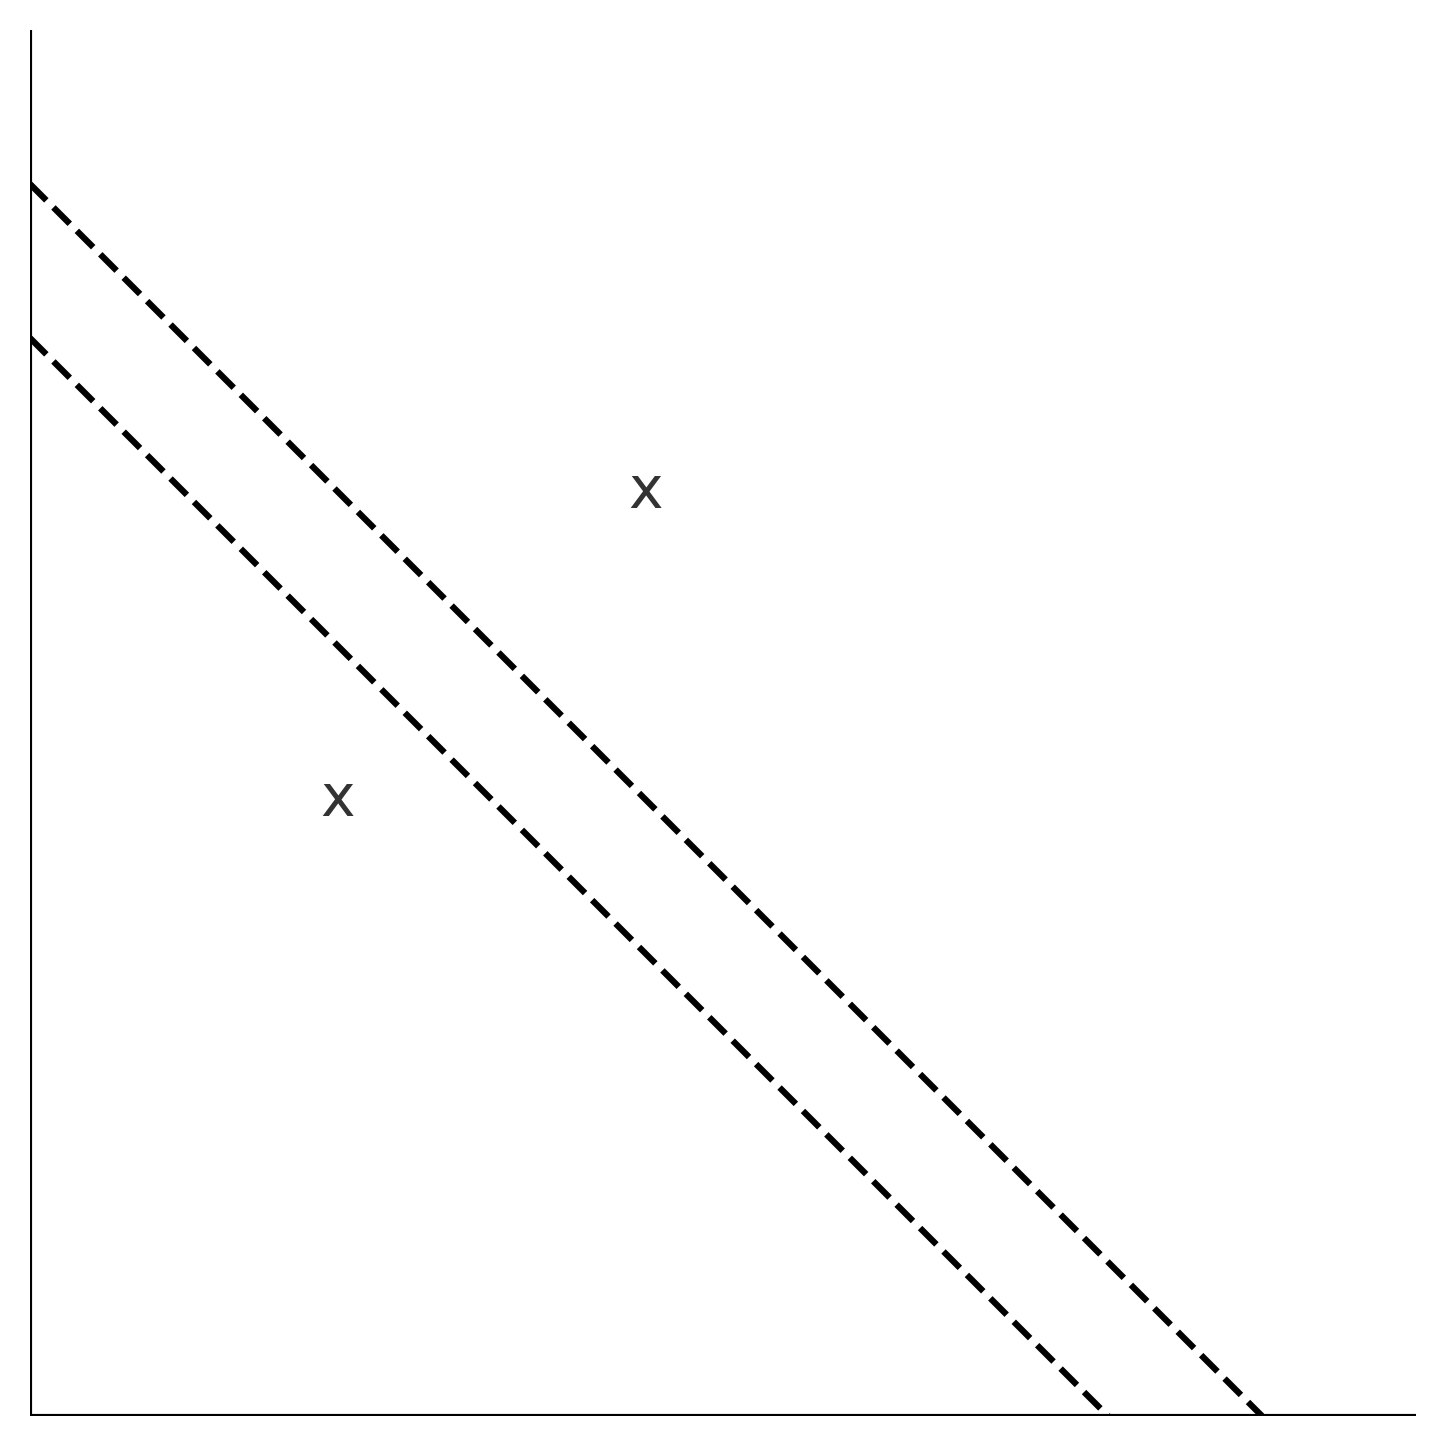
\includegraphics[width=0.8\textwidth]{Images/8.png}
    
    \caption{Dos puntos en $\mathbb{R}^2$ son clasificados de igual manera por dos clasificadores distintos.}
    \label{clasificacion identica con distintos clasificadores}
\end{figure}

Por lo tanto, todas las funciones \(f, g\) que coinciden tanto en la muestra original como en la muestra fantasma 
producirán el mismo término \(|R_{\text{emp}}(f) - R'_{\text{emp}}(f)|\). Así, las únicas funciones que 
necesitamos considerar para calcular el supremo son las \(2^{n}\) funciones que podemos obtener en la muestra 
original y la muestra fantasma juntas. Por lo tanto, podemos reemplazar el supremo sobre \(f \in \mathcal{F}\) por el 
supremo sobre una clase finita de funciones con como máximo \(2^{n}\) funciones.\newline


\subsection{El coeficiente de fragmentación}

Con la intención de analizar más a fondo la capacidad de una clase de funciones 
\(\mathcal{F}\), intentaremos acotar la medida (\ref{eq:med_unif_riesgo_riesgo_emp}).
Para esto, introducimos el concepto de coeficiente de fragmentación.  Este coeficiente mide la 
cantidad de formas en que las funciones de \(\mathcal{F}\) pueden separar los puntos de cualquier muestra
tomada sobre $X$\newline

\begin{dfn}
    Sean \(\mathcal{F}\) una clase de funciones y \(Z_n := \{(X_1, Y_1), \dots, (X_n, Y_n)\}\) un conjunto de \(n\) puntos
    etiquetados. Definimos la relación $\sim$ sobre \(\mathcal{F}\):
        \[
        f_1 \sim f_2 \qquad \text{si} \qquad f_1(X_i) = f_2(X_i) \quad \forall i = 1, \dots, n.
        \]
\end{dfn}
\begin{obs}
    La relación \(\sim\) es una relación de equivalencia sobre \(\mathcal{F}\). Luego, para una muestra fija,
    define una partición sobre $X$.
\end{obs}
\begin{dfn}
    Definimos el \textbf{conjunto de fragmentación} \(\mathcal{F}_{Z_n}\) a cualquier conjunto de representantes de \(\mathcal{F}\)
    bajo la relación de equivalencia \(\sim\) .
\end{dfn}
\begin{dfn}
    Dado un espacio muestral $X$ y \(Z_n := \{(X_1, Y_1), \dots, (X_n, Y_n)\}\) una muestra de tamaño \(n\). Definimos el 
    \textbf{coeficiente de fragmentación} del espacio funcional $\mathcal{F}$ como:
    
    \[
    \mathcal{N}(\mathcal{F}, n) = \max_{Z_n} \{|\mathcal{F}_{Z_n}|\} = \max_{\{X_1, \dots, X_n\}}\{|\mathcal{F}_{\{X_1, \dots, X_n\}}| \mid X_1, \dots, X_n \in X\}. 
    \]
\end{dfn}

El coeficiente $\mathcal{N}(\mathcal{F}, n)$ tiene una interpretación sencilla: mide cuántos conjuntos de etiquetas 
\( \{Y_1, \dots, Y_n\} \) pueden ser generados por las funciones de \(\mathcal{F}\), considerando todas las posibles
muestras de tamaño \(n\). Es decir, es el número de formas en las que \(\mathcal{F}\) puede separar en dos clases al 
espacio de entrada $X$.\newline

En el caso de clasificación binaria, como el que estamos tratando, el mayor cardinal posible para un conjunto de fragmentación
coincide con el cardinal del conjunto de partes de un conjunto de tamaño $n$ (basta considerar cada subconjunto posible del mismo
como aquel donde el clasificador etiqueta con $+1$ todos los valores en el subconjunto y con $-1$ los valores fuera de él). Entonces,
si \(\mathcal{N}(\mathcal{F}, n) = 2^n\), existe al menos una muestra de tamaño \(n\) que puede ser separada 
de todas las formas posibles por funciones en \(\mathcal{F}\). En este caso, decimos que la clase de funciones 
\(\mathcal{F}\) \textit{fragmenta} al conjunto de \(n\) puntos.\newline

En la definición, tomamos el máximo puesto que ciertas muestras pueden no ser fragmentables de la misma manera que otras por \(\mathcal{F}\). 
Consideremos el espacio $\mathbb{R}^2$ y sea $\mathcal{F}=\{f: f(x)= \alpha x + \beta; \; \alpha, \beta\in\mathbb{R}\}$, el espacio
de funciones lineales.\newline

Es claro que podemos separar dos puntos de la manera que deseemos en este espacio, pero no podemos hacer lo mismo con tres puntos \textit{cualesquiera}.
En efecto, sea $Z_3 = \{X_1,X_2,X_3\} \in \mathbb{R}^2$ y supongamos que los puntos en dicho conjuntos son colineales. Tomemos el caso en el que el primero y el tercero de ellos pertenecen a la misma categoría,
mientras que el que queda en medio a la otra categoría, como en la figura \ref{fragmentacion perceptron} (a).\newline 

\begin{figure}[ht]
    \centering
    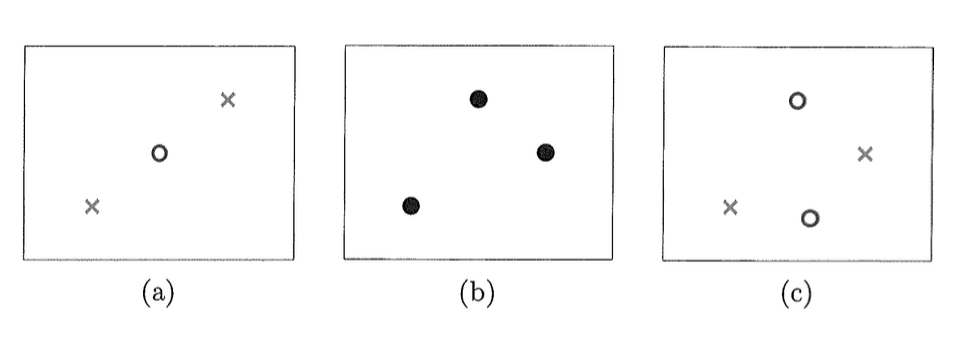
\includegraphics[width=0.8\textwidth]{Images/5.png}
    
    \caption{Fragmentación de muestras en $\mathbb{R}^2$ de tres y cuatro puntos. (Gráfica tomada de [11])}
    \label{fragmentacion perceptron}
    \end{figure}

Es claro que no es posible separar de todas las maneras posibles a esta muestra en particular, por lo que su conjunto de fragmentación
tiene un cardinal menor a $2^3=8$. Pero sí es posible hacerlo con otras muestras de tres elementos, como por ejemplo cualquiera que tenga 
tres puntos no colineales, como en la figura \ref{fragmentacion perceptron} (b). De esto sigue
que los clasificadores lineales de este tipo tienen un coeficiente de fragmentación máximo de $2^3=4$ para muestras de tres puntos en $\mathbb{R}^2$.
Pero notemos que no es así cuando tomamos una muestra de cuatro puntos en $\mathbb{R}^2$. En este caso, es imposible separar de todas las maneras posibles
a una muestra de cuatro puntos, sean colineales o no, como se aprecia en la parte (c) de la figura. Demostraremos estos hechos más adelante.\newline

El coeficiente de fragmentación es una medida de la capacidad de una clase de funciones, es decir, mide 
el tamaño o la \textit{complejidad} de \(\mathcal{F}\) en un sentido particular. Si \(\mathcal{F}\) contiene muchas funciones, entonces 
$\mathcal{N}(\mathcal{F}, n)$ tiende a ser grande. Sin embargo, el coeficiente de fragmentación también tiene en cuenta 
la relación entre \(\mathcal{F}\) y el espacio de entrada de donde provienen los puntos de muestra. Más aún, nos permite asignar un número
finito a cada espacio de clasificadores para cada tamaño de muestras, aún cuando los espacios de funciones sean infinitos. Este número puede
ser en el peor de los casos exponencial en el tamaño de la muestra, pero nos ayudará a pasar del factor $m$, que depende de la cantidad
de funciones en el espacio (en la ecuación \ref{eq: chernoff acotada por m}), a un valor que es finito y, como veremos más adelante,
potencialmente polinómico.\newline

\subsection{Cotas de convergencia uniforme}

Mantenemos la atención sobre la ecuación (\ref{eq:med_unif_riesgo_riesgo_emp}). Dado un espacio de funciones arbitrario, 
posiblemente infinito, ahora queremos analizar la probabilidad 
de que el riesgo empírico difiera significativamente del riesgo verdadero. Con las herramientas anteriores, 
podemos derivar una cota como sigue. Consideremos una muestra de \(2n\) puntos, es decir, un conjunto 
\(Z_{2n}\), donde interpretamos los primeros \(n\) puntos como la muestra original y los otros \(n\) 
puntos como la muestra fantasma.\newline

La idea es reemplazar el supremo sobre \(\mathcal{F}\) en términos de \(R(f)\) y 
\(R_{\text{emp}}(f)\) por un supremo sobre los riesgos empíricos calculados en ambas muestras, es decir, por un expresión
que utilice el supremo sobre \(\mathcal{F}_{Z_{2n}}\). En este espacio, existen a lo sumo $\mathcal{N}(\mathcal{F}, n)<2^{2n}$
funciones distintas, lo que nos permite reemplazar, como indicabamos, el valor potencialmente infinito $m$ por el coeficiente de 
fragmentación. Escribimos:\newline

\[
\begin{aligned}
P\left(\sup_{f \in \mathcal{F}} |R(f) - R_{\text{emp}}(f)| > \varepsilon\right) &\leq 
2P\left(\sup_{f \in \mathcal{F}} |R_{\text{emp}}(f) - R'_{\text{emp}}(f)| > \frac{\varepsilon}{2}\right).\\
& = 2P\left(\sup_{f \in \mathcal{F}_{Z_{2n}}} |R_{\text{emp}}(f) - R'_{\text{emp}}(f)| > \frac{\varepsilon}{2}\right).\\
& \leq 2  \mathcal{N}(\mathcal{F}, n)\cdot \exp\left(\frac{-n\varepsilon^2}{4}\right).
\end{aligned}
\]

Primero, utilizando el argumento de simetrización, como antes. Luego, el supremo puede restringirse a un conjunto finito de funciones
dado que estamos considerando solo los riesgos empíricos sobre dos muestras de tamaño $n$, que consideramos fijas, y de allí igualamos
en el segundo paso. Por último, aplicamos la cota de Chernoff (\ref{eq:Chernoff}), sabiendo que el numero de funciones
posibles $m$ es a lo sumo el coeficiente de fragmentación.\newline

Para formalizar esto, usamos el coeficiente de fragmentación \(\mathcal{N}(\mathcal{F}, 2n)\), que proporciona el número máximo 
de particiones que \(\mathcal{F}\) puede realizar sobre una muestra de \(2n\) puntos. Aplicando el límite de la unión 
y la cota de Chernoff, obtenemos:

\begin{equation} 
    P\left(\sup_{f \in \mathcal{F}} |R(f) - R_{\text{emp}}(f)| > \varepsilon \right) \leq 
    2\mathcal{N}(\mathcal{F}, 2n) \exp\left(-\frac{n\varepsilon^2}{4}\right). \label{eq: cota convergencia coeficiente fragmentacion}
\end{equation}

Esta es una cota de convergencia uniforme que conecta el coeficiente de fragmentación con la probabilidad de 
que el riesgo empírico se desvíe significativamente del riesgo verdadero. Para que la minimización del riesgo 
empírico sea consistente, es suficiente que $\mathcal{N}(\mathcal{F}, n)$ crezca a un ritmo razonablemente lento, por ejemplo, 
polinomialmente en \(n\).\newline

Tomemos $\mathcal{F}_{all}$, el espacio de todos los clasificadores posibles. Es claro que, en este caso, $\mathcal{N}(\mathcal{F}_{all}, n)=2^{2n}$,
pues cualquier muestra de $2n$ puntos puede ser separada de $2^{2n}$ formas posibles. Entonces, la cota de convergencia uniforme para este espacio
es:

\[
P\left(\sup_{f \in \mathcal{F}_{all}} |R(f) - R_{\text{emp}}(f)| > \varepsilon \right) \leq
2\cdot 2^{2n} \exp\left(-\frac{n\varepsilon^2}{4}\right) = 2\exp\left(n\left( 2\log(2) - \frac{n\varepsilon^2}{4}\right)\right).
\]

Que es una expresión que no tiende a $0$ cuando $n$ tiende a infinito. Con lo que sabemos hasta ahora, esto no significa que podamos 
concluir que la minimización del riesgo empírico
usando el espacio de todas las funciones clasificadoras posibles sea inconsistente, dado que la cota de convergencia uniforme anterior
es solo una condicion suficiente. Pero si podemos dar el siguiente resultado para definir una condición necesaria y suficiente para
la consistencia de la minimización del riesgo empírico.
\begin{thm}\label{thm: consistencia ssi}
    La minimización del riesgo empírico es consistente con respecto a un espacio de funciones $\mathcal{F}$ si y solo si
    \[
    \frac{\log\left(\mathcal{N}(\mathcal{F}, n)\right)}{n} \rightarrow 0 \qquad \text{cuando } n \to \infty.
    \]
    
\end{thm}

Demostraremos este teorema, de manera más general, en el siguiente capitulo.

\begin{cor}
    Si $\mathcal{N}(\mathcal{F}, n)$ es polinómica, entonces la minimización del riesgo empírico es consistente con respecto a $\mathcal{F}$.\\
\end{cor}
\begin{cor}
    Si $\mathcal{N}(\mathcal{F}, n)=2^n$, entonces la minimización del riesgo empírico no es consistente con respecto a $\mathcal{F}$. En 
    particular, no es consistente con respecto al espacio de todas los clasificadores posibles $\mathcal{F}_{all}$.
\end{cor}

\subsection{Cotas de generalización}

Es a veces útil reescribir la ecuación (\ref{eq: cota convergencia coeficiente fragmentacion}) de forma inversa. Es decir, en lugar de 
fijar \(\varepsilon\) y 
luego calcular la probabilidad de que el riesgo empírico se desvíe del riesgo verdadero en más de \(\varepsilon\), 
podemos especificar la probabilidad con la que queremos que la cota se cumpla, y luego obtener una afirmación 
que nos indique qué tan cerca podemos esperar que esté el riesgo del riesgo empírico. Es decir, fijamos \(\delta > 0\) 
y resolviendo para \(\varepsilon\). Como resultado, obtenemos que, con una probabilidad al menos \(1 - \delta\), cualquier 
función \(f \in \mathcal{F}\) satisface:

\begin{equation}
    R(f) \leq R_{\text{emp}}(f) + \sqrt{\frac{4}{n} \log(2\mathcal{N}(\mathcal{F}, n)) - \log(\delta)}. \label{eq: cota generalizacion}
\end{equation}
\newline

De la misma manera que antes, podemos usar esta cota para derivar afirmaciones de consistencia. Por ejemplo, 
ahora es evidente que la minimización del riesgo empírico es consistente para la clase de funciones \(\mathcal{F}\) 
si el término \(\log(2\mathcal{N}(\mathcal{F}, 2n))/n\) converge a \(0\) cuando \(n \to \infty\). Una vez más, 
este es el caso si \(\mathcal{N}(\mathcal{F}, 2n)\) crece de manera polinómica con \(n\).\newline

Nótese que la cota (\ref{eq: cota generalizacion}) se cumple para todas las funciones \(f \in \mathcal{F}\). 
Por un lado, esto es una fortaleza 
de la cota, ya que se cumple en particular para la función \(f_n\) que minimiza el riesgo empírico, que es lo que 
buscamos. Además, muchos algoritmos de aprendizaje no minimizan exactamente el riesgo empírico, por lo que la cota 
también se cumple para ellos. Sin embargo, esto también puede interpretarse como una debilidad, ya que, al considerar 
un espacio más grande del necesario, obtenemos una cota menos ajustada de lo que podríamos si solo considerásemos
funciones en el espacio del algoritmo de aprendizaje.\newline

Intentemos obtener una intuición sobre esta cota. Nos dice que si tanto \(R_{\text{emp}}(f)\) como el término 
de raíz cuadrada son pequeños simultáneamente, entonces podemos garantizar que, con alta probabilidad, el 
riesgo (es decir, el error en puntos futuros que aún no hemos visto) será pequeño. Esto puede parecer una 
afirmación sorprendente, sin embargo, no afirma nada imposible. Si usamos una clase de funciones con un 
\(\mathcal{N}(\mathcal{F}, n)\) relativamente pequeño, es decir, una clase de funciones que no puede explicar 
muchas funciones posibles, y luego notamos que usando una función de esta clase podemos explicar los datos muestreados 
del problema en cuestión, entonces es probable que esto no sea una coincidencia y hayamos capturado algunos aspectos 
esenciales del problema. \newline

Por otro lado, si el problema es demasiado difícil de aprender a partir de la cantidad de datos dada, entonces 
descubriremos que, para explicar los datos (es decir, para lograr un \(R_{\text{emp}}(f)\) pequeño), necesitamos 
una clase de funciones que sea tan grande que pueda, en esencia, explicar cualquier cosa. En ese caso, el término 
de raíz cuadrada sería grande. Finalmente, nótese que la dificultad de aprender un problema está completamente 
determinada por si podemos encontrar una clase de funciones adecuada y, por lo tanto, por nuestro conocimiento 
previo sobre él. Incluso si la función óptima es subjetivamente muy compleja, si nuestra clase de funciones 
contiene esa función y pocas o ninguna otra, estamos en una excelente posición para aprender.\\

Existe una gran cantidad de cotas similares a (\ref{eq: cota convergencia coeficiente fragmentacion}) 
y su forma alternativa (\ref{eq: cota generalizacion}). Las diferencias ocurren en 
las constantes, tanto en el coeficiente frente a la exponencial como en su exponente. Las cotas también 
difieren en el exponente de \(\varepsilon\) y en la forma en que miden la capacidad.\newline

\subsection{La dimensión VC}

Hasta ahora hemos definido cotas de generalización en términos del coeficiente de framentación.
Aunque este es útil, a menudo es difícil calcularlo para clases de funciones arbitrarias. Existen otras medidas de capacidad
que son más fáciles de calcular y que proporcionan cotas más ajustadas, con ventajas y desventajas.
Introducimos la más conocida de todas, la llamada \textbf{dimensión VC} (dimensión de Vapnik-Chervonenkis). En pocas palabras,
esta medida intenta caratecterizar el crecimiento del coeficiente de fragmentación a medida que $n$ crece, destilado en un 
solo valor.\newline

Decimos que una muestra \(Z_n\) de tamaño \(n\) es fragmentada por la clase de funciones 
\(\mathcal{F}\) si \(\mathcal{N}(\mathcal{F}, n) = 2^n\). Es decir, \(\mathcal{F}\) puede realizar cualquier separación posible de etiquetas sobre 
los puntos de la muestra. La dimensión VC de \(\mathcal{F}\), denotada como \(\text{VC}(\mathcal{F})\), se define como el tamaño 
máximo de una muestra que puede ser fragmentada por \(\mathcal{F}\). Formalmente:\newline

\begin{dfn}
La dimensión VC de una clase de funciones \(\mathcal{F}\) es el tamaño máximo de una muestra que puede ser fragmentada por \(\mathcal{F}\), es decir:
\[
\text{VC}(\mathcal{F}) = \max \{n \in \mathbb{N} \mid \mathcal{N}(\mathcal{F}, n) = 2^n\}. 
\]
Si no existe tal máximo, definimos \(\text{VC}(\mathcal{F}) = \infty\).\newline
\end{dfn}

La dimensión VC tiene una interpretación combinatoria 
elegante y proporciona una forma práctica de analizar la capacidad de \(\mathcal{F}\). Por ejemplo, si \(\text{VC}(\mathcal{F})\) 
es finita, podemos garantizar la consistencia de la minimización del riesgo empírico. Además, una clase de funciones 
con dimensión VC más baja tiende a tener una mejor capacidad de generalización.\newline

\begin{lem}\label{def:cota combinatoria de dimensión VC}
    Sea $\mathcal{F}$ una clase de funciones con dimensión VC finita. Entonces
    \[
    \mathcal{N}(\mathcal{F}, n) \leq \sum_{i=0}^{\text{VC}(\mathcal{F})} \binom{n}{i} , \qquad \forall n \in \mathbb{N}.
    \]
    En particular, para $n\geq \text{VC}(\mathcal{F})$ se tiene que 
    \[
    \mathcal{N}(\mathcal{F}, n) \leq \left(\frac{e\cdot n}{\text{VC}(\mathcal{F})}\right)^{\text{VC}(\mathcal{F})}.
    \]
\end{lem}

La importancia de esta afirmación radica en el último hecho. Si \( n \geq \text{VC}(\mathcal{F}) \), 
el coeficiente de fragmentación se comporta como una función polinómica del tamaño de la muestra \( n \). 
Este es un resultado muy notable: una vez que sabemos que la dimensión VC de una clase de funciones 
\(\mathcal{F}\) es finita, ya sabemos que los coeficientes de fragmentación crecen polinómicamente con \( n \). 
Por los resultados de la sección anterior, esto implica la consistencia de la minimización del riesgo empírico.\newline

Nótese que también tenemos una afirmación en la otra dirección. Si la dimensión VC es infinita, esto significa 
que para cada \( n \) existe alguna muestra que puede ser fragmentada por \(\mathcal{F}\), es decir, tal que
\(\mathcal{N}(\mathcal{F}, n) = 2^n. \) Para este caso, ya vimos anteriormente que ERM no es consistente.
Enunciamos todo esto en el siguiente Teorema.\newline

\begin{thm}
    La minimización del riesgo empírico es consistente con respecto a una clase de funciones \(\mathcal{F}\) si y solo si
    \(\text{VC}(\mathcal{F}) < \infty\).\newline 
\end{thm}

Una propiedad importante a notar tanto sobre el coeficiente de fragmentación como sobre la 
dimensión VC es que no dependen de la distribución subyacente \( P \), sino únicamente de la 
clase de funciones \(\mathcal{F}\). Por un lado, esto es una ventaja, ya que todas las cotas de 
generalización derivadas de estos conceptos se aplican a todas las distribuciones de probabilidad 
posibles. Por otro lado, esto también puede considerarse una desventaja, ya que los conceptos de 
capacidad no tienen en cuenta propiedades particulares de la distribución en cuestión. En este 
sentido, estos conceptos de capacidad a menudo conducen a cotas bastante amplias, pero es lo que desde
un comienzo nos interesaba.\newline


\chapter{La Teoría VC}

En el capítulo previo, hemos intentado proveer una descripción liviana y en el orden de lo intuitivo de la teoría brindada por 
Vapnik y Chernovenkis. Ahora nos proponemos alcanzar la rigurosidad necesaria para demostrar los teoremas que hemos presentado 
previamente. Para ello, introduciremos una nueva notación y seguiremos [8], el célebre artículo de 1971 - escrito tres años antes en su 
idioma original - por los dos colosos rusos.\newline

\section{Definiciones preliminares}

Sea \( \Omega \) un conjunto de eventos sobre el cual se ha definido una medida de probabilidad \( P \). Sea \( \mathcal{S} \) una colección de eventos 
aleatorios, es decir, subconjuntos del espacio \( \Omega \) que son medibles con respecto 
a la medida \( P \). \newline
\begin{dfn}
    Denotemos por \( \Omega^{(l)} \) el espacio de muestras de tamaño \( l \) en \( \Omega \). Es decir
    \[ \Omega^{(l)} = \underbrace{\Omega \times \Omega \times \ldots \times \Omega}_{l \text{ veces}}. \]
\end{dfn}

\begin{obs}
Los elementos en  \( \Omega^{(l)} \) son muestras de tamaño $l$, por lo que son vectores
aleatorios compuestos por $l$ variables aleatorias independientes e idénticamente distribuídas.
Luego
$$
Z_l = (\omega_1, \ldots, \omega_l)
$$
es un elemento de \( \Omega^{(l)} \).
\end{obs}

\begin{dfn}
Seguiremos las siguientes convenciones:
\begin{enumerate}
    \item $X^{(l)} = (X(\omega),\ldots,X(\omega))$ es un vector aleatorio de tamaño $l$ (es un vector de funciones, todas ellas iguales).
    \item $x^{(l)} = (X(\omega_1),\ldots,X(\omega_l)) \in \mathbb{R}^l$ es la realización vector aleatorio de tamaño $l$ (es un vector en $\mathbb{R}^l$).
    \item $Z_l = (\omega_1,\ldots,\omega_l)$ es una muestra aleatoria (es un conjunto de elementos del espacio muestral $\Omega$).
\end{enumerate}
\end{dfn}

\begin{ej}
    Consideremos la variable aleatoria $X\sim B(p=0.5)$. Un vector aleatorio de tamaño $5$ es
    $$
    X^{(5)} = (X,X,X,X,X),
    $$
    El cual podria realizarse con valores
    $$
    x^{(5)} = (1,0,1,0,0).
    $$
    Estos valores numéricos, corresponden a eventos en el espacio muestral, a los que hemos asignado el valor $1$
    para el éxito y $0$ para el fracaso. Por lo tanto, el elemento de $\Omega^{(l)}$ en este caso es
    $$
    Z_{5}=(\omega_1, \omega_2, \omega_3, \omega_4, \omega_5)
    $$
    donde $\omega_1$ y $\omega_3$ implican éxito, mientras que $\omega_2, \omega_4$ y $\omega_5$ implican fracaso.
\end{ej}

\begin{ej}
    Sea $\Omega$ el espacio muestral, al que definimos como los posibles resultados de lanzar dos monedas no cargadas. Sean $\circ$ (cara) y $+$ (cruz)
    los posibles resultados. Entonces los elementos del espacio muestral son todas las combinaciones posibles de estos resultados:
    $$
        \Omega = \{(\circ,\circ), (\circ,+),(+,\circ),(+,+)\}.
    $$
    Una posible muestra de tamaño $3$ es:
    $$
        Z_{3} = \{(+,\circ),(+,+), (\circ,\circ)\}.
    $$
    Si ahora definimos como \emph{éxito} el sacar al menos una cara en cada evento, el vector aleatoria realizado tendría valores:
    $$
        x^{(3)} = (X(+,\circ), X(+,+), X(\circ,\circ)) = (1,1,0).
    $$
\end{ej}

\begin{dfn}
    Sobre el espacio \( \Omega^{(l)} \), definimos una medida de probabilidad \( P^{(l)} \) tal que

\begin{equation}\label{def: probabilidad en espacio muestral}
P^{(l)}(A_1\times A_2 \times\dots\times A_l) = P(A_1) P(A_2) \dots P(A_l),
\end{equation}
donde los \( A_i \) son subconjuntos medibles de \( \Omega \).\newline
\end{dfn}


\begin{dfn}
Cada muestra \( Z_l = \{\omega_1, \dots, \omega_l\} \) y cada evento \( A \in \mathcal{S} \) determinan 
una \textbf{frecuencia relativa} para \( A \), la cual es igual al cociente entre 
el número \( n_A \) de elementos de la muestra que pertenecen a \( A \) y el tamaño 
total de la muestra:

\[
\nu_A(\{\omega_1,\dots, \omega_l\}) = \nu(A,Z_l) = \frac{n_A(Z_l)}{l} = \frac{\#(\{ \omega_i \in Z_l \mid \omega_i \in A \})}{l}.
\]

\end{dfn}

Observemos que la frecuencia relativa no es más que una frecuencia empírica del evento $A$, es decir, como ese evento
se hace presente en las muestras que tomamos. Rn lo siguiente, representará al riesgo
empírico. 

Un conocido resultado de la relación entre esta probabilidad muestral y la probabilidad real en el espacio
es el Teorema de Bernoulli, el cual es una de las versiones de las leyes de los grandes números que destacamos en el capítulo 1.
\bigskip
\begin{thm}[de Bernoulli]
Sea \( A \in \mathcal{S} \) un evento aleatorio, $P(A)$ la probabilidad del evento $A$ y $\nu_A(\{\omega_1,\dots, \omega_l\})$ su frecuencia relativa para una muestra de
tamaño $l$. Entonces, para cualquier $\varepsilon > 0$,
\[
    \lim_{l\to\infty} P^{(l)}\left(| P(A)-\nu_A(\{\omega_1,\dots, \omega_l\})| \geq \varepsilon\right) = 0.
\]
\end{thm}

Es decir, la frecuencia relativa (o probabilidad empírica) converge en probabilidad (en medida) a la probabilidad real del evento $A$ (la medida de $A$ en $(\Omega, S, P)$).\newline

Nos interesará el supremo de esta diferencia sobre todos los posibles eventos en $\mathcal{S}$:
\begin{equation}
    \pi^{(l)} = \sup_{A\in\mathcal{S}} |P(A)-\nu_A(\{\omega_1,\dots, \omega_l\})|. \label{def: funcion pi}
\end{equation}

Notemos que analizando el comportamiento de la medida de dicho supremo al crecer el tamaño muestral, 
estaremos en condiciones de hacer afirmaciones acerca de la ecuación (\ref{eq:med_unif_riesgo_riesgo_emp}),
que es una instancia particular de esta.\newline

\begin{obs}
$\pi$ es una función puntual en el espacio \( \Omega^{(l)} \). Es decir
\[ \pi(A, \Omega^{(l)}): \Omega^{(l)} \rightarrow \mathbb{R}
\]
Además, supondremos que esta función es medible con respecto a la medida en \( \Omega^{(l)} \), 
es decir, que \( \pi(A, \Omega^{(l)}) \) es una variable aleatoria.
\end{obs} 
\begin{dfn}
Si la variable \( \pi(A, \Omega^{(l)}) \) converge en probabilidad a cero a medida que 
el tamaño de la muestra crece indefinidamente, diremos que la frecuencia relativa 
de los eventos \( A \in \mathcal{S} \) tiende (en probabilidad) a la probabilidad 
de estos eventos de manera \emph{uniforme} sobre la clase \( \mathcal{S} \).
\end{dfn}


Los teoremas siguientes están dedicados a obtener estimaciones para la probabilidad 
de los eventos \( \{ \pi(A, \Omega^{(l)}) > \varepsilon \} \) y a clarificar las condiciones 
bajo las cuales, para cualquier \( \varepsilon \),

\[
\lim_{l \to \infty} P^{(l)}\left\{\pi^{(l)} > \varepsilon\right\} = 0.
\]
\bigskip


\begin{dfn}
Sea \( Z_r = \{\omega_1, \dots, \omega_r\} \) una muestra finita de elementos en \( X \). 
Cada conjunto \( A \) en \( \mathcal{S} \) determina en esta muestra un subconjunto 
\[ 
    Z_l^A = Z_l \cap A = \{\omega_i \in Z_l \mid \omega_i \in A\}, 
\]
que consiste en aquellos elementos de la 
muestra \( Z_l \) que pertenecen a \( A \). Diremos que el conjunto \( A \) \textbf{induce} 
el subconjunto \( Z_l^A  \) en la muestra \( Z_l \).
\end{dfn}
\bigskip

\begin{dfn}
Denotamos el conjunto de todos los subconjuntos diferentes inducidos por los 
conjuntos de \( \mathcal{S} \) en la muestra \( Z_r = \{\omega_1, \dots, \omega_r\} \) como \( \mathcal{S}(\omega_1, \dots, \omega_r) \) 
o \( \mathcal{S}(Z_r) \). Es decir
\[
    \mathcal{S}(Z_r) =  \left\{Z_r^A \mid A \in \mathcal{S}\right\}.
\]
\end{dfn}
\bigskip

\begin{dfn}
El número de subconjuntos distintos de la muestra \( Z_r = \{\omega_1, \dots, \omega_r\} \) 
inducidos por los conjuntos en \( \mathcal{S} \) será denominado el \textbf{índice 
del sistema \( \mathcal{S} \)} con respecto a la muestra \( Z_r \) 
y será denotado por $\Delta^{\mathcal{S}}(Z_r)$. Es decir
\[
\Delta^{\mathcal{S}}(\omega_1, \dots, \omega_r) = \#\left(\mathcal{S}(\omega_1, \dots, \omega_r)\right).
\]
\end{dfn}

Reparemos en que si consideramos los subconjuntos de $\mathcal{S}$ como los posibles conjuntos en
los cuales los clasificadores binarios de un espacio funcional $\mathcal{F}$ pueden etiquetar a los
elementos de $X$, entonces $\Delta^{\mathcal{S}}(Z_r)$ es el cardinal del conjunto de fragmentación $\mathcal{F}_{Z_r}$.
La siguiente observación es también una generalización
de lo que hemos dicho en tanto a la cardinalidad del conjunto de fragmentación.\newline


\begin{obs} El índice del sistema puede ser a lo sumo $2$ elevada a la cantidad de elementos en la muestra. Es decir
\[
    \Delta^{\mathcal{S}}(\omega_1, \dots, \omega_r) \leq 2^r
\]
\end{obs}

Por último, generalizamos la noción de coeficiente de fragmentación en la \textit{función de crecimiento},
tomando el máximo sobre todos los índices posibles.\newline

\begin{dfn}
    Llamaremos \textbf{función de crecimiento} de orden $r$ al índice máximo de un sistema sobre todas las muestras
    posibles de tamaño $r$ sobre un espacio $X$. 
    \[
    m^{\mathcal{S}}(r) = \max_{\{\omega_1,\dots,\omega_r\}}\Delta^{\mathcal{S}}(\omega_1,\dots,\omega_r)
    \]
\end{dfn}
\bigskip

\textbf{Ejemplo 1}: Sea \( \Omega \) una línea recta y sea \( \mathcal{S} \) el conjunto 
de todos los rayos de la forma \( X \leq a \). En este caso, la función de crecimiento es  
\[
m^{\mathcal{S}}(r) = r + 1.
\]

\textbf{Ejemplo 2}: Sea \( \Omega \) el segmento \([0,1]\). El conjunto \( \mathcal{S} \) 
consiste en todos los conjuntos abiertos. En este caso,  
\[
m^{\mathcal{S}}(r) = 2^r.
\]

\textbf{Ejemplo 3}: Sea \( \Omega = E_n \), el espacio euclidiano de dimensión \( n \). 
El conjunto \( \mathcal{S} \) de eventos consiste en todos los semiespacios de la forma  
\[
\langle X_0, \varphi \rangle \geq 1,
\]  
donde \( \varphi \) es un vector fijo y las llaves representan el producto interno en el espacio.
 Evaluemos la función de crecimiento \( m^{\mathcal{S}}(r) \).\newline

Consideremos, junto con el espacio \( E_n \) de vectores \( V \), el espacio \( E_n \) 
de vectores \( \varphi \). A cada vector \( v \in E_n \) le corresponde una partición 
del espacio \( E_n \) en dos subespacios: \(\langle v_k, \varphi_2 \rangle \geq 1\) y \(\langle v_k, \varphi_2 \rangle < 1\). 
Recíprocamente, cada vector \(\varphi\) determina un evento $A$ en el sistema \(\mathcal{S}\).\newline

Tomemos \( r \) vectores \( v_1, \dots, v_r \). Estos generan una partición del espacio \( E_n \) 
en un número de componentes tales que los vectores \( \varphi \) dentro de cada componente determinan eventos 
\( A \in \mathcal{S} \) que inducen el mismo subconjunto en la muestra \( \{\omega_1, \dots, \omega_r \}\).\newline

Este último ejemplo motiva la siguiente definición, que nos será útil en adelante.\newline

\begin{dfn}
    Sea \( \Phi(n, r) \) el número máximo de componentes en los que es posible particionar el espacio \( n \)-dimensional 
mediante \( r \) hiperplanos. Llamaremos a esta función \textbf{función de crecimiento lineal} del sistema.
\end{dfn}


Para el ejemplo 3, por definición:
\[
    m^{\mathcal{S}}(r) = \Phi(n, r).
\]
Es decir, la función de crecimiento lineal es igual a la función de crecimiento cuando solo consideramos partición
del espacio por medio de hiperplanos.

\begin{obs}
Podemos definir a la función de crecimiento lineal en términos recursivos. 
\[
    \Phi(n, r) = \Phi(n, r - 1) + \Phi(n - 1, r - 1),\quad \Phi(0, r) = 1, \quad \Phi(n, 0) = 1.
\]
Esto a su vez nos permite dar la definición combinatoria de la funcion de crecimiento lineal:

\begin{equation}
\Phi(n, r) =
\begin{cases}
\sum\limits_{k=0}^{n} \binom{n}{k}, & \text{si } r > n, \\
2^r, & \text{si } r \leq n.
\end{cases}
\label{def: combinatoria función crecimiento lineal}
\end{equation}
\end{obs}

Por último, observamos que

\begin{obs}   
Para \( n > 0 \) y \( r \geq 0 \), se cumple que:

\[
\Phi(n, r) \leq r^n + 1.
\]

Y tomaremos \( \binom{n}{k} = 0 \) en el caso que \( n < k \).\newline
\end{obs}

\section{La función de crecimiento}

Una propiedad que nos interesa del coeficiente de fragmentación (y por extensión, de la dimensión VC) es que podamos asegurarnos
de que, de ser posible, sean polinómicas. De esa manera la desigualdad (\ref{eq: cota convergencia coeficiente fragmentacion})
es absorvida por la exponencial y nos aseguramos la convergencia en probabilidad. \newline

Ahora probaremos que la función de crecimiento $m^{\mathcal{S}}(r)$ 
es idénticamente igual a \( 2^r \) o está acotada superiormente por \( r^n + 1 \) (es decir, es a lo sumo polinómica),  
donde \( n \) es una constante que corresponde al valor de \( r \) para el cual la igualdad  
\[
m^{\mathcal{S}}(r) = 2^r
\]
se viola por primera vez. Para demostrar este hecho, necesitamos el siguiente lema.\newline

\begin{lem}\label{Lema 1}
Si para alguna muestra  \( \omega_1, \ldots, \omega_i \) de tamaño $i$ y algún número \( n \), con \( 1 \leq n \leq i \),  
se cumple que  
\[
\Delta^{\mathcal{S}}(\omega_1, \ldots, \omega_i) \geq \Phi(n, i),
\]  
entonces existe un subconjunto \( \omega_{i_1}, \dots, \omega_{i_n} \) de esta muestra tal que  
\[
\Delta^{\mathcal{S}}(\omega_{i_1}, \dots,\omega_{i_n}) = 2^n.
\]  

Donde la función \( \Phi(n, i) \) está definida de forma recursiva.  \newline
\end{lem}

Una demostración de este lema puede hallarse en [8].
Ahora si, enunciamos y demostramos el resultado.\newline

\begin{thm} \label{teo: cota polinomica de la función de crecimiento}
    La función de crecimiento \( m^{\mathcal{S}}(r) \) es idénticamente igual a \( 2^r \) o está acotada superiormente por la función potencia  
    \[
    r^n + 1,
    \]
    donde \( n \) es una constante positiva que corresponde al valor de \( r \) para el cual la igualdad  
    \[
    m^{\mathcal{S}}(r) = 2^r
    \]
    se viola por primera vez.    
\end{thm}

\begin{proof}
Ya hemos dicho que \( m^{\mathcal{S}}(r) \leq 2^r \). Supongamos que \( m^{\mathcal{S}}(r) \) no es 
 igual a \( 2^r \) y que \( n \) es el primer valor de \( r \) para el cual \( m^{\mathcal{S}}(r) \neq 2^r \). 
    Entonces, para cualquier muestra de tamaño \( r > n \),
    
    \[
    \Delta^{\mathcal{S}}(\omega_1, \dots, \omega_r) < \Phi(n, r).
    \]
    
    De lo contrario, en base a la afirmación del lema, se podría encontrar una sub muestra  
    \( Z_n^A = \{\omega_i \in Z_n \mid \omega_i \in A\} \) tal que  
    
    \[
    \Delta^{\mathcal{S}}\left(Z_n^A\right) = 2^n.
    \]
    
  Pero esto contradice la suposición inicial de que \( m^{\mathcal{S}}(n) < 2^n \).  
    Así, \( m^{\mathcal{S}}(r) \) es o bien idénticamente igual a \( 2^r \), o bien está acotada superiormente 
    por \( \Phi(n, r) \). A su vez, para \( r > 0 \), se cumple que \( \Phi(n, r) \leq r^n + 1 \) por la observación
    anterior. Sigue que 
    \[
        m^{\mathcal{S}}(r)   \leq r^n + 1.\newline
    \]
    
\end{proof}


Detengámonos un momento en considerar que significan estos resultados en tanto hemos pensado los espacios funcionales
de clasificadores en la sección anterior. Ya hemos dicho que el coeficiente de fragmentación de un espacio para un tamaño
de muestra dada es una instancia de la función de crecimiento. Es decir

\[
\mathcal{N}(\mathcal{F}, r) = m^{\mathcal{S}}(r)
\]

Por otro lado, si $n$ es el primer valor donde la igualdad $m^{\mathcal{S}}(r)=2^r$ se viola, la dimensión VC de un espacio $\mathcal{F}$ 
por definición es $n-1$, es decir el mayor tamaño de muestra que puede ser fragmentado por $\mathcal{F}$.\newline

Considerando la definición combinatoria de la función de crecimiento lineal (\ref{def: combinatoria función crecimiento lineal}),
hemos demostrado el Lema (\ref{def:cota combinatoria de dimensión VC}). Lo enunciamos de forma general en el siguiente corolario.

\begin{cor}
    En las condiciones del teorema anterior, si $n\in\mathbb{N}$ es el mínimo valor del tamaño muestral $r$ tal que    
    \[
        m^{\mathcal{S}}(r) < 2^r
    \]
    entonces
    \[
        m^{\mathcal{S}}(r) \leq \sum\limits_{k=0}^{n} \binom{n}{k}. 
    \]
\end{cor}

\bigskip

\section{El Lema de simetrización}

Enfoquémonos ahora en probar el lema de simetrización (\ref{lema de simetrizacion}). Tomemos dos muestra de tamaño $l$ y
unifiquémolas en una sola muestra de tamaño \( 2l \),
\( Z_{2l} = \{ \omega_1, \dots, \omega_l, \omega_{l+1}, \dots, \omega_{2l} \} \). Supongamos que las frecuencias relativas del evento \( A \in \mathcal{S} \) 
han sido calculadas en la primera semimuestra \( \{ \omega_1, \dots, \omega_l \} \) y en la segunda semimuestra \( \{ \omega_{l+1}, \dots, \omega_{2l} \} \)
por separado.\newline

Para cualquier evento $A\in\mathcal{S}$, denotemos las respectivas frecuencias por \( \nu_A^{(1)}\) y \( \nu_A^{(2)} \), 
y consideremos la diferencia entre estas cantidades:

\[
\rho^{(l)}_A = |\nu_A^{(1)} - \nu_A^{(2)}|.
\]

Nos interesa la máxima diferencia entre estas cantidades sobre todos los eventos en la clase \( \mathcal{S} \),

\[
\rho^{(l)} = \sup_{A \in \mathcal{S}} \rho_A(l).
\]

Observemos que 

\[
\sup_{A \in \mathcal{S}} \rho_A^{(l)} = \max_{A \in \mathcal{S}} \rho_A^{(l)},
\]

ya que, para un \( l \) fijo, \( \rho_A^{(l)} \) solo toma un número finito de valores. Expliquemos esto.
Al fijar dos muestras de tamaño $l$, tenemos a lo sumo $2l$ elementos distintos del espacio $\Omega$. Tomemos un
subconjunto $A\subset \Omega$ tal que $A\in\mathcal{S}$. Para cada muestra $Z_l$, hemos definido la frecuencia muestral
como 

\[
\nu(A,Z_l) = \frac{n(A,Z_l)}{l} = \frac{\#(\{ \omega_i \in Z_l \mid \omega_i \in A \})}{l}.
\]

Si bien los conjuntos $A$ son potencialmente infinitos, podemos separarlos en un número finito de grupos. Basicamente,
aquellos que contienen un elemento de la muestra $Z_l$, aquellos que contienen dos y así hasta aquellos que contienen
los $l$ elementos de la muestra. Es decir, hay $l$ frecuencias posibles para cada muestra (que ya está fija), aún
tomando infinitos $A\in\mathcal{S}$. Por lo tanto, sus diferencias $\rho_A^{(l)}$ también han de serlo.\newline



Mostraremos que si \( \rho^{(l)} \to 0 \) cuando \( l \to \infty \), entonces también \( \pi^{(l)} \xrightarrow{P} 0 \), 
y que las estimaciones de \( \rho^{(l)}\) conducen a estimaciones para \( \pi^{(l)} \). Recordemos que $\pi$ es la diferencia
entre la frecuencia muestral $\nu(A,Z_l)$ y la probabilidad del evento $A$ definida en (\ref{def: funcion pi}).
De ahora en más, supondremos que \( \rho^{(l)} \) es una función medible.\newline

Consideremos las dos muestras $Z^{(1)}_l = \{\omega_1,\dots, \omega_l\}$ y $Z^{(2)}_l = \{\omega_{l+1},\dots, \omega_{2l}\}$.
Es conveniente introducir la siguiente notación:

\[
Q = \left\{ \pi^{(l)} > \varepsilon \right\} = \left\{ \sup_{A\in\mathcal{S}} |P(A)-\nu_A\left(Z^{(1)}_l\right)| > \varepsilon\right\}
\]
\[
\quad C = \left\{ \rho^{(l)} \geq \frac{1}{2}\varepsilon \right\} = \left\{ |\nu_A^{(1)} - \nu_A^{(2)}| \geq \frac{1}{2} \varepsilon\right\}
= \left\{ |\nu_A\left(Z^{(1)}_l\right) - \nu_A\left(Z^{(2)}_l\right)| \geq \frac{1}{2} \varepsilon\right\}.
\]
\bigbreak
El siguiente es exactamente el Lema de simetrización que hemos presentado con anterioridad.\newline

\begin{lem} [de simetrización]
    Sea \( l \geq 2 / \varepsilon^2 \), entonces

    \[
    P^{(2l)}(C) \geq \frac{1}{2} P^{(l)}(Q).
    \]
\end{lem}
\begin{proof}
Por definición
\begin{equation*}
P^{(2l)}(C) = P^{(2l)}\left(\rho^{(l)}-\frac{\varepsilon}{2}\geq 0\right) = \int_{\Omega^{(2l)}} \left( 1 \cdot \chi_{\{\rho^{(l)}-\frac{\varepsilon}{2}\geq 0\}} + 
0 \cdot \chi_{\{\rho^{(l)}-\frac{\varepsilon}{2}< 0\}} \right) dP(\Omega^{(2l)})
\end{equation*}

Donde integramos sobre el espacio muestral de tamaño $2l$ de tal manera que
\begin{equation}
    \Omega^{(2l)} = \Omega_1^{(l)}\times \Omega_2^{(l)}.  \label{def Z2l prod interno}
\end{equation}

Notemos que los elementos de $\Omega^{(2l)}$ son de la forma $ \{\omega_1,\ldots,\omega_l\} \times \{\omega_{l+1},\dots,\omega_{2l}\}$.\newline

Definamos la función indicadora: 
\[
\theta(z)=\begin{cases}
    1 \text{ si } z\geq 0 \\
    0 \text{ si } z< 0
\end{cases}  
\]

con la cual reescribimos la probabilidad de $C$ como
\begin{equation}
P^{(2l)}(C) = \int_{\Omega^{(2l)}} \left( \theta\left(\rho^{(l)}-\frac{\varepsilon}{2}\right)\right) dP(\Omega^{(2l)})
\end{equation}

Descomponiendo como en (\ref{def Z2l prod interno}) al espacio muestral, podemos escribir:

\[
P^{(2l)}(C) = \int_{\Omega_1^{(l)}\times \Omega_2^{(l)}} \left( \theta\left(\rho^{(l)}-\frac{\varepsilon}{2}\right)\right) dP(\Omega^{(2l)})
\]
Y, tomando $P^{(2l)}=P^{(l)}\times P^{(l)} = P_1\times P_2$, por el teorema de Fubini separamos los signos de integración

\[
P^{(2l)}(C) = \int_{\Omega_1^{(l)}} \left( \int_{ \Omega_2^{(l)}}  \theta\left(\rho^{(l)}-\frac{\varepsilon}{2}\right) dP_2\right) dP_1
\]

Ahora, consideremos el subevento $Q$ sobre el espacio muestral $\Omega_1^{(l)}$, es decir aquellas muestras $\hat{Z}_l$ de $l$
elementos en las cuales se verifica la definición de $Q$ que hemos dado:
\[
Q = \left\{ \pi^{(l)} > \varepsilon \right\} = \left\{\hat{Z}_l\in Z^{(l)}:\; 
\sup_{A\in\mathcal{S}}\left|P_A - \nu_A\left(\hat{Z}_l\right)\right| > \varepsilon \right\},
\]

y restringimos la primer integral a este evento
\begin{equation}
P^{(2l)}(C) \geq \int_{Q} \left( \int_{ \Omega_2^{(l)}}  \theta\left(\rho^{(l)}-\frac{\varepsilon}{2}\right) dP_2\right) dP_1. \label{desigualdad P^(2l)(C)}
\end{equation}

Por definición, para cada muestra $\hat{Z}_l$ en $Q$ debe existir algún evento $A_0\in\mathcal{S}$ tal que $|P_{A_0}-\nu_{A_0}\left(\hat{Z}_l\right)|>\varepsilon$.
Para dicho evento, se cumple

\[
\begin{aligned}
    \varepsilon < \left|P_{A_0}-\nu_{A_0}^{(1)}\right| &= \left|\nu_{A_0}^{(1)}-P_{A_0}\right|\\
    & = \left|\nu_{A_0}^{(1)}-\nu_{A_0}^{(2)}+\nu_{A_0}^{(2)}-P_{A_0}\right| \\
    & \leq \left|\nu_{A_0}^{(1)}-\nu_{A_0}^{(2)}\right|+\left|\nu_{A_0}^{(2)}-P_{A_0}\right|,
\end{aligned}
\]
y así
\[
    \varepsilon - \left|\nu_{A_0}^{(2)}-P_{A_0}\right| < \left|\nu_{A_0}^{(1)}-\nu_{A_0}^{(2)}\right|.
\]\newline
Por lo tanto, la desigualdad
\[
\rho_{A_0}^{(l)} = |\nu^{(1)}_{A_0}-\nu^{(2)}_{A_0}| \geq \frac{\varepsilon}{2},
\]

se verifica si 

\[
|\nu^{(2)}_{A_0}-P_{A_0}|\geq \frac{\varepsilon}{2}.
\]

Retomando la desigualdad (\ref{desigualdad P^(2l)(C)}), reparemos un momento en la integral interior. 
Dada la monotonía de $\theta$ y quedándonos
con tan solo un evento $A_0\in\mathcal{S}$, en vez de tomar el supremo sobre todos los eventos, podemos escribir

\[
\begin{aligned}
\int_{ \Omega_2^{(l)}} \theta\left(\rho^{(l)}-\frac{\varepsilon}{2}\right) dP_2 \;&\geq\; \int_{ \Omega_2^{(l)}}  \theta\left(\rho^{(l)}_{A_0}-\frac{\varepsilon}{2}\right) dP_2 \\
& = \; \int_{ \Omega_2^{(l)}}  \theta\left(\frac{\varepsilon}{2} - |\nu^{(2)}_{A_0}-P_{A_0}|\right) dP_2
\end{aligned}
\]

En donde en la última igualdad aplicamos lo recién explicado. Ahora notemos que 

\begin{equation}\label{eq: theta como probabilidad}
    \int_{ \Omega_2^{(l)}}  \theta\left(\frac{\varepsilon}{2} - |\nu^{(2)}_{A_0}-P_{A_0}|\right) dP_2 \;=\; 1 - P\left(|\nu^{(2)}_{A_0}-P_{A_0}|>\frac{\varepsilon}{2}\right),
\end{equation}


dada la propia definición de $\theta$, que vale $0$ sólo cuando se da la desigualdad dentro de la probilidad de la derecha. Ahora procedemos a acotar dicha probabilidad.\newline

Haciendo uso de la desigualdad de Chebyshev: 
\[
P\left\{|X- \mathbb{E}\left(X \right)| \geq k \cdot \sqrt{\text{Var}(X)} \right\} \leq \frac{1}{k^2}
\]

para la variable aleatoria $X=\nu_{A_0}^{(2)}$ y el valor
\[
k= \frac{\varepsilon}{2\cdot\sqrt{\text{Var}\left(\nu_{A_0}^{(2)}\right)}}   ,
\]

escribimos

\begin{equation}
P\left(|\nu_{A_0}^{(2)} - \mathbb{E}\left(\nu_{A_0}^{(2)} \right)| \geq \frac{\varepsilon}{2}\right) 
\;\leq\; \frac{4}{\varepsilon^2}\cdot \text{Var}\left(\nu_{A_0}^{(2)}\right). \label{Chebyshev aplicada a frecuencia relativa}
\end{equation}
\bigskip

Analicemos esta última desigualdad, factor a factor.\newline

Podemos escribir la frecuencia relativa del evento $A_0$ sobre una muestra $Z_l''=\{\omega_1,\ldots,\omega_l\}$ en el espacio muestral $\Omega^{(l)}_2$ como la suma de variables aleatorias
Bernoulli $\tilde{X}_i$ con $i=1,2,\dots,l$ tales que

\[
    \tilde{X}_i = \begin{cases} 1 \text{ si } X\in A_0\\
        0 \text{ si } X\notin A_0
\end{cases}
\]

donde

\[
    \nu_{A_0}^{(2)} = \frac{1}{l}\sum_{i=1}^l \tilde{X}_i.
\]

Es decir, la frecuencia relativa es una combinación lineal de variables Bernoulli, cada una con probabilidad $P_{A_0}$ (que no es ni mas ni
menos que la probabilidad de que cada muestra esté dentro del evento $A_0$).\newline

Previamente, llamamos $n_{A_0}^{(2)}$ a esta suma, y utilizándola podemos escribir la esperanza de la frecuencia relativa como:

\[
\begin{aligned}
    \mathbb{E}\left(\nu_{A_0}^{(2)} \right) &= \mathbb{E}\left(\frac{n_{A_0}^{(2)}}{l} \right) =  \frac{1}{l} \cdot \mathbb{E}\left( \#\left\{X_i\in Z_l''\mid X_i\in A_0\right\}\right)\\
    &= \frac{1}{l} \cdot l \cdot P_{A_0} = P_{A_0}
\end{aligned}
\]

Que es lo esperable, dado que las muestras en promedio deberian tender a las probabilidades.\newline

Ahora, centrémonos en la varianza de la desigualdad (\ref{Chebyshev aplicada a frecuencia relativa}). Primero,
recordemos que la varianza de toda variable aleatoria Bernoulli tiene forma

\[
     \text{Var}(X) = p(1-p), \qquad X \sim \text{Bernoulli } (p=P(X)).
\]
\bigskip

Esto nos permite escribir la varianza de la frecuencia muestral $\nu_{A_0}$ en términos de la probabilidad del evento $A_0$:

\[
\begin{aligned}
    \text{Var}\left(\nu_{A_0}^{(2)}\right) &=\text{Var}\left(\frac{1}{l}\sum_{i=1}^l \tilde{X}_i\right)
    = \frac{1}{l}\sum_{i=1}^l \text{Var}\left(\tilde{X}_i\right)\\
    &= \frac{1}{l}\sum_{i=1}^l \left[P(\tilde{X}_i)(1-P(\tilde{X}_i))\right]\\
    &=\frac{1}{l} \cdot l\cdot P(\tilde{X}_i)(1-P(\tilde{X}_i)) \\
\end{aligned}
\]

Ahora, como $P(\tilde{X}_i) = P_{A_0}$, tenemos que 
\[
    \text{Var}\left(\nu_{A_0}^{(2)}\right) = P_{A_0}(1-P_{A_0}).
\]

Por lo tanto, podemos reescribir (\ref{Chebyshev aplicada a frecuencia relativa}) como:

\[
P\left( \left| \nu^{(2)}_{A_0} - P_{A_0} \right| > \frac{\varepsilon}{2} \right) 
\leq \frac{4(1 - P_{A_0}) P_{A_0}}{\varepsilon^2 l}.
\]\newline

Dado que $P_{A_0}$ es una probabilidad, y que la función $f(x)=x(1-x)$ tiene un máximo en $x=\frac{1}{2}$, tenemos que
$(1 - P_{A_0}) P_{A_0} \leq \frac{1}{4}$. Por lo tanto,
\[4(1 - P_{A_0}) P_{A_0} \leq 1, 
\]

luego

\[
P\left( \left| \nu^{(2)}_{A_0} - P_{A_0} \right| > \frac{\varepsilon}{2} \right) \leq \frac{1}{\varepsilon^2 l}.
\]\newline

Retomando (\ref{eq: theta como probabilidad}), tenemos 
\[
    \int_{ \Omega_2^{(l)}}  \theta\left(\frac{\varepsilon}{2} - |\nu^{(2)}_{A_0}-P_{A_0}|\right) dP_2 \;\geq\; 1 - \frac{1}{\varepsilon^2 l}.
    \]

Por lo tanto, para \( l \geq 2 / \varepsilon^2 \),

\[
\int_{\Omega_2^{(l)}} \theta \left( \frac{\varepsilon}{2} - \left| \nu^{(2)}_{A_0} - P_{A_0} \right| \right) dP_2 \geq \frac{1}{2}.
\]

De esto se sigue inmediatamente que, para \( l \geq 2 / \varepsilon^2 \),

\[
P^{(2l)}(C) \geq \int_{Q} \left( \frac{1}{2} \right) dP_1  =
 \frac{1}{2} \int_{Q} dP_1.
\]
Por otro lado, podemos escribir
\begin{equation*}
 \begin{split}
   \int_{Q}dP_1 & = \frac{1}{2} \int_{\Omega_1^{(l)}} \chi_{\{Q\}}dP_1 \\
   &=\frac{1}{2}  \int_{\Omega_2^{(l)}}\left(\int_{\Omega_1^{(l)}} \chi_{\{Q\}}dP_1\right) dP_2 \\
   &=\frac{1}{2}  \int_{\Omega_1^{(l)}\times\Omega_2^{(l)}}  \chi_{\{Q\times \Omega_2^{(l)}\}} dP(\Omega^{(2l)}) \\
   &=\frac{1}{2}  P^{(l)}(Q)
\end{split}   
\end{equation*}

Y el lema queda demostrado.\



\end{proof}







Utilizamos el Lema de Simetrización para probar el siguiente teorema.\newline

\begin{thm}
    La probabilidad de que la frecuencia relativa de al menos un evento $A$ en la clase \( \mathcal{S} \) difiera de su probabilidad en una 
    muestra de tamaño \( l \) por más de \( \varepsilon \), para \( l \geq 2 / \varepsilon^2 \), satisface la desigualdad  

    \[
    P^{(2l)}\left(\pi^{(l)} > \varepsilon\right) \leq 4 \; m^{\mathcal{S}}(2l) \; e^{-\varepsilon^2 l/8}.
    \]  
\end{thm}

\begin{proof}
 
En virtud del Lema de Simetrización, basta con estimar  
    
\[
P^{(2l)}\left( \rho^{(l)} \geq \frac{\varepsilon}{2} \right) = \int_{\Omega^{(2l)}} \theta \left( \rho^{(l)} - \frac{\varepsilon}{2} \right) dP(\Omega^{(2l)}).
\]

donde \( \rho^{(l)} \) se considera como una función de la muestra  

\[
\Omega^{(2l)} = (\omega_1, \dots, \omega_l, \omega_{l+1}, \dots, \omega_{2l}),
\]

y $\theta$ es la función indicadora usada en la demostración anterior.\newline

Consideremos la aplicación del espacio \( \Omega^{(2l)} \) sobre sí mismo, resultante de alguna permutación \( T_i \) de los elementos de la muestra \( \Omega^{(2l)} \). Dada la simetría 
de la definición (\ref{def: probabilidad en espacio muestral}) de la medida \( P \) en \( \Omega^{(2l)} \), se cumple la siguiente relación para cualquier función integrable \( f \)
-verifica el Teorema de Fubini- sobre cualquier muestra $Z_{2l}$:

\begin{equation*}
    \begin{split}
            \int_{\Omega^{(2l)}} f(Z_{2l}) \, dP(\Omega^{(2l)}) &= \int_{\Omega_1} \ldots \int_{\Omega_{2l}} f(\omega_1,\ldots,\omega_{2l})  \, d\omega_1\ldots d\omega_{2l} \\
                &= \int_{\Omega_{j_1}}\ldots\int_{\Omega_{j_{2l}}} f(\omega_{j_1},\ldots,\omega_{j_{2l}}) \, d\omega_{j_1}\ldots \omega_{j_{2l}}\\
                &= \int_{\Omega^{(2l)}} f(T_i Z_{2l}) \, dP(\Omega^{(2l)}).
    \end{split}
\end{equation*}

donde $\omega_{j_1},\ldots,\omega_{j_{2l}}$ es una permutación cualquiera de la muestra original, es decir:
\[
T_i Z_{2l} = T_i (\omega_1,\ldots,\omega_{2l}) = \omega_{j_1},\ldots,\omega_{j_{2l}}
\]

lo que implica, en general que:
\[
\int_{\Omega^{(2l)}} f(Z_{2l}) \, dP(\Omega^{(2l)}) = \int_{\Omega^{(2l)}} f(T_i Z_{2l}) \, dP(\Omega^{(2l)}).
\]

Por lo tanto,

\begin{equation}\label{eq:probabilidad integral con permutaciones}
P^{(2l)}\left( \rho^{(l)} \geq \frac{\varepsilon}{2} \right) = \int_{\Omega^{(2l)}} \frac{1}{(2l)!} \sum_{i=1}^{(2l)!} \theta \left( \rho^{(l)}(T_i Z_{2l}) - \frac{\varepsilon}{2}  \right) dP(\Omega^{(2l)}).
\end{equation}

donde simplemente promediamos sobre las \((2l)!\) permutaciones posibles. Notemos que la sumatoria de \((2l)!\) elementos iguales
es igual al valor del elemento por \((2l)!\), por lo que solo multiplicamos y dividimos por este numero lo que se halla dentro de la integral. \newline

Observemos además que

\[
\theta \left( \rho^{(l)} - \frac{\varepsilon}{2} \right) = \theta \left( \sup_{A \in \mathcal{S}} \left| \nu^{(1)}_A - \nu^{(2)}_A \right| -
 \frac{\varepsilon}{2} \right) = \sup_{A \in \mathcal{S}} \theta \left( \left| \nu^{(1)}_A - \nu^{(2)}_A \right| - \frac{\varepsilon}{2} \right).
\]

Claramente, si dos conjuntos \( A_1 \) y \( A_2 \) inducen la misma submuestra en una muestra 

\[
Z_{2l} = (\omega_1, \dots, \omega_l, \omega_{l+1}, \dots, \omega_{2l}),
\]

entonces

\[
\nu^{(1)}_{A_1}(T_i Z_{2l}) = \nu^{(1)}_{A_2}(T_i Z_{2l}), \qquad \nu^{(2)}_{A_1}(T_i Z_{2l}) = \nu^{(2)}_{A_2}(T_i Z_{2l}).
\]

Es decir, tienen idéntica frecuencia muestral relativa, para ambas muestras $(1)$ y $(2)$. Por lo tanto, las diferencias entre cada una de estas frecuencias también serán idénticas

\[
\rho^{(l)}_{A_1}(T_i Z_{2l}) = \rho^{(l)}_{A_2}(T_i Z_{2l}),
\]

para cualquier permutación \( T_i \). Esto implica que si elegimos el subsistema \( \mathcal{S}' \subseteq \mathcal{S} \)
 que consiste en todos los conjuntos \( A \) que inducen submuestras esencialmente diferentes en la muestra \( Z_{2l} \),
el valor del siguiente supremo no cambiará al tomarlo sobre la restricción $S'$:

\[
\sup_{A \in \mathcal{S}} \theta \left( \rho^{(l)}_A(T_i Z_{2l}) - \frac{\varepsilon}{2} \right) = 
\sup_{A \in \mathcal{S}'} \theta \left( \rho^{(l)}_A(T_i Z_{2l}) - \frac{\varepsilon}{2} \right) 
\]

A su vez, podemos acotar la expresión por la suma sobre un numero finito de eventos, los que nos permite escribir

\[
\sup_{A \in \mathcal{S}} \theta \left( \rho^{(l)}_A(T_i Z_{2l}) - \frac{\varepsilon}{2} \right)
\leq \sum_{A \in \mathcal{S}'} \theta \left( \rho^{(l)}_A(T_i Z_{2l}) - \frac{\varepsilon}{2} \right).
\]

Notemos que este es exactamente el mismo argumento que utilizamos en el capítulo anterior para acotar la medida de probabilidad del supremo de la diferencia
entre el riesgo y el riesgo empírico, tomado sobre todos los clasificadores en un espacio funcional, utilizando solo una cantidad finita de clasificadores en el espacio.
Recordemos que llamamos indíce del sistema al cardinal del conjunto $S'$, al que notamos como $ \Delta^{\mathcal{S'}}(\omega_1, \dots, \omega_{2l})$.\newline

Ahora, podemos acotar la integral en (\ref{eq:probabilidad integral con permutaciones}) escribiendo
\[
\frac{1}{(2l)!} \sum_{i=1}^{(2l)!} \theta \left(  \rho^{(l)}(T_i Z_{2l}) - \frac{\varepsilon}{2}  \right) 
= \frac{1}{(2l)!} \sum_{i=1}^{(2l)!} \sup_{A \in \mathcal{S}} \theta \left(  \rho^{(l)}_A(T_i Z_{2l}) - \frac{\varepsilon}{2}  \right)
\]

\[
\leq \sum_{A \in \mathcal{S}'} \left[ \frac{1}{(2l)!} \sum_{i=1}^{(2l)!} \theta \left(  \rho^{(l)}_A(T_i Z_{2l}) - \frac{\varepsilon}{2}  \right) \right].
\]

La expresión entre corchetes denota el cociente del número de permutaciones para una muestra fija 
para las cuales \( |\nu^{(1)}_A - \nu^{(2)}_A| \leq \frac{1}{2} \varepsilon \) y el número total de posibles permutaciones, $(2l)!$. Esta expresión
es exactamente igual a:

\[
\Gamma = \sum_{k : |2\frac{k}{l} - \frac{n_A}{l}| \geq \frac{\varepsilon}{2}} \frac{\binom{n_A}{k} \binom{2l - n_A}{l - k}}{\binom{2l}{l}}.
\]

donde \( n_A \) es el número de elementos en la muestra \( \{\omega_1, \dots, \omega_{2l}\} \) que pertenecen a \( A \), como ya hemos dicho. \newline 

Esta expresión satisface la estimación 

\[
\Gamma \leq 2 e^{-\varepsilon^2 l / 8},
\]

que se obtiene mediante un cálculo sencillo pero largo y cuya demostración puede hallarse en la página 163 de [3], junto con una explicación de la propia función $\Gamma$.  \newline

Por lo tanto,
\begin{equation}\label{promedio de tita acotado por la funcion de crecimiento}
\begin{aligned}
\frac{1}{(2l)!} \sum_{i=1}^{(2l)!} \theta \left(  \rho^{(l)}(T_i Z_{2l}) - \frac{\varepsilon}{2} \right) 
&\leq \sum_{A \in \mathcal{S}'} 2 e^{-\varepsilon^2 l / 8} \\
&= 2 \Delta^{\mathcal{S}}(\omega_1, \dots, \omega_{2l}) e^{-\varepsilon^2 l / 8}\\
&\leq 2 m^S(2l) e^{-\varepsilon^2 l / 8}.
\end{aligned}
\end{equation}

Integrando a cada lado, donde el derecho implica la integral de una constante, y aplicando el Lema de Simetrización, tenemos
\[
P^{(2l)}\left(\pi^{(l)}>\varepsilon\right) \leq 2 P^{(l)}(Q) \leq 2 \cdot 2 m^S(2l) e^{-\varepsilon^2 l / 8}.
\]

\end{proof}

El siguiente corolario es inmediato y nos dice una condición suficiente para que las frecuencias relativas de 
los eventos en la clase \( \mathcal{S} \) converjan uniformemente sobre \( \mathcal{S} \) (en probabilidad) a sus 
correspondientes probabilidades.

\begin{cor}
En las condiciones del teorema anterior, supongamos que existe un $n$ finito tal que:
\[
m^{\mathcal{S}}(l) \leq l^n + 1, \quad \text{para todo } l.
\]
entonces
\[
\lim_{l\to\infty} P^{(l)}\left(Q\right)= 0.
\]
\end{cor}

\begin{proof}

Retomando las condiciones de la demostración anterior, sea $l=2k$
\[
m^S(2k)<(2k)^n + 1
\]

por la cota dada en el Teorema (\ref{teo: cota polinomica de la función de crecimiento}), lo que nos da
\[
\lim_{k\to\infty} P^{(2k)}\left(\pi^{(2k)}>\varepsilon\right) \leq 4 \lim_{l\to\infty} ((2k)^n+1) e^{-\varepsilon^2 k / 8} = 0.
\]    
\end{proof}


\bigskip
Hemos dado condiciones suficientes para que las frecuencias relativas (nuestras probabilidades empíricas) converjan uniformemente a las 
probabilidades reales de los eventos en la clase \( \mathcal{S} \). En la siguiente sección veremos que estas condiciones nos aseguran, además, 
convergencia uniforme de forma casi segura.\newline

\section{Condiciones de convergencia uniforme casi segura}

Comenzamos demostrando el siguiente lema, bien conocido en la teoría de probabilidades, y una consecuencia directa del primer lema de Borel Cantelli \ref{primer lema de Borel-Cantelli}.

\begin{lem}\label{Aplicacion del lema de Borel-Cantelli}
    Sea $\{\xi_i\}_{i\in\mathbb{N}}$ una sucesión de variables aleatorias y $a\in\mathbb{R}$. Si para cualquier \( \varepsilon > 0 \),

    \[
    \sum_{i}^{\infty} P(|\xi_i - a| > \varepsilon) < \infty,
    \]
    
    entonces,
    
    \[
    P(\xi_i \to a) = 1.
    \]
\end{lem}

\begin{proof}
    Sea $\varepsilon > 0$. Sea el evento
    \[
        A_i = \{ \omega \in \Omega : |\xi_i(\omega)-a| > \varepsilon\}.
    \]
Por nuestra hipótesis,
\[
    \sum_{i=1}^{\infty}P(A_i) < \infty,
\]
por lo que el primer lema de Borel-Cantelli nos permite asegurar que
\[
    P\left( \limsup_i A_i \right) = 0.
\]

Esto no es más que
\[
P\left( \bigcap_{n=1}^{\infty} \bigcup_{i\geq n}^{\infty} \{ \omega \in \Omega : |\xi_i(\omega)-a| > \varepsilon\} \right) = 0.
\]

Lo que implica que el evento $A_i$ sucede infinitamente con probabilidad cero. Nos interesa la probabilidad del evento complementario

\[
P(A_i^c) = P(\{ \omega \in \Omega : |\xi_i(\omega)-a| < \varepsilon\}).
\]
Recordando que
\[
\left(\limsup_i A_i\right)^c = \liminf_i A_i^c
\]
tenemos
\[
P\left(\liminf_i A_i^c\right) = P\left(\left(\limsup_i A_i\right)^c\right) = 1 - P\left( \limsup_i A_i \right) = 1.
\]
Como la probabilidad de cualquier evento es a lo sumo uno: 
\[
1 = P\left(\liminf_i A_i^c\right) \leq P\left(\lim_i A_i^c\right) \leq P\left( \limsup_i A_i^c \right) \leq 1,
\]
por lo que 
\[
P\left(\lim_i A_i^c\right) = P(\xi_i \to a) = 1.
\]
\end{proof}

\begin{thm}
    Si \( m^{\mathcal{S}}(l) \leq l^n + 1 \), entonces  

    \[
    P^{(l)}(\pi^{(l)} \to 0) = 1.
    \]
    
\end{thm} 

\begin{proof}

Dado que  

\[
P^{(l)}(\pi^{(l)} > \varepsilon) \leq 4 m^{\mathcal{S}}(2l)  e^{-\varepsilon^2 l/8},
\]

para \( l \geq 2 / \varepsilon^2 =L \), la serie  

\[
\sum_{l=1}^{\infty} P^{(l)}(\pi^{(l)} > \varepsilon) \leq \sum_{l=1}^{L} P^{(l)}(\pi^{(l)} > \varepsilon) + 4 \sum_{l=L+1}^{\infty} [(2l)^n + 1] e^{-\varepsilon^2 l/8}
\]

es convergente para cualquier \( \varepsilon \).  \newline

Por el lema \ref{Aplicacion del lema de Borel-Cantelli}, esto implica que  

\[
P^{(l)}(\pi^{(l)} \to 0) = 1.
\]
\end{proof}

\begin{obs}\label{obs:desigualdad triangular indice de un sistema}
    La definición del índice implica inmediatamente que  

    \begin{equation*}
    \Delta^{\mathcal{S}}(\omega_1, \dots, \omega_{k}, \omega_{k+1}, \dots,\omega_l) \leq \Delta^{\mathcal{S}}(\omega_1, \dots, \omega_k) \Delta^{\mathcal{S}}(\omega_{k+1}, \dots, \omega_l).
    \end{equation*}
    De aquí se sigue que  
    \begin{equation*}
    \log_2 \Delta^{\mathcal{S}}(\omega_1, \dots, \omega_{k}, \omega_{k+1}, \dots,\omega_l) \leq \log_2 \Delta^{\mathcal{S}}(\omega_1, \dots, \omega_k) + \log_2 \Delta^{\mathcal{S}}(\omega_{k+1}, \dots, \omega_l).
    \end{equation*}\newline
\end{obs}


En lo que sigue, se asumirá que el índice \( \Delta^{\mathcal{S}}(\omega_1, \dots, \omega_l) \), visto como una función de 
\( Z_l = \{\omega_1, \dots, \omega_l\} \), es medible con respecto a la medida \( P \).\newline

\begin{dfn}
    Sean  
    \[
    F^{\mathcal{S}}(z) = P^{(l)}\left(\log_2 \Delta^{\mathcal{S}}(\omega_1, \dots, \omega_l) < z \right).
    \]
     
    \[
    H^{\mathcal{S}}(l) = \mathbb{E} \left[ \log_2 \Delta^{\mathcal{S}}(\omega_1, \dots, \omega_l) \right].
    \]

    Llamamos \textbf{entropía del sistema} de eventos \( \mathcal{S} \) en muestras de tamaño \( l \) a  $H^{\mathcal{S}}(l)$.\newline

\end{dfn}

\begin{obs} \label{subaditividad de la entropia 1}
    Dada la monotonía de la esperanza, la observación (\ref{obs:desigualdad triangular indice de un sistema}) implica que  
    
    \[
        H^{\mathcal{S}}(l_1 + l_2) \leq H^{\mathcal{S}}(l_1) + H^{\mathcal{S}}(l_2).
    \]
\end{obs}

\begin{obs} \label{subaditivdad de la entropia 2}
    Usando la desigualdad anterior de manera repetida obtenemos que, para $k\in \mathbb{N}$:
        \[
        H^{\mathcal{S}}(kl) \leq k H^{\mathcal{S}}(l)
    \]
\end{obs}

Los siguientes lemas nos ayudarán para probar el último de los resultados de este capítulo.\newline

\begin{lem}\label{lema 3}
    La sucesión \( \frac{H^{\mathcal{S}}(l)}{l} \) tiene un límite \( c \), con \( 0 \leq c \leq 1 \), cuando \( l \to \infty \).
\end{lem}
    
\begin{proof}
    Notemos primero que la propia definición de la entropía $H^S$
    \[
    H^S(l) = \mathbb{E}\log_2 \Delta^S(\omega_1,\ldots,\omega_l)
    \] 
    junto a la cota del índice del sistema $S$ en la muestra:
    \[
    1 \leq \Delta^S(\omega_1,\ldots,\omega_l) \leq 2^l
    \]
    nos permiten escribir
    \[
    \log_2 \mathbb{E} (1) \leq H^S(l) \leq \log_2 \mathbb{E} \left(2^l\right),
    \]
    es decir, al dividir por el tamaño de la muestra $l$:
    \begin{equation} \label{cota de la entropia}
        0 \leq \frac{H^S(l)}{l} \leq 1.
    \end{equation}
    Siendo así, sabemos que existe una cota inferior para el límite
    \[
    c = \liminf_{l\to\infty} \frac{H^S(l)}{l}
    \]
    con $c\in [0,1]$.

    Entonces, para cualquier $\varepsilon>0$, existe $l_0\in\mathbb{N}$ tal que
    \begin{equation}\label{cota inferior mas epsilon de la entropia}
        \frac{H^S(l)}{l} < c + \varepsilon, \qquad \forall l \geq l_0.
    \end{equation}
    Observemos que cualquier $l$ puede ser escrito de la forma
    \[
        l = n l_0 + k,
    \]
    con $n\geq 0$ y $k<l_0$, con $k$ positivo. Usando las desigualdades (\ref{subaditividad de la entropia 1}) 
    y (\ref{subaditivdad de la entropia 2}), escribimos
    \begin{equation*}
        H^S(l) = H^S(nl_0+k) \leq nH^S(l_0) + H^S(k) \leq nH^S(l) + k.
    \end{equation*}
    Dividiendo a cada lado por $l=nl_0+k$ tenemos
    \[
        \frac{H^S(l)}{l} \leq \frac{nH^S(l_0) + k}{nl_0+k} < \frac{nH^S(l_0) + l_0}{nl_0} = \frac{H^S(l_0)}{l_0} + \frac{1}{n}.
    \]
    Entonces, por la condición \ref{cota inferior mas epsilon de la entropia}, tenemos
    \[
    \frac{H^S(l)}{l} < c + \varepsilon + \frac{1}{n}.
    \]

    En la medida que $l$ tiende a infinito, $n$ también lo hace. Así
    \[
        \limsup_{l\to\infty} \frac{H^S(l)}{l} < c + \varepsilon
    \]
y dado que $\varepsilon$ es arbitrariamente pequeño
    \[
        \lim_{l\to\infty} \frac{H^S(l)}{l} = c, \qquad 0\leq c\leq 1.
    \]
\end{proof}

En esta demostración hemos probado también que el límite de $c$ es siempre acotado por $\frac{H^S(l)}{l}$ para cualquier $l$ finito.
En efecto, hemos visto que
\[
    \frac{H^S(l)}{l} \leq \frac{H^S(l_0)}{l_0} + \frac{1}{n}
\]
si $l=n l_0+k$. Entonces, para cualquier $\varepsilon>0$ existe un $n_0$ tal que, para todo $n>n_0$, la desigualdad
\[
    \frac{H^S(l)}{l} \leq \frac{H^S(l_0)}{l_0} + \frac{1}{n} + \varepsilon
\]
se verifica. Dejando fijo $l_0$ y tomando el límite sobre $n$ también obtenemos el límite sobre $l$, es decir
\[
    \lim_{l\to\infty} \frac{H^S(l)}{l} \leq \lim_{n\to\infty} \frac{H^S(l_0)}{l_0} + \frac{1}{n} = \frac{H^S(l_0)}{l_0}.
\]
Enunciamos este resultado en el siguiente corolario:

\begin{cor}\label{corolario de la cota del límite de la entropia}
    Para cualquier $l_0$,
    \[
        \frac{H^S(l_0)}{l_0} \geq \lim_{l\to\infty} \frac{H^S(l)}{l} = c.
    \]
\end{cor}

Ahora mostraremos que, para valores grandes de \( l \), la distribución de la variable aleatoria  

\[
\xi^{(l)} = \frac{1}{l} \log_2 \Delta^{\mathcal{S}}(\omega_1, \dots, \omega_l)
\]

se concentra cerca de \( c \). Para esto, usaremos el siguiente resultado.

\bigskip
\begin{lem} \label{lema 4}
    Sea la variable aleatoria
    \[
        \xi^{(l)} = \frac{1}{l} \log_2 \Delta^{\mathcal{S}}(\omega_1, \dots, \omega_l).
    \]

    Entonces
    
    \[
    \lim_{l \to \infty} P^{(l)}(|\xi^{(l)} - c| > \varepsilon) = 0, \quad \text{para } \varepsilon > 0.
    \]
\end{lem}
\bigskip
\begin{proof}
    Denotemos 
    \[ P^{(l)}(l, \varepsilon) = P^{(l)}(|\xi^{(l)} - c| > \varepsilon) , \] 
    \[ P^+(l, \varepsilon) = P^{(l)}(\xi^{(l)} - c > \varepsilon) , \] 
    \[ P^-(l, \varepsilon) = P^{(l)}(c - \xi^{(l)} > \varepsilon) . \]

    En consecuencia,
    
    \[
    P(l, \varepsilon) = P^+(l, \varepsilon) + P^-(l, \varepsilon).
    \]
    
    Observemos que el Lema (\ref{lema 3}) implica la existencia de un \( l_0 \) tal que
    
    \begin{equation}\label{desigualdad 14}
    \left| \frac{H^{\mathcal{S}}(l_0)}{l_0} - c \right| < \frac{\varepsilon}{4}.
    \end{equation}
    
    Estimemos entonces \( P^+(l, \frac{\varepsilon}{2}) \) con \( l = nl_0 \) (siendo \( n \) un entero). Definimos
    
    \[
    y(\omega_1,\ldots,\omega_l) = \frac{1}{nl_0} \sum_{i=0}^{n-1} \log_2 \Delta^{\mathcal{S}}(\omega_{il_0+1}, \dots, \omega_{(i+1)l_0})
    \]
    y observamos que
    \[
    \sum_{i=0}^{n-1} \log_2 \Delta^{\mathcal{S}}(\omega_{il_0+1}, \dots, \omega_{(i+1)l_0})
    \]
    es una suma de variables aleatorias independientes e idénticamente distribuidas, cada una de ellas con esperanza \( H^{\mathcal{S}}(l_0) \)
    y una cierta varianza $V$. De esto, sigue que
    \[
    \mathbb{E}(y) = \frac{H^{\mathcal{S}}(l_0)}{l_0} ; \qquad \text{Var}(y) = \frac{V}{n \cdot l_0^2}.
    \]
    A partir de (\ref{obs:desigualdad triangular indice de un sistema}) se sigue que
    \[
    \log_2 \Delta^{\mathcal{S}}(\omega_1, \dots, \omega_{nl_0}) \leq \sum_{i=0}^{n-1} \log_2 \Delta^{\mathcal{S}}(\omega_{il_0+1}, \dots, \omega_{(i+1)l_0}),
    \]
    lo que implica
    \[
    \xi^{(l)} \leq y(\omega_1,\ldots,\omega_l).
    \]
    De esto último, considerando la monotonía de la probabilidad, y de la propia definición de $P^+$ obtenemos
    \begin{equation}\label{desigualdad 15} 
    P^+\left(nl_0, \frac{\varepsilon}{2}\right) = P^{(l)}\left(\xi^{(l)}-c>\frac{\varepsilon}{2}\right) \leq P^{(l)} \left(y(\omega_1,\ldots,\omega_l)-c > \frac{\varepsilon}{2}\right).
    %P \left( \frac{1}{nl_0} \sum_{i=0}^{n-1} \log_2 \Delta^{\mathcal{S}}(\omega_{il_0+1}, \dots, \omega_{(i+1)l_0}) - c > \frac{\varepsilon}{2} \right)
    \end{equation}

    Centremos nuestra atención en la desigualdad del argumento de la derecha, así:
    \[
    y-c = y-c+\frac{H^{\mathcal{S}}(l_0)}{l_0}-\frac{H^{\mathcal{S}}(l_0)}{l_0} > \frac{\varepsilon}{2},
    \]
    luego
    \[
    y-\frac{H^{\mathcal{S}}(l_0)}{l_0} > \frac{\varepsilon}{2} - \left(\frac{H^{\mathcal{S}}(l_0)}{l_0}-c\right)>\frac{\varepsilon}{2} -\frac{\varepsilon}{4} = \frac{\varepsilon}{4},
    \]
    dada la desigualdad (\ref{desigualdad 14}) que nos dice
    \[
    -\frac{\varepsilon}{4}< \frac{H^{\mathcal{S}}(l_0)}{l_0} - c < \frac{\varepsilon}{4}.
    \]

    Explicitando la probabilidad a la derecha de \ref{desigualdad 15} tenemos:
      \[
        P^{(l)}\left( y(\omega_1,\ldots,\omega_l) - c > \frac{\varepsilon}{2} \right) = P^{(l)}\left(\left\{\{\omega_1,\ldots,\omega_l\}\in\Omega^{(l)}: y(\omega_1,\ldots,\omega_l) - c > \frac{\varepsilon}{2} \right\}\right).
    \]
    
    Observemos además que, por el cálculo recién hecho, cualquier muestra $\{\omega_1,\ldots,\omega_l\}$ verificando la desigualdad dentro de la probabilidad también
    lo hará con
    \[
    y-\frac{H^{\mathcal{S}}(l_0)}{l_0} > \frac{\varepsilon}{4},
    \]
    
    lo que implica la siguiente contención:
    \[
        \left\{\{\omega_1,\ldots,\omega_l\}: y(\omega_1,\ldots,\omega_l) - c
        > \frac{\varepsilon}{2} \right\} \subseteq   \left\{\{\omega_1,\ldots,\omega_l\}: y(\omega_1,\ldots,\omega_l) - \frac{H^{\mathcal{S}}(l_0)}{l_0} > \frac{\varepsilon}{4} \right\}.
    \]
    La que a su vez implica, por la montononía de la probabilidad:
    \[
    P^{(l)}\left( y(\omega_1,\ldots,\omega_l) - c > \frac{\varepsilon}{2} \right) 
    \leq P^{(l)}\left( y(\omega_1,\ldots,\omega_l) - \frac{H^{\mathcal{S}}(l_0)}{l_0} > \frac{\varepsilon}{4} \right),
    \]
    Finalmente, por lo que hemos notado en tanto a la esperanza de la variable $y$, podemos escribir:
    \[
        P^{(l)}\left( y - c > \frac{\varepsilon}{2} \right) 
        \leq P\left( y - \mathbb{E}(y) > \frac{\varepsilon}{4} \right).
    \]

    Ahora, utilizando la constante \( k = \frac{\varepsilon}{4\text{Var}^{1/2}(y)} \) en la desigualdad de Chebyshev, obtenemos que

    \[P\left( |y - \mathbb{E}(y)| > \frac{\varepsilon}{4} \right) \leq \frac{4^2}{\varepsilon^2}\text{Var(y)} =  \frac{16}{\varepsilon^2}\frac{V}{n l_0^2}.\]
    Esto, con la ayuda de (\ref{desigualdad 15}), conduce a

    \[
    P^+\left(n l_0, \frac{\varepsilon}{2} \right) 
    \leq \frac{16V}{n \varepsilon^2 l_0^2},
    \]
    tomando el límite de $n$ al infinito, obtenemos:
    \begin{equation}\label{limite de P+}
        \lim_{n \to \infty} P^+\left(n l_0, \frac{\varepsilon}{2} \right) = 0.
    \end{equation}
\bigskip

    Ahora demostraremos que

    \[
    \lim_{l \to \infty} P^+(l, \varepsilon) = 0.
    \]
    Para un \( l > l_0 \) arbitrario, sea \( n \) tal que \( n l_0 < l < (n+1)l_0 \). Tenemos

    \[
    \frac{1}{n l_0} \log_2 \Delta^{\mathcal{S}}(\omega_1, \dots, \omega_{(n+1)l_0}) > \frac{1}{l} \log_2 \Delta^{\mathcal{S}}(\omega_1, \dots, \omega_l).
    \]
    Esto lleva a
    
    \[
    P\left( \frac{n+1}{n l_0} \xi^{(n+1)l_0} > c + \varepsilon \right) > P^+(l, \varepsilon).
    \]
    Pero, para \( n \) suficientemente grande,
    
    \[
    P\left( \frac{n+1}{n} \xi^{(n+1)l_0} > c + \varepsilon \right) 
    \leq P\left( \xi^{(n+1)l_0} > c + \frac{\varepsilon}{2} \right) 
    = P^+\left( (n+1)l_0, \frac{\varepsilon}{2} \right).
    \]
    Esta última expresion tiende a cero cuando $n$ tiende a infinito por (\ref{limite de P+}).Por lo tanto,
    \begin{equation}\label{eq 16}
    \lim_{l \to \infty} P^+(l, \varepsilon) = 0.
    \end{equation}
    \bigskip

    A continuación, probaremos que \( \lim_{l \to \infty} P^-(l, \varepsilon) = 0\).\newline
    
    Primero, notemos que \( \mathbb{E} (\xi^{(l)}) = \frac{H^{\mathcal{S}}(l)}{l} \). Abusando de la notación y escribiendo 
    $\xi=\xi^{(l)}$, tenemos, por propiedad de la esperanza:

    \begin{equation}\label{eq 17}
    \int_{0}^{H^{\mathcal{S}}(l)/l} \left( \frac{H^{\mathcal{S}}(l)}{l} - \xi \right) dP_{\xi} =
    \int_{H^{\mathcal{S}}(l)/l}^{1} \left( \xi - \frac{H^{\mathcal{S}}(l)}{l} \right) dP_{\xi}.
    \end{equation}
    Denotando el lado izquierdo de (\ref{eq 17}) como \( R_1 \) y el lado derecho como \( R_2 \), 
    los estimamos suponiendo que \( l \) es lo suficientemente grande como para que 
    \[
    \left| \frac{H^{\mathcal{S}}(l)}{l} - c \right| < \frac{\varepsilon}{2}.
    \]
    Supongamos que $c>0$. Por el corolario \ref{corolario de la cota del límite de la entropia}:
    \[
        c-\varepsilon < c \leq \frac{H^{\mathcal{S}}(l)}{l},
    \]
    por lo que
    \[
        R_1 = \int_{0}^{H^{\mathcal{S}}(l)/l} \left( \frac{H^{\mathcal{S}}(l)}{l} - \xi \right) dP_{\xi}
        > \int_{0}^{c-\varepsilon} \left( \frac{H^{\mathcal{S}}(l)}{l} - \xi \right) dP_{\xi}.
    \]
    Por la misma razón, $c-\xi \leq  \frac{H^{\mathcal{S}}(l)}{l} - \xi$, lo que implica
    \[
        R_1 > \int_{0}^{c-\varepsilon} \left( c - \xi \right) dP_{\xi}.
    \]
    Luego, dada la región de integración, es cierto que $\xi \leq c-\varepsilon$. Luego $\frac{\varepsilon}{2} \leq \varepsilon \leq c-\xi$. Así
    \begin{equation*}
    \begin{aligned}
        R_1 &> \int_{0}^{c-\varepsilon} \left( \frac{\varepsilon}{2}  \right) dP_{\xi} = \frac{\varepsilon}{2} \int_{0}^{c-\varepsilon}dP_{\xi} \\
        &= \frac{\varepsilon}{2} \int_{\mathbb{R}} \chi_{\{\xi< c-\varepsilon\}} dP_{\xi} \\
        &= \frac{\varepsilon}{2} P^{(l)}(c-\xi>\varepsilon) 
        = \frac{\varepsilon}{2} P^-\left(l,\frac{\varepsilon}{2}\right).
    \end{aligned}
    \end{equation*}
    
    y obtenemos
    
    \begin{equation}\label{eq 18}
    R_1 > \frac{\varepsilon}{2} P^-(l, \varepsilon).
    \end{equation}
    En el caso de que $c=0$, entonces 
    \[P^-(l, \varepsilon)= P^{(l)}(c - \xi > \varepsilon) = P^{(l)}(-\xi > \varepsilon) = 0\]
    y el resultado \ref{eq 18}
    se obtiene trivialmente.

    \bigskip

    Sea \( \delta \) un número positivo. Entonces, separando la integral en dos tramos,

    \begin{equation*}
        R_2 =  \int_{H^{\mathcal{S}}(l)/l}^{c + \delta} \left( \xi - \frac{H^{\mathcal{S}}(l)}{l} \right) dP_{\xi}
        + \int_{c + \delta}^{1} \left( \xi - \frac{H^{\mathcal{S}}(l)}{l} \right) dP_{\xi}.
    \end{equation*}
    Notemos que en la primera de las dos integrales, se verifica, dada la zona de integración, que \(\xi \leq c+\delta \leq 1\),
    luego
    \[
        \int_{H^{\mathcal{S}}(l)/l}^{c + \delta} \left( \xi - \frac{H^{\mathcal{S}}(l)}{l} \right) dP_{\xi} 
        \leq \int_{H^{\mathcal{S}}(l)/l}^{c + \delta} 1 dP_{\xi}
        = \left| c + \delta -  \frac{H^{\mathcal{S}}(l)}{l} \right|.
    \]\newline

    Para la integral de la derecha, tenemos que $1\geq\xi\geq \xi-\frac{H^{\mathcal{S}}(l)}{l}$. Luego
    \[
        \int_{c + \delta}^{1} \left( \xi - \frac{H^{\mathcal{S}}(l)}{l} \right) dP_{\xi}
        \leq \int_{c + \delta}^{1} 1 dP_{\xi} = P^{(l)}(\xi-c>\delta) = P^+(l, \delta).
    \]
    Estas dos desigualdades nos permiten escribir:
    \begin{equation}\label{eq 19}
        \begin{aligned}
          R_2\leq \left| c + \delta - \frac{H^{\mathcal{S}}(l)}{l} \right| + P^+(l, \delta).
        \end{aligned}
    \end{equation}\newline

    Combinando las estimaciones (\ref{eq 18}) y (\ref{eq 19}), obtenemos

    \begin{equation}
       \frac{\varepsilon}{2} P^-(l, \varepsilon) \leq R_1 = R_2 \leq \left| c + \delta - \frac{H^{\mathcal{S}}(l)}{l} \right| + P^+(l, \delta).
    %P^-(l, \varepsilon) \leq \frac{2}{\varepsilon} \left[ \left| c + \delta - \frac{H^{\mathcal{S}}(l)}{l} \right| + P^+(l, \delta) \right].
    \end{equation}
    Esto, en conjunción con el Lema (\ref{lema 3}) y (\ref{eq 16}), implica que

    \begin{equation*}
    \lim_{l \to \infty} P^-(l, \varepsilon) \leq \frac{2\delta}{\varepsilon}.
    \end{equation*}
    Y como \( \delta \) es arbitrario, se sigue que

    \begin{equation}\label{eq 20}
    \lim_{l \to \infty} P^-(l, \varepsilon) = 0.
    \end{equation}
    Finalmente, de acuerdo con (\ref{eq 16}) y (\ref{eq 20}),

    \begin{equation*}
    \lim_{l \to \infty} P(l, \varepsilon) = 0.
    \end{equation*}
    El lema queda demostrado.
\end{proof}
\bigskip

El siguiente resultado es una generalización del teorema (\ref{thm: consistencia ssi}), y establece una condición necesaria y suficiente para la 
convergencia uniforme casi segura de las frecuencias relativas a las probabilidades reales de los eventos en la clase \( \mathcal{S} \), lo que 
se traduce en la tan buscada consistencia de una clase de funciones asociada a un proceso de aprendizaje. \newline


\begin{thm}
    Una condición necesaria y suficiente para que las frecuencias relativas converjan (en probabilidad) a 
    las probabilidades de manera uniforme sobre la clase de eventos \( \mathcal{S} \) es que  
    
    \begin{equation}
    \lim_{l \to \infty} \frac{H^{\mathcal{S}}(l)}{l} = 0. \label{condicion nec y suf}
    \end{equation}

    Es decir:
    \begin{equation*}
       \lim_{l \to \infty} P\left(\left\{ \sup_{A\in\mathcal{S}} |P(A)-\nu_A\left(\omega_1,\ldots, \omega_l\right)| > \varepsilon\right\} \right) = 0
        % \quad\text{ sí y solo sí }\quad 
       \quad \Longleftrightarrow \quad
        \lim_{l \to \infty} \frac{H^{\mathcal{S}}(l)}{l} = 0.
    \end{equation*}
\end{thm}
\bigbreak    
    Observemos que, por el Lema (\ref{lema 4}), la condición (\ref{condicion nec y suf}) es equivalente a la siguiente afirmación:  
    
\begin{equation}
    \lim_{l \to \infty} P\left( \frac{1}{l}\log_2 \Delta^{\mathcal{S}}(\omega_1, \dots, \omega_l) > \delta  \right) = 0, 
    \quad \text{para todo } \delta > 0.
\end{equation}

\begin{proof} 
    
    Recordemos que 
\[
Q = \left\{ \pi^{(l)} > \varepsilon \right\} = \left\{ \sup_{A\in\mathcal{S}} |P(A)-\nu_A\left(\omega_1,\ldots, \omega_l\right)| > \varepsilon\right\}.
\]
\newline
\textbf{Suficiencia.}
Supongamos que

\[
\lim_{l \to \infty} \frac{H^{\mathcal{S}}(l)}{l} = 0.
\]

Recordemos que, por el Lema de Simetrización, \( 2P^{(2l)}(C) \geq P^{(l)}(Q) \). Estimemos la probabilidad del evento \( C \).\newline

Como mostramos previamente,

\[
P^{(2l)}(C) = \frac{1}{(2l)!} \int_{\Omega^{(2l)}} \sum_{i=1}^{(2l)!} \theta \left( \rho^{(l)}(T_i Z_{2l}) - \frac{\varepsilon}{2} \right) dP(\Omega^{(2l)}).
\]

Sea \( \delta = \varepsilon^2 / 16 \) y dividamos la región de integración en dos partes: 
\( Z_1^{(2l)} = \{ \log_2 \Delta^{\mathcal{S}}(Z_{2l}) \leq 2\delta \} \) y 
\( Z_2^{(2l)} = \Omega^{(2l)} - Z_1^{(2l)} \). Entonces,
\begin{equation*}
    \begin{split}
        P^{(2l)}(C) = \int_{Z_1^{(2l)}} \frac{1}{(2l)!} &\sum_{i=1}^{(2l)!} \theta \left( \rho^{(l)}(T_i Z_{2l}) - \frac{\varepsilon}{2} \right) dP(\Omega^{(2l)})\\
        &+ \int_{Z_2^{(2l)}} \frac{1}{(2l)!} \sum_{i=1}^{(2l)!} \theta \left( \rho^{(l)}(T_i Z_{2l}) - \frac{\varepsilon}{2} \right) dP(\Omega^{(2l)}).
    \end{split}
\end{equation*}
Dado que el integrando no excede la unidad (siendo $\theta$ una función indicadora que es a lo sumo $1$), repitiendo el procedimiento de estimación de la demostración anterior como en
(\ref{eq 19}), tenemos que
\begin{equation*}
    \begin{split}
        \int_{Z_2^{(2l)}} \frac{1}{(2l)!} \sum_{i=1}^{(2l)!} \theta \left( \rho^{(l)}(T_i Z_{2l}) - \frac{\varepsilon}{2} \right) dP(\Omega^{(2l)})
        & \leq \int_{Z_2^{(2l)}} dP(\Omega^{(2l)}) \\
        & =  \int_{\{ \log_2 \Delta^{\mathcal{S}}(Z_{2l}) > 2\delta \}} 1 dP(\Omega^{(2l)})\\
        & = P(\xi^{(2l)} > 2\delta)\\
        & = P^+(2l, 2\delta).
    \end{split}
\end{equation*}
Por lo tanto
\[
P^{(2l)}(C) \leq \int_{Z_1^{(2l)}} \frac{1}{(2l)!} \sum_{i=1}^{(2l)!} \theta \left( \rho^{(l)}(T_i Z_{2l}) - \frac{\varepsilon}{2} \right) dP(\Omega^{(2l)}) + P^+(2l, 2\delta).
\]
Se demostró en (\ref{promedio de tita acotado por la funcion de crecimiento}) que
\[
\frac{1}{(2l)!} \sum_{i=1}^{(2l)!} \theta \left( \rho^{(l)}(T_i Z_{2l}) - \frac{\varepsilon}{2} \right) \leq 2 \Delta^{\mathcal{S}}(\omega_1, \dots, \omega_{2l}) e^{-\varepsilon^2 l / 8}.
\]
Usando el hecho de que \( \Delta^{\mathcal{S}}(\omega_1, \dots, \omega_{2l}) \leq 2^{2\delta} \leq 2^{2\delta l} \) en la región de integración y el valor que hemos
fijado de $\delta$, obtenemos
\[
P^{(2l)}(C) \leq 2 \cdot 2^{2\delta l} e^{-\varepsilon^2 l / 8} + P^+(2l, 2\delta) = 2\left(\frac{2}{e}\right)^{\varepsilon^2 l / 8} + P^+(2l, 2\delta).
\]
Pero, por el Lema (\ref{lema 4}), sabemos que
\[ 
\lim_{l \to \infty} P^+(2l, 2\delta) = 0 .
\]
Por lo tanto, se sigue que 
\[ 
    \lim_{l \to \infty} P^{(2l)}(C) \leq \lim_{l \to \infty}  2\left(\frac{2}{e}\right)^{\varepsilon^2 l / 8}= 0. 
\] 
En consecuencia, 
\[ \lim_{l \to \infty} P^{(l)}(Q) = 0. \]
Esto prueba la suficiencia.\newline
\bigbreak

\textbf{Necesidad.}\newline
\( 1^\circ \). Supongamos como antes que

\begin{equation}\label{eq 23}
\lim_{l \to \infty} \frac{H^{\mathcal{S}}(l)}{l} = c > 0
\end{equation}
y procedamos por el contrarrecíproco. Para demostrar la necesidad, debemos mostrar que existe un \( \varepsilon > 0 \) tal que

\begin{equation*}
\lim_{l \to \infty} P^{(l)}(Q) = \lim_{l \to \infty} P^{(l)} \left\{ \sup_{A \in \mathcal{S}} \left| \nu_A^{(l)} - P_A \right| > \varepsilon \right\} \neq 0.
\end{equation*}
Es suficiente estimar la probabilidad del evento

\begin{equation*}
C' = \left\{ \sup_{A \in \mathcal{S}} \left| \nu_A^{(1)} - \nu_A^{(2)} \right| > 2\varepsilon \right\}.
\end{equation*}
En efecto, mostraremos que a partir de una estimación inferior para la probabilidad del evento \( C' \) se obtendrá una estimación inferior para \( P^{(l)}(Q) \). Supongamos que \( \omega_1, \dots, \omega_{2l} \) es una muestra dada y que el evento \( Q \) no ocurre en ambas semimuestras, es decir,

\begin{equation*}
\sup_{A \in \mathcal{S}} \left| \nu_A^{(1)} - P_A \right| \leq \varepsilon, \quad \sup_{A \in \mathcal{S}} \left| \nu_A^{(2)} - P_A \right| \leq \varepsilon.
\end{equation*}
Entonces, automáticamente

\begin{equation*}
\sup_{A \in \mathcal{S}} \left| \nu_A^{(1)} - \nu_A^{(2)} \right| \leq 2\varepsilon.
\end{equation*}
A partir de la independencia de las semimuestras, obtenemos

\begin{equation*}
1 - P(C') \geq (1 - P^{(l)}(Q))^2, 
\end{equation*}
es decir, 
\[
P(C') \leq 2P^{(l)}(Q) - \left(P^{(l)}(Q)\right)^2.
\]
Una versión más débil de esta desigualdad nos da

\begin{equation*}
P^{(l)}(Q) \geq \frac{1}{2} P(C').
\end{equation*}

\bigskip
\( 2^\circ \). Observemos ahora que, en virtud del lema (\ref{Lema 1}), se puede encontrar una submuestra \( X_{i_1}, \dots, X_{i_n} \) de \( Z_{2l} \) tal que \( \mathcal{S} \) induce en ella todos los subsistemas posibles, proporcionando

\begin{equation}\label{eq 24}
\Delta^{\mathcal{S}}(\omega_1, \dots, \omega_l) \geq \Phi(n, l).
\end{equation}
Asignamos algún \( q \), \( 0 < q < \frac{1}{4} \), y estimamos la probabilidad de que (\ref{eq 24}) se mantenga para \( n = [ ql ] \). No es difícil ver que, para \( q < \frac{1}{4} \) y \( n = [ ql ] \),

\begin{equation*}
\Phi(n, l) = \sum_{i=0}^{n} \binom{l}{i} < 2 \binom{l}{n} < 2 \frac{l^{[ ql ]}}{[ ql ] !}.
\end{equation*}
En lo que sigue, asumiremos que \( l \geq 1/q \). Así, \( [ ql ] \geq \frac{1}{2} ql \). Aplicando la fórmula de Stirling, obtenemos la estimación

\begin{equation*}
\Phi(n, l) < 2 \left( \frac{2e}{q} \right)^{ql}.
\end{equation*}
Ahora, para la probabilidad de que (\ref{eq 24}) se mantenga, obtenemos la estimación

\begin{align*}
P \left( \Delta^{\mathcal{S}}(\omega_1, \dots, \omega_l) \geq \Phi(n, l) \right) 
&\geq P \left( \Delta^{\mathcal{S}}(\omega_1, \dots, \omega_l) > \left( \frac{2e}{q} \right)^{ql} \right) \\
&= P \left( \frac{\log_2 \Delta^{\mathcal{S}}(\omega_1, \dots, \omega_l)}{l} > q \log_2 \frac{2e}{q} + \frac{1}{l} \right).
\end{align*}
Dado que \( \lim_{l \to \infty} \frac{H^{\mathcal{S}}(l)}{l} = c \), podemos elegir un \( q \) suficientemente pequeño tal que

\begin{equation}\label{eq 25}
q \log_2 \frac{2e}{q} < c.
\end{equation}
Si suponemos que (\ref{eq 25}) se satisface, podemos aplicar el Lema (\ref{lema 4}) para obtener

\begin{equation}\label{eq 26}
\lim_{l \to \infty} P \left( \Delta^{\mathcal{S}}(\omega_1, \dots, \omega_l) > \Phi(n, l) \right) = 1.
\end{equation}

\( 3^\circ \). Para completar la demostración de la necesidad, solo debemos estimar

\begin{equation*}
P(C') = \int_{\Omega^{(2l)}} \theta \left( \sup_{A \in \mathcal{S}} | \nu_A^{(1)} - \nu_A^{(2)} | - 2\varepsilon \right) dP
= \int_{\Omega^{(2l)}} \frac{1}{(2l)!} \sum_{i=1}^{(2l)!} \theta \left( \rho^{(l)} (T_i Z_{2l}) - 2\varepsilon \right) dP
\end{equation*}

para \( \varepsilon > 0 \).\newline

Escogemos un \( q \) que satisfaga (\ref{eq 25}) y sea \( B \) el conjunto de aquellas muestras para las cuales 
\( \Delta^{\mathcal{S}}(\omega_1, \dots, \omega_{2l}) \geq \Phi([ 2ql ], 2l) \). Entonces,

\begin{equation*}
P(C') \geq \int_B \frac{1}{(2l)!} \sum_{i=1}^{(2l)!} \theta \left( \rho^{(l)} (T_i Z_{2l}) - 2\varepsilon \right) dP(\Omega^{(2l)})
= \int_B Z \, dP(\Omega^{(2l)}).
\end{equation*}
Examinemos ahora el integrando \( Z \) asumiendo que \( Z_{2l} \in B \).\newline

Observemos que todas las permutaciones \( T_i \) pueden clasificarse en grupos \( R_i \),
correspondientes a la misma partición en la primera y segunda semimuestra.
El valor de \( \rho^{(l)} (T_i Z_{2l}) \) no cambia dentro del marco de un grupo.
El número de permutaciones en todos los grupos es el mismo e igual a \( (l!)^2 \).
El número de grupos es \( \binom{2l}{l} \). Así, 

\[
Z = \frac{1}{\binom{2l}{l}} \sum_{i=1}^{\binom{2l}{l}} \theta ( \rho^{(l)} (R_i Z_{2l}) - 2\varepsilon ).
\]

Por el Lema (\ref{Lema 1}), considerando que \( Z_{2l} \) satisface (\ref{eq 24}), podemos extraer una submuestra \( y \)
en esta muestra de tamaño \( n \) tal que \( \mathcal{S} \) induce todos los posibles subsistemas en ella.
La partición \( R_i \) está completamente determinada si la partición \( N_k \) de la submuestra \( y \)
y la partición \( M_j \) de la submuestra \( Z_{2l} - y \) están dadas.\newline

Sea \( R_i = N_k M_j \). Definimos \( r(k) \) como el número de elementos en la submuestra \( y \) que pertenecen,
bajo la partición \( N_k \), a la primera semimuestra y \( s(j) \) como el número de elementos en la submuestra
\( Z_{2l} - y \) que pertenecen, bajo la partición \( M_j \), a la primera semimuestra.
Claramente, \( r(k) + s(j) = l \) para \( k \) y \( j \) correspondientes a la misma partición \( R_i \).
Tenemos entonces:

\[
Z = \frac{1}{\binom{2l}{l}} \sum_k \sum_j^* \theta ( \rho^{(l)} (N_k M_j Z_{2l}) - 2\varepsilon ),
\]

donde \( \displaystyle\sum_j^* \) denota la sumatoria solo sobre aquellos \( j \) para los cuales 
\[
S(j) = l - r(k).
\]
Así,

\[
Z = \frac{1}{\binom{2l}{l}} \sum_{r=0}^{l} \left( \sum_k^* \sum_j^* \theta ( \rho^{(l)} (N_k M_j Z_{2l}) - 2\varepsilon ) \right),
\]

donde \( \displaystyle\sum_k^* \) es la sumatoria sobre solo aquellos \( k \) para los cuales \( r(k) = r \).\newline

Para cada \( N_k \), podemos especificar un conjunto \( A(k) \in \mathcal{S} \) tal que \( A(k) \) incluya exactamente
los elementos de la submuestra \( y \) que pertenecen bajo la partición \( N_k \) a la primera semimuestra.\newline

Ahora, introducimos la siguiente notación. Diremos que $t(k)$ es el numero de elementos en la semi muestra $Z_{2l} - y$ que
además pertenecen a $A(k)$. También diremos que  \( u(k,j) \) es el número de elementos en \( Z_{2l} - y \) en \( A(k) \)
que pertenecen a la primera semimuestra bajo la partición \( M_j \).\newline

Tenemos entonces que \( \nu_{A(k)}^{(1)} = (r + u)/l \) y \( \nu_{A(k)}^{(2)} = (t - u)/l \).
Así, 

\[
\rho^{(l)}_{A(k)} = |\nu_{A(k)}^{(1)} - \nu_{A(k)}^{(2)}| = l^{-1} | 2u + r - t |.
\]
Además, usando que 
\[ 
\sup_{A \in \mathcal{S}} \rho_A \geq \rho_{A(k)},
\] 
al reemplazar el supremo por $\rho_{A(k)}$, obtenemos que

\[
Z \geq \frac{1}{\binom{2l}{l}} \sum_{r=0}^{l} \sum_k^* \sum_j^* \theta ( l^{-1} (2u(k,j) + r - t) - 2\varepsilon ).
\]
Observemos que el número de particiones \( M_j \) que satisfacen la condición \( S(j) = l - r \) para un \( r \) fijo es
\( \binom{2l - [2q l]}{l - r} \), y el número de particiones \( M_j \) que, además, corresponden a la misma \( u \) para un \( r \) fijo
y \( A(k) \) es:

\[
\binom{t(k)}{u} \binom{2l - [2q l] - t(k)}{l - r - u}.
\]
Usando estas relaciones, obtenemos

\[
Z \geq \frac{1}{\binom{2l}{l}} \sum_{r=0}^{l} \binom{2l - [2q l]}{l - r} \sum_k^* \sum_u^* \frac{\binom{t(k)}{u} \binom{2l - [2q l] - t(k)}{l - r - u}}{\binom{2l - [2q l]}{l - r}},
\]
donde \( \sum_u^* \) es la sumatoria solo sobre aquellos \( u \) para los cuales \( l^{-1} |2u + r + t(k)| > 2\varepsilon \).
La expresión en la última suma no es más que la probabilidad de extraer \( u \) bolas negras de una urna que contiene
\( 2l - [2q l] \) bolas, de las cuales \( t \) son negras, suponiendo que \( l - r \) bolas en total son extraídas sin reemplazo.
Además, como se muestra en [10], se verifica: 

\[
\mathbb{E}(u) = \frac{(l - r)}{2l - [2q l]} t; \quad \text{Var}(u) \leq l.
\]
Aplicando la desigualdad de Chebyshev, obtenemos

\[
P \left( \left| \frac{\mathbb{E}(u) - u}{l} \right| \leq \varepsilon \right) \geq 1 - \frac{1}{l \varepsilon^2},
\]
o 

\[
\sum_u^* \frac{\binom{t}{u} \binom{2l - [2q l] - t}{l - r - u}}{\binom{2l - [2q l]}{l - r}} \geq 1 - \frac{1}{\varepsilon^2 l},
\]
donde la sumatoria es sobre todos los \( u \) que satisfacen

\begin{equation}\label{eq 27}
    \left| u - \frac{(l - r) t}{2l - [2q l]} \right| \leq \varepsilon l.
\end{equation}
Por verificación directa es fácil mostrar que, para \( 7 \varepsilon \leq r/l \leq q + \varepsilon \) y \( l > 1/\varepsilon \),
la desigualdad (\ref{eq 27}) implica que \( |2u + r - t| > 2 \varepsilon l \) para todo \( t, \ 0 \leq t \leq 2l - [2q l] \).
Así, bajo estas condiciones,

\[
\sum_u^* \frac{\binom{t}{u} \binom{2l - [2q l] - t}{l - r - u}}{\binom{2l - [2q l]}{l - r}} \geq 1 - \frac{1}{\varepsilon^2 l}.
\]\newline

Volviendo a la estimación de \( Z \), obtenemos para \( l > 1/\varepsilon \):

\[
Z \geq \frac{1}{\binom{2l}{l}} \sum_{7 \varepsilon \leq r/l \leq q + \varepsilon} \binom{2l - [2q l]}{l - r} \sum_k^* \left( 1 - \frac{1}{\varepsilon^2 l} \right),
\]

\[
= \frac{\left( 1 - \frac{1}{\varepsilon^2 l} \right)}{\binom{2l}{l}} \sum_{7 \varepsilon \leq r/l \leq q + \varepsilon} \binom{2l - [2q l]}{l - r} \binom{[2q l]}{r}.
\]
Observamos que

\[
\lim_{l \to \infty} \frac{1}{\binom{2l}{l}} \sum_{7 \varepsilon \leq r/l \leq q + \varepsilon} \binom{2l - [2q l]}{l - r} \binom{[2q l]}{r} = 1.
\]
(Véase, por ejemplo, la estimación de \( \Gamma \) en la demostración del lema previo) si 

\begin{equation}\label{eq 28}
0 < \varepsilon < \frac{q}{7}.
\end{equation}
Finalmente, asumiendo que (\ref{eq 28}) se cumple, tenemos para \( l > 1/\varepsilon \):

\[
P(C') = \int_B Z \, dP(\Omega^{(2l)}) \geq \left( 1 - \frac{1}{\varepsilon^2 l} \right) \frac{\binom{2l - [2q l]}{l - r} \binom{[2q l]}{r}}{\binom{2l}{l}} P(B).
\]
y 

\[
\lim_{l \to \infty} P(C') \geq \lim_{l \to \infty} P(B) = \lim_{l \to \infty} P(\Delta^{\mathcal{S}}(\omega_1, \dots, \omega_{2l}) > \Phi([2q l],2l)).
\]
Mostramos en \( 2^\circ \) que este último límite tiene el valor 1. Por lo tanto, se sigue que 

\[
\lim_{l \to \infty} P(C') = 1.
\]
De acuerdo con \( 1^\circ \), esto significa que 

\begin{equation}\label{eq 29}
\lim_{l \to \infty} P\left( \sup_{A \in \mathcal{S}} \left| \nu_A^{(1)} - P_A \right| > \varepsilon \right) = 1,
\end{equation}
siempre que se cumplan las condiciones:

\[
\varepsilon < \frac{q}{7} \quad \text{y} \quad q \log_2 \frac{2e}{q} < c.
\]\newline

Así, es posible elegir un \( \varepsilon \) positivo de modo que (\ref{eq 29}) se cumpla. Es decir,
la condicion (\ref{eq 23}) implica la no convergencia de las frecuencias relativas a las probabilidades de manera uniforme,
por lo que la necesidad queda finalmente demostrada por el contrarrecíproco. El teorema queda demostrado.

\end{proof}
    




\chapter{Otros conceptos del Aprendizaje}

\section{Más medidas de capacidad de un espacio de clasificadores}
\subsection{Complejidad de Rademacher}
Un concepto diferente para medir la capacidad de un espacio funcional es la \textbf{complejidad de Rademacher}. 
En comparación con el coeficiente de fragmentación y la dimensión VC, esta sí depende de la distribución de 
probabilidad subyacente y, por lo general, conduce a cotas mucho más ajustadas que ambas.\newline

La complejidad de Rademacher se define de la siguiente manera.\newline

\begin{dfn}
Sean \(\sigma_1, \sigma_2, \dots\) variables aleatorias independientes que toman los valores \(+1\) y \(-1\) 
con probabilidad \(0.5\). Definimos la complejidad de Rademacher \(\mathscr{R}(\mathcal{F})\) de un espacio funcional 
\(\mathcal{F}\) como:

\[
    \mathscr{R}(\mathcal{F}) := \mathbb{E} \sup_{f \in \mathcal{F}} \frac{1}{n} \sum_{i=1}^{n} \sigma_i f(X_i).
\]
\end{dfn}

Cada una de estas variables aleatorias se denominan \textit{variables de Rademacher}. 
Por ejemplo, pueden interpretarse como los resultados de lanzar repetidamente una moneda no cargada. 

Consideremos primero los valores \(\sigma_i\) como fijos e interpretémoslos como etiquetas asignadas a los puntos \(X_i\). Como tanto 
\(\sigma_i\) como \(f(X_i)\) solo toman los valores \(+1\) o \(-1\), el producto \(\sigma_i f(X_i)\) toma el 
valor \(+1\) si \(\sigma_i = f(X_i)\), y \(-1\) si \(\sigma_i \neq f(X_i)\). \newline

Como consecuencia, la suma en el lado derecho de la ecuación será grande si las etiquetas \(f(X_i)\) 
coinciden con las etiquetas \(\sigma_i\) en muchos puntos de datos. Esto significa que la función \(f\) 
se ajusta bien a las etiquetas \(\sigma_i\): si las etiquetas \(\sigma_i\) fueran en general correctas, 
\(f\) tendría un error de entrenamiento (o riesgo empírico) pequeño. Luego

\[
\sup_{f \in \mathcal{F}} \sum_{i=1}^{n} \sigma_i f(X_i)
\]

es grande si existe una función en \(\mathcal{F}\) que se ajusta bien a la secuencia dada de etiquetas \(\sigma_i\). \newline

Ahora recordemos que las etiquetas \(\sigma_i\) son variables aleatorias. Podemos considerarlas 
como etiquetas aleatorias asignadas a los puntos de datos \(X_i\). Como tomamos la esperanza sobre ambos, los 
puntos de datos y las etiquetas aleatorias, la complejidad de Rademacher será alta si el espacio funcional 
\(\mathcal{F}\) es capaz de ajustarse bien a etiquetas aleatorias. Esta intuición tiene sentido: un espacio 
funcional debe ser bastante grande para poder ajustarse a todo tipo de etiquetas aleatorias en todo tipo de 
conjuntos de datos. En este sentido, la complejidad de Rademacher mide qué tan complejo es el espacio 
funcional: cuanto mayor sea \(\mathscr{R}(\mathcal{F})\), mayor será la complejidad de \(\mathcal{F}\).\newline

Desde un punto de vista matemático, la complejidad de Rademacher es conveniente para trabajar. Se pueden 
demostrar cotas de generalización de la siguiente forma:
\begin{thm}
    Sea $\mathcal{F}$ un espacio funcional y $Z_n$ una muestra de tamaño $n$. Entonces, para cualquier $\delta > 0$,
\[
\mathcal{R}(f) \leq \mathcal{R}_{\text{emp}}(f) + 2\mathscr{R}(\mathcal{F}) + \sqrt{\frac{\log(1/\delta)}{2n}}.
\]
con probabilidad al menos \(1 - \delta\).\\
\end{thm}

La complejidad de Rademacher tienen algunas ventajas sobre los conceptos clásicos de capacidad, como la 
dimensión VC. En particular, las cotas obtenidas mediante complejidades de Rademacher tienden a ser mucho más 
precisas que las obtenidas mediante herramientas clásicas. Las técnicas de demostración son diferentes de las 
explicadas anteriormente, pero no entraremos en detalles aquí. Para literatura sobre cotas basadas en la 
complejidad de Rademacher, véase, por ejemplo, Mendelson (2003), Bousquet et al. (2003) o Boucheron et al. 
(2005) y las referencias allí citadas.

\subsection{Cotas con grandes márgenes de separación}

Finalmente, queremos introducir otro tipo de medida de capacidad de clases de funciones que es 
más especializada que las cantidades combinatorias generales presentadas anteriormente. Consideremos 
el caso particular en el que el espacio de datos consiste en puntos en el espacio bidimensional 
\(\mathbb{R}^2\) y donde queremos separar las clases mediante una línea recta. 

\begin{dfn}
    Dado un conjunto de puntos de entrenamiento y un clasificador \(f_n\) que puede separarlos perfectamente, definimos 
    el \textbf{margen} del clasificador \(f_n\) como la menor distancia de cualquier punto de entrenamiento 
    a la línea separadora definida por \(f_n\).  \label{def:margen} 
\end{dfn}

Esta definición está ilustrada en la Figura (\ref{fig:Clasificación con margen}). 
De manera análoga, se puede definir un margen para clasificadores lineales en un espacio de dimensión arbitraria \(d\).

\begin{figure}[ht!]
    \centering
    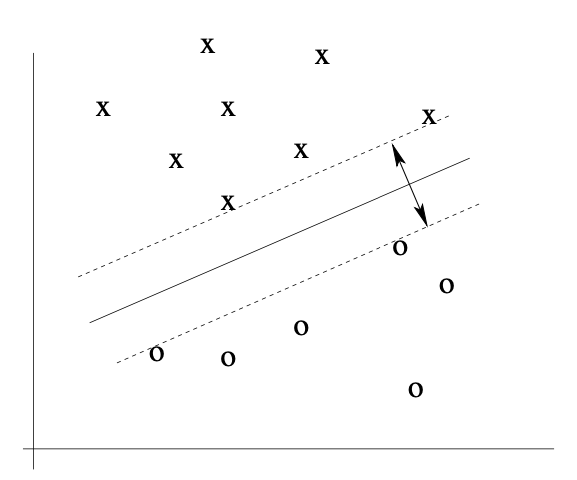
\includegraphics[width=0.5\textwidth]{Images/6.png}
    \caption{Margen de un clasificador lineal: las cruces representan puntos de entrenamiento con 
    etiqueta \(+1\), mientras que los círculos representan puntos de entrenamiento con etiqueta \(-1\). 
    La línea recta es el clasificador lineal \(f_n\), y la línea discontinua muestra el margen. La 
    anchura \(\rho\) del margen está representada por la flecha.(Gráfica tomada de [1])}
    \label{fig:Clasificación con margen}
\end{figure}

Se puede demostrar que la dimensión VC de la clase \(\mathcal{F}_\rho\) de funciones lineales con 
margen al menos \(\rho\) puede ser acotada esencialmente por la razón entre el radio \(R\) de la 
esfera más pequeña que encierra los puntos de datos y el margen \(\rho\), es decir,

\[
\text{VC}(\mathcal{F}_\rho) \leq \min \left\{d, \frac{4R^2}{\rho^2} \right\} +1.
\]

(cf. Teorema 5.1 en Vapnik, 1995). Es decir, cuanto mayor sea el margen \(\rho\) de las funciones 
en la clase \(\mathcal{F}_\rho\), menor será su dimensión VC. De esta manera, se puede usar el 
margen de los clasificadores como un concepto de capacidad. Uno de los clasificadores más conocidos, 
la \textbf{máquina de soporte vectorial} (SVM, \textit{Support Vector Machine}), se basa en este 
resultado. Para un tratamiento más completo, véase Schölkopf y Smola (2002).\newline

Un ejemplo de cota de generalización que involucra el gran margen es el siguiente (para una 
declaración más precisa, véase el Teorema 7.3 en Schölkopf y Smola, 2002):\newline

\begin{thm}[Cotas de grandes márgenes]

Supongamos que el espacio de datos está contenido dentro de una esfera de radio \(R\) en 
\(\mathbb{R}^d\). Consideremos el conjunto \(\mathcal{F}_\rho\) de clasificadores lineales con 
margen al menos \(\rho\). Supongamos que se nos dan \(n\) ejemplos de entrenamiento. Denotemos 
por \(\nu(f)\) la fracción de ejemplos de entrenamiento con margen menor que \(\rho\) o que han 
sido clasificados erróneamente por algún clasificador \(f \in \mathcal{F}_\rho\). Entonces, con 
probabilidad al menos \(1 - \delta\), el error verdadero de cualquier \(f \in \mathcal{F}_\rho\) 
puede ser acotado por:

\[
\mathcal{R}(f) \leq \nu(f) + \sqrt{\frac{c}{n} \left( \frac{R^2}{\rho^2} \log(n)^2 + \log(1/\delta) \right)} .
\]
\end{thm}

\subsection{Conclusiones acerca de las cotas de generalización}

Hasta ahora, hemos introducido algunos conceptos de capacidad para clases de funciones: el 
coeficiente de fragmentación, la dimensión VC y la complejidad de Rademacher. En la literatura, 
existen muchos otros conceptos de capacidad, y presentarlos todos está fuera del alcance de esta 
visión general. Sin embargo, queremos destacar la forma general que suelen adoptar la mayoría 
de las cotas de generalización.\newline

Usualmente, estas cotas están compuestas por tres términos diferentes y tienen la siguiente forma: 
con probabilidad al menos \(1 - \delta\),

\[
\mathcal{R}(f) \leq R_{\text{emp}}(f) + \text{capacidad}(\mathcal{F}) + \text{confianza}(\delta).
\]

Es decir, se puede acotar el riesgo verdadero de un clasificador por su riesgo empírico, un término 
de capacidad que, en el caso más simple, solo depende de la clase de funciones subyacente 
\(\mathcal{F}\), y un término de confianza que depende de la probabilidad con la que se desea que 
la cota se cumpla.\newline

Nótese que, por su naturaleza, todas las cotas de esta forma son cotas en el peor caso: dado que 
la cota se cumple para todas las funciones en la clase \(\mathcal{F}\), el comportamiento de la cota 
está determinado por el peor clasificador dentro del espacio funcional. Este punto suele ser 
utilizado para criticar este enfoque en la teoría del aprendizaje estadístico, ya que los clasificadores 
naturales no tienden a seleccionar la peor función dentro de una clase.\newline


\section{Consistencia de Bayes y error de aproximación}

Hasta ahora, hemos reparado tan solo en el enfoque estándar para acotar el error de estimación 
de un clasificador. Esto es suficiente para lograr consistencia con respecto a una clase de funciones 
dada \(\mathcal{F}\). En esta sección, queremos analizar la pieza faltante para lograr la 
\textbf{consistencia de Bayes}: el error de aproximación.\newline

Recordemos que el error de estimación se definía como \(\mathcal{R}(f_n) - \mathcal{R}(f_{\mathcal{F}})\) 
y el error de aproximación como \(\mathcal{R}(f_{\mathcal{F}}) - \mathcal{R}(f_{\text{Bayes}})\) 
(\ref{def:consistencias}). Para lograr consistencia de Bayes, ambos términos deben tender a cero cuando 
\(n \to \infty\). Hemos visto que, para que el error de estimación converja a \(0\), debemos 
asegurarnos de que el espacio funcional \(\mathcal{F}\) tenga una capacidad razonablemente baja.\newline

Sin embargo, esto plantea un problema para el error de aproximación: si el espacio funcional 
\(\mathcal{F}\) tiene una capacidad pequeña, esto significa, en particular, que el espacio 
\(\mathcal{F}\) es considerablemente más pequeño que el espacio de todas las funciones posibles 
\(\mathcal{F}_{\text{all}}\). Por lo tanto, si fijamos la clase de funciones \(\mathcal{F}\) y 
\(f_{\text{Bayes}}\) no está contenido en \(\mathcal{F}\), entonces el 
error de aproximación podría no ser cero.\newline

Existen solo dos formas de resolver este problema. La primera es imponer condiciones sobre la 
forma funcional del clasificador de Bayes. Si \(f_{\text{Bayes}} \in \mathcal{F}\) para algún 
espacio funcional conocido \(\mathcal{F}\) con capacidad pequeña, entonces sabemos que el error 
de aproximación es \(0\). En este caso, la consistencia de Bayes se reduce a la consistencia con 
respecto a \(\mathcal{F}\), lo cual puede lograrse mediante los métodos discutidos previamente. 
Sin embargo, si no queremos hacer suposiciones sobre el clasificador de Bayes, entonces 
debemos optar por una enfoque diferente.\newline

\subsection{Espacios funcionales anidados}

En esta construcción, no consideraremos una única clase de funciones \(\mathcal{F}\), sino una 
secuencia de espacios funcionales \(\mathcal{F}_1, \mathcal{F}_2, \dots\). Al construir un 
clasificador sobre \(n\) puntos de datos, lo haremos a partir del espacio funcional \(\mathcal{F}_n\). 
La clave de esta construcción es que el espacio funcional \(\mathcal{F}_n\) debe volverse más 
complejo a medida que el tamaño de la muestra \(n\) aumenta.\newline

El enfoque estándar es elegir los espacios \(\mathcal{F}_n\) de modo que formen una secuencia 
creciente de espacios funcionales anidados, es decir,

\[
\mathcal{F}_1 \subset \mathcal{F}_2 \subset \mathcal{F}_3 \subset \dots
\]

La intuición detrás de esto es que comenzamos con un espacio funcional simple y luego, 
gradualmente, agregamos funciones más complejas al espacio. Si ahora se nos da una muestra 
de \(n\) puntos de datos, seleccionamos nuestro clasificador del espacio \(\mathcal{F}_n\). 
Para que este clasificador sea consistente con Bayes, debemos garantizar dos condiciones:\newline

\begin{enumerate}
    \item \textbf{El error de estimación debe converger a 0 cuando \(n \to \infty\).} Para lograr esto, 
    notemos que para cada \(n\) fijo, podemos acotar el error de estimación utilizando uno de los 
    métodos conocidos. Esta cota disminuye conforme aumenta el tamaño de la muestra, pero 
    crece cuando el término de complejidad aumenta. Debemos entonces asegurarnos de que el error de 
    estimación total decrezca de forma neta, es decir, que el término de complejidad no domine al término 
    del tamaño de la muestra. Para garantizar esto, debemos asegurarnos de que la complejidad de 
    \(\mathcal{F}_n\) no crezca demasiado rápido a medida que aumenta \(n\).

    \item \textbf{El error de aproximación debe converger a 0 cuando \(n \to \infty\).} Intuimos que 
    para lograrlo, 
    debiéramos garantizar que, eventualmente, para algún \(n\) suficientemente grande, cada función en 
    \(\mathcal{F}_{\text{all}}\) esté contenida en \(\mathcal{F}_n\), o que pueda ser aproximada por 
    una función en \(\mathcal{F}_n\). Discutiremos a continuación cómo puede lograrse.
\end{enumerate}


Un ejemplo de cómo estas dos condiciones pueden formularse de manera rigurosa se presenta en el 
siguiente teorema, adaptado del Teorema 18.1 de Devroye et al. (1996):\newline

\begin{thm}
 Sea \(\mathcal{F}_1, \mathcal{F}_2, \dots\) una secuencia de espacios funcionales, y 
consideremos los clasificadores 

\[
f_n = \arg\min_{f \in \mathcal{F}_n} R_{\text{emp}}(f).
\]

Supongamos que, para cualquier distribución \(P\), se satisfacen las siguientes dos condiciones:

\begin{enumerate}
    \item Las dimensiones VC de los espacios \(\mathcal{F}_n\) satisfacen 
    \[
    \text{VC}(\mathcal{F}_n) \cdot \log n / n \to 0
    \]
    cuando \(n \to \infty\).
    
    \item El error de aproximación satisface \(\mathcal{R}(f_{\mathcal{F}_n}) \to \mathcal{R}(f_{\text{Bayes}})\) 
    cuando \(n \to \infty\).
\end{enumerate}

Entonces, la secuencia de clasificadores \(f_n\) es consistente con Bayes.

\end{thm}
\vspace{0.3cm}

Intentemos entender este teorema. Se nos da una secuencia creciente de espacios funcionales \(\mathcal{F}_n\). 
Para cada muestra de tamaño \(n\), elegimos la función en \(\mathcal{F}_n\) que minimiza el riesgo empírico. 
Este es nuestro clasificador \(f_n\). Si queremos que este clasificador sea consistente, deben cumplirse dos 
condiciones.\newline

La primera condición establece que la complejidad de las clases de funciones, medida mediante la dimensión VC, 
debe crecer lentamente. Por ejemplo, si elegimos los espacios funcionales \(\mathcal{F}_n\) de modo que 
\(\text{VC}(\mathcal{F}_n) \approx n^\alpha\) para algún \(\alpha \in (0,1)\), entonces la primera condición 
se satisface porque

\[
\text{VC}(\mathcal{F}_n) \cdot \frac{\log n}{n} \approx n^\alpha \cdot \frac{\log n}{n} = \frac{\log n}{n^{1-\alpha}} \to 0.
\]

Sin embargo, si elegimos \(\text{VC}(\mathcal{F}_n) \approx n\) (es decir, \(\alpha = 1\) en el cálculo anterior), 
entonces la condición ya no se cumple:

\[
\text{VC}(\mathcal{F}_n) \cdot \frac{\log n}{n} \approx \log n \to \infty.
\]

La segunda condición del teorema simplemente establece que el error de aproximación debe converger a \(0\), pero 
el teorema no proporciona información sobre cómo lograr esto. Sin embargo, como discutimos anteriormente, es claro 
que esto solo se puede alcanzar mediante una secuencia creciente de clases de funciones.\newline

\subsection{Regularización}

Una forma implícita de trabajar con espacios funcionales anidados es el \textbf{principio de regularización}. 
En lugar de minimizar el riesgo empírico \(R_{\text{emp}}(f)\) y luego expresar la capacidad de generalización 
del clasificador resultante \(f_n\) mediante alguna medida de capacidad de la clase funcional subyacente 
\(\mathcal{F}\), se puede seguir un enfoque más directo: se minimiza directamente el llamado \textbf{riesgo 
regularizado}:

\[
\mathcal{R}_{\text{reg}}(f) = R_{\text{emp}}(f) + \lambda \Omega(f).
\]

Aquí, \(\Omega(f)\) es el llamado \textbf{regularizador}. Este regularizador está diseñado para penalizar 
funciones excesivamente complejas. Por ejemplo, a menudo se elige un regularizador que penaliza funciones con 
grandes fluctuaciones, es decir, se elige \(\Omega(f)\) de modo que sea pequeño para funciones que varían 
lentamente y grande para funciones que fluctúan mucho. Como otro ejemplo, en clasificadores lineales se puede 
elegir \(\Omega(f)\) como el inverso del margen de una función (definición \ref{def:margen}).\newline

El parámetro \(\lambda\) en la definición del riesgo regularizado es una constante de ajuste que equilibra la 
importancia de \(R_{\text{emp}}(f)\) y \(\Omega(f)\). Si \(\lambda\) es muy grande, tomamos la penalización 
inducida por \(\Omega(f)\) muy seriamente y podríamos preferir funciones con \(\Omega(f)\) pequeño, incluso si 
tienen un alto riesgo empírico. Por otro lado, si \(\lambda\) es pequeño, la influencia de la penalización 
disminuye y simplemente elegimos funciones basándonos en sus riesgos empíricos.\newline

El principio de regularización consiste en elegir el clasificador \(f_n\) que minimiza el riesgo regularizado 
\(\mathcal{R}_{\text{reg}}(f)\). Muchos de los clasificadores ampliamente utilizados pueden formularse dentro 
del marco de la regularización, por ejemplo, la máquina de soporte vectorial (conocidas como SVM o Support Vector Machines)
(ver Schölkopf y Smola, 2002, 
para más detalles).\newline

Para demostrar la \textbf{consistencia de Bayes} de clasificadores regularizados, se procede esencialmente como 
se describió en la subsección anterior: para alguna secuencia lentamente creciente \(\omega_1, \omega_2, \dots\), 
consideramos espacios funcionales anidados \(\mathcal{F}_{\omega_1}, \mathcal{F}_{\omega_2}, \dots\), donde cada 
\(\mathcal{F}_{\omega_i}\) contiene todas las funciones \(f\) que satisfacen \(\Omega(f) \leq \omega_i\). 
Eventualmente, si \(i\) es lo suficientemente grande, el espacio \(\mathcal{F}_{\omega_i}\) aproximará el 
espacio \(\mathcal{F}_{\text{all}}\) de todas las funciones.\newline

Para garantizar la consistencia, se debe hacer que la constante \(\lambda\) tienda a \(0\) cuando \(n \to \infty\). 
Esto asegura que, para \(n\) grande, efectivamente se nos permita elegir funciones de un espacio cercano a 
\(\mathcal{F}_{\text{all}}\). Por otro lado, la constante \(\lambda\) no debe converger a \(0\) demasiado rápido, 
ya que, de lo contrario, comenzaríamos a sobreajustar para valores pequeños de \(n\) (si \(\lambda\) es muy 
pequeño, esencialmente se ignora el regularizador y, en consecuencia, se realiza algo similar a la minimización
de riesgo empírico pero sobre un conjunto muy grande de funciones).\newline

Nótese que existe una diferencia conceptual importante entre la minimización del riesgo empírico y la 
regularización. En la regularización, se introduce una función \(\Omega\) que mide la \textbf{complejidad} de 
una función individual \(f\). En ERM, por otro lado, nunca observamos la complejidad de funciones individuales, 
sino solo la complejidad de una clase funcional completa. Esta última, sin embargo, es más bien una medida de 
\textbf{capacidad}, es decir, una medida de la cantidad de funciones en \(\mathcal{F}\), y solo indirectamente 
una medida de qué tan complejas son las funciones individuales en la clase. Desde un punto de vista intuitivo, 
el primer enfoque es a menudo más fácil de comprender, ya que la complejidad de una función individual es un 
concepto más tangible que la capacidad de una clase funcional completa.\newline

El teorema anterior muestra el principio general de cómo podemos lograr la \textbf{consistencia de Bayes}. 
Sin embargo, el teorema simplemente establece como su segunda condición que el error de aproximación 
debe converger a \(0\). ¿Cómo se puede lograr esto en la práctica? Resulta que hay muchas situaciones 
en las que esto no es tan difícil. Esencialmente, debemos asegurarnos de que cada función en 
\(\mathcal{F}_{\text{all}}\) esté contenida en \(\mathcal{F}_n\) para algún \(n\) grande, o que pueda 
ser aproximada arbitrariamente bien por una función de \(\mathcal{F}_n\).\newline

El área de las matemáticas que estudia este tipo de problemas se llama \textbf{teoría de la aproximación}, 
pero para los propósitos de la teoría del aprendizaje, resultados de aproximación simples suelen ser 
suficientes. El único 
problema técnico que debemos resolver es obtener una afirmación de la siguiente forma: si dos funciones 
son cercanas entre sí, entonces sus valores de riesgo también son cercanos.

Afirmaciones de este tipo suelen ser bastante fáciles de obtener. Por ejemplo, es directo ver que si 
\(f\) es una función de clasificación binaria (es decir, con \(f(x) \in \{\pm1\}\)) y \(g\) es cualquier 
otra función medible arbitraria, y la distancia \(L_1\) entre \(f\) y \(g\) es menor que \(\delta\), 
entonces su diferencia en el riesgo 0-1 también es menor que \(\delta\), es decir,

\[
P(f(x) \neq \text{sgn}(g(x))) < \delta.
\]

Esto significa que, para demostrar que el error de aproximación de un espacio funcional \(\mathcal{F}\) 
es menor que \(\delta\), solo necesitamos saber que cada función en \(\mathcal{F}_{\text{all}}\) puede 
ser aproximada hasta \(\delta\) en la norma \(L_1\) por funciones de \(\mathcal{F}\).\newline

Resultados de este tipo son abundantes en la literatura matemática. Por ejemplo, si \(\mathcal{X}\) es un subconjunto 
acotado de los números reales, es bien sabido que se puede aproximar cualquier función medible sobre este 
conjunto de manera arbitrariamente precisa mediante un polinomio. Por lo tanto, podríamos elegir los espacios 
\(\mathcal{F}_n\) como los espacios de polinomios de grado a lo sumo \(d_n\), donde \(d_n\) crece lentamente 
con \(n\). Esto es suficiente para garantizar la convergencia del error de aproximación.\newline

\section{Los teoremas de la chancha y los veinte}

Hemos presentado, además de parte de la historia de la disciplina, algunos resultados positivos en la teoría del aprendizaje estadístico. 
Formalizamos el problema de aprendizaje, hemos definido el objetivo del aprendizaje -minimizar el 
riesgo-, hemos especificado qué propiedades debe tener un clasificador -hablamos de la consistencia- y también hemos desarrollado un 
marco para pensar estas propiedades de manera fundamental. Además, vimos que existen 
diferentes formas de lograr clasificadores consistentes, de las cuales hemos mencionado algunas (como los \(k\)-vecinos más cercanos y la 
minimización del riesgo empírico).\newline

Ahora surge de manera natural la siguiente pregunta: ¿cuál de todos los clasificadores consistentes 
es \textit{el mejor} clasificador? ¿Existe un clasificador universalmente bueno?\newline

Intentemos reformular esta pregunta de una manera más formal. Manteniendo la restricción de muestreo iid
a partir de alguna distribución de probabilidad subyacente pero desconocida, ¿existe 
un clasificador que, en promedio sobre todas las distribuciones de probabilidad, obtenga mejores 
resultados que cualquier otro clasificador? ¿Podemos comparar dos clasificadores \(f\) y \(g\), 
en promedio sobre todas las distribuciones?\newline

La razón por la cual consideramos afirmaciones ``en promedio sobre todas las distribuciones'' radica 
en que no queremos hacer ninguna suposición sobre la distribución subyacente. Por lo tanto, parece 
natural estudiar el comportamiento de los clasificadores en cualquier posible distribución. Veamos entonces
que, no solamente no existe un clasificador universalmente bueno, sino que, en promedio sobre todas las distribuciones
posibles, todos los clasificadores son equivalentes.\newline

Para tener alguna intuición al respecto, supongamos que nuestro espacio de entrada \(\mathcal{X}\) solo consiste en un conjunto finito de puntos, es decir, 
\(X = \{x_1, \dots, x_m\}\) para algún número grande \(m\). Ahora consideremos todas las formas 
posibles de asignar etiquetas a esos puntos de datos, es decir, consideremos todas las distribuciones 
de probabilidad posibles sobre \(\mathcal{X}\). \newline

Dado un pequeño subconjunto de puntos de entrenamiento \((X_i, Y_i)_{i=1,\dots,n}\), con $n<m$, utilizamos 
alguna regla de clasificación para construir un clasificador a partir de esos puntos. Es decir, fijamos un clasificador $f$
construido con $n$ puntos etiquetados del espacio finito \(\mathcal{X}\).\newline

Ahora, consideremos todos los puntos de \(\mathcal{X}\) que no han sido usados como 
puntos de entrenamiento y sus etiquetas. Solemos llamar conjunto de prueba (\textit{test set}) a este conjunto.
Por un lado, existe una asignación de etiquetas posible \(P_1\) sobre el conjunto de prueba (los datos que el clasificador
no conoce) en la que el 
clasificador no comete ningún error, específicamente aquella que coincide exactamente con la asignación 
de etiquetas producida por el clasificador mismo. Sin embargo, también existe una asignación de 
etiquetas \(P_2\) en la que el clasificador comete el mayor error posible: basta tomar la distribución
que asigna a los datos de prueba etiquetas de forma inversa a la del clasificador. \newline

De la misma manera, podemos ver que, esencialmente, para cualquier error \(R\) dado, podemos 
construir una distribución de probabilidad sobre \(\mathcal{X}\) tal que el error del clasificador \(f_n\) en el 
conjunto de prueba sea exactamente \(R\). El mismo razonamiento se aplica a cualquier otro 
clasificador. Por lo tanto, si promediamos sobre todas las distribuciones de probabilidad posibles en \(\mathcal{X}\), 
todos los clasificadores \(f_n\) alcanzarán el mismo error de prueba: cada vez que existe una 
distribución en la que el clasificador obtiene un buen rendimiento, existe una distribución 
(digamos) opuesta sobre el conjunto de prueba en la que el clasificador obtiene un mal rendimiento.
En particular, en promedio sobre todas las distribuciones de probabilidad, ningún 
clasificador puede ser mejor que un clasificador aleatorio en el conjunto de prueba.\newline

Si bien este resultado pareciera atacar las mismas bases de la teoría del aprendizaje estadítico que nos hemos esmerado en 
construir, en realidad es algo bastante esperable cuando reparamos en el hecho de que estamos planteando
medir la capacidad de un clasificador cualquiera sobre \textit{todas} las distribuciones posibles. Como a priori
no imponemos condiciones de ningún tipo sobre la distribución de probilidad, dado un clasificador cualquiera construido
en base a $n$ puntos, siempre podríamos hallar una distribución -al menos teórica- sobre la que dicho clasificador no tenga
manera de generalizar los aprendido. Por ejemplo, se puede construir una distribución de probabilidad sobre las etiquetas simplemente 
lanzando una moneda y, para cada punto de datos, decidir su etiqueta verdadera según el resultado del 
lanzamiento aleatorio. \newline

Parece plausible que, en un escenario así, no sirva de nada conocer las etiquetas de los puntos de 
entrenamiento. La única manera de aprender es excluir tales casos artificiales. Necesitamos asegurarnos 
de que existe algún mecanismo inherente por el cual podamos usar las etiquetas de entrenamiento para 
generalizar exitosamente a las etiquetas de prueba. Formalmente, esto significa que debemos restringir 
el espacio de distribuciones de probabilidad bajo consideración. Es decir, no podemos partir sin asumir
nada acerca de la distribución.\\

En inglés, se utiliza la expresión \textit{no free lunch} para hacer referencia
a situaciones donde es necesario hacer compromisos y ceder, y de ahí deriva el nombre de los varios teoremas
que formalizan la problemática de esta sección. En un intento de hacernos propio el tema, los llamaremos 
telúricamente, \textit{los teoremas de la chancha y los veinte}. 
A continuación, enunciamos y probamos uno de los teoremas mencionados, resultado de Devroye en 1982, que encuadra la
situación desde la perspectiva de la convergencia del riesgo.\newline


\begin{thm}[de la chancha y los veinte]
Sea \(\varepsilon > 0\). Para cualquier entero \(n\) y cualquier 
regla de clasificación \(f_n\), existe una distribución \(P(X, Y)\) con riesgo bayesiano 
\(\mathcal{R}(f_{Bayes}) = 0\) tal que:

\[
\mathbb{E}[\ell(X,Y,f_n)] \geq \frac{1}{2} - \varepsilon.\newline
\]
\end{thm}

\begin{proof}

Construiremos una familia de distribuciones conjuntas para el par de variables aleatorias \((X, Y)\) y mostraremos que para al menos un 
elemento de esta familia, cualquier clasificador \(f_n\) -construido en base a $n$ puntos en $X$-, presenta un rendimiento deficiente.\newline

Consideremos un espacio de entrada 
discreto \(\mathcal{X}\) que se distribuye uniformemente sobre el conjunto finito \(\{1, 2, \dots, K\}\), 
según la función distribución de probabilidad discreta:

\[
P(X = i) = \begin{cases} 
\frac{1}{K}, & \text{si } i \in \{1, 2, \dots, K\}, \\ 
0, & \text{en otro caso}.
\end{cases}
\]


Construida la distribución de \(\mathcal{X}\), definamos la distribución conjunta \(P(X,Y)\). Como \(\mathcal{X}\) es finita,
es posible parametrizar la distribución conjunta con un solo valor
\(b \in [0,1)\). Luego, cada distribución posible de $(X,Y)$ puede es representada por un único valor \(b\).
Tomando la expansión binaria de $b$, tenemos:

\[
b = 0.b_0 b_1 b_2 \dots.
\]

Definimos entonces la etiqueta \(Y\) como función de \(X\):

\[
Y = b_X,
\]

donde \(b_X\) coincide con el \(X\)-ésimo dígito binario de \(b\). Utilizar la expansión binaria de $b$ facilita la interpretación
de la parametrización, dado que cada dígito $i$-ésimo es exactamente la etiqueta correspondiente a la muestra $i$-ésima.
Por ejemplo, si \(K=3\) y estamos en el caso donde  \(f_{Bayes}(X_1)=0\),  \(f_{Bayes}(X_2)=1\) y \(f_{Bayes}(X_3)=1\), 
la distribucíon conjunta estaría representada por $b=0,011$.\newline


Dado que \(Y\) es una función de \(X\), existe una regla de decisión perfecta y el clasificador de Bayes alcanza una pérdida cero:

\[
\ell(X,Y,f_{Bayes}) = 0.
\]

Consideramos a $f_n$ un clasificador sobre $X$ construido a partir de las primeras $n$ muestras. Escribimos entonces
\[
f_n(X) = f_n(X, Z_n),
\]
para explicitar que $f_n$ es función también de la muestra de entrenamiento $Z_n$. Luego, definimos el riesgo sobre \(b\)
como el riesgo de $f_n$ para esa distribución asociado a la pérdida-0-1:


\begin{equation*}
    \begin{aligned}
        \mathcal{R}_n(b) &= \mathbb{E}[\ell((X,Y)(b),f_n(X))]\\ 
        &= \sum_{i=1}^{K} 1 \cdot P(f_n(X_i, Z_n) \neq b_{i}) + \sum_{i=1}^{K} 0 \cdot P(f_n(X_i, Z_n) = b_{i})\\
        &= \sum_{i=1}^{K} P(f_n(X_i, Z_n) \neq b_{i}) \\
        &= P(f_n(X, Z_n) \neq Y).
    \end{aligned}
\end{equation*}


Ahora introducimos una variable aleatoria \(B\), distribuida uniformemente en \([0,1)\) e independiente de \(X\) y 
de los datos de entrenamiento \(Z_n\). Su expansión binaria es: \(B = 0,B_1B_2B_3\dots\), que es una sucesión 
de variables aleatorias independientes en \(\{0,1\}\) con probabilidad $\frac{1}{2}$. Evidentemente, el rol de $B$
es generar una distribución conjunta sobre $X$ e $Y$ de manera aleatoria. También podemos generar de manera aleatoria
una distribución para $Y$, que podemos llamar $Y=B_X$, usando la misma convención que antes donde, de nuevo,
$B_X$ es el dígito que corresponde al punto $X$ en la expansión binaria de $B$. Notemos que $X$ puede no pertenecer
al conjunto de entrenamiento $Z_n$. \newline
Podemos expresar el riesgo de este nuevo parámetro como:


\[
\mathcal{R}_n(B) = P(f_n(X, Z_n) \neq B_X).\newline
\]

y dado que $B$ representa a cualquiera de las distribuciones parametrizadas por $b$, es cierto que

\begin{equation}
    \sup_{b\in[0,1)} \mathcal{R}_n(b) \geq \mathcal{R}_n(B). \label{eq:cota_parametro_b_distribuciones}
\end{equation}



Notemos que \(B_X\) es una variable de Bernoulli(\(1/2\)) independiente de \(f_n(X, Z_n)\) cuando 
\(X\) no pertenece al conjunto de entrenamiento. De aquí se obtiene:

\[
P(f_n(X, Z_n) \neq B_X \mid X, Z_n) = \frac{1}{2}, \quad \text{si } X \notin \{X_1, \dots, X_n\}.
\]

Esto se debe a que el clasificador no tiene información sobre la etiqueta de \(X\) si \(X\) no está en el conjunto de entrenamiento,
como es el caso y, dado que $B_X$ se genera aleatoriamente, la probabilidad de que $f_n$ acierte es de $1/2$. \newline

Esto nos sirve para
dar la siguiente expresión del riesgo de $B$:\newline
\begin{equation*}
    \begin{aligned}
        \mathcal{R}_n(B) &= P(f_n(X, Z_n) \neq B_X)\\
        &= P(f_n(X, Z_n) \neq B_X \mid X \notin \{X_1, \dots, X_n\}) \cdot P(X \notin \{X_1, \dots, X_n\})\\
        &  \qquad + P(f_n(X, Z_n) \neq B_X \mid X \in \{X_1, \dots, X_n\}) \cdot P(X \in \{X_1, \dots, X_n\})\\
        &\geq P(f_n(X, Z_n) \neq B_X \mid X \notin \{X_1, \dots, X_n\}) \cdot P(X \notin \{X_1, \dots, X_n\})\\
        & = \frac{1}{2} \cdot P(X \notin \{X_1, \dots, X_n\})
    \end{aligned}
\end{equation*}

Donde simplemente separamos los eventos en donde el punto $X$ sobre el que analizamos al clasificador está o no está
en el conjunto de entrenamiento, y desechamos el caso afirmativo. Luego

\[
\mathcal{R}_n(B) = P(f_n(X, Z_n) \neq B_X) \geq \frac{1}{2} \cdot P(X \notin \{X_1, \dots, X_n\})
\]

Por otro lado, como las muestras son tomadas de forma iid:
\[
\begin{aligned}
    P(X \notin \{X_1, \dots, X_n\}) &= P(X\neq X_1, X\neq X_2, \dots, X\neq X_n) \\
   &= P(X\neq X_1)^n \\
   &= \left(1-\frac{1}{K}\right)^n
\end{aligned}
\]

Luego

\[
\mathcal{R}_n(B) \geq \frac{1}{2} \cdot \left(1-\frac{1}{K}\right)^n
\]

Considerando la cota \ref{eq:cota_parametro_b_distribuciones}, sabemos que existe una distribución
conjunta $(X,Y)(b)$ tal que 

\[
\mathcal{R}_n(b) \; =\; \mathbb{E}[\ell((X,Y)(b),f_n(X))] \; \geq \;  \frac{1}{2} \cdot \left(1-\frac{1}{K}\right)^n \xrightarrow[K \to \infty]{} \frac{1}{2}
\]


\end{proof}

Este teorema establece que, aunque existen reglas de clasificación que son universalmente 
consistentes, es decir, que asintóticamente proporcionan el rendimiento óptimo para cualquier 
distribución, su desempeño en muestras finitas siempre será muy malo -cercano al de clasificar utilizando el lanzamiento de una moneda- para algunas 
distribuciones. \newline

Esto significa que ningún clasificador puede garantizar que logremos un error aceptable 
para todas las distribuciones, aún teniendo una cantidad de muestras enorme (pero finita). 
Sin embargo, dado que la distribución adversa depende de \(n\), 
el Teorema no nos permite concluir que existe una única distribución para la cual la 
probabilidad de error sea mayor que, por ejemplo, \(\ell(f_{Bayes}) + 1/4\) para todo \(n\). Tal afirmación 
iría en contradicción la propia existencia de reglas universalmente consistentes. \newline


Las restricciones sobre la distribución de probabilidad pueden adoptar diversas formas. Podríamos suponer que la distribución 
subyacente tiene una función de densidad que \textit{se comporta bien}. O
que existe una función de distancia en el espacio de entrada y que las etiquetas dependen de alguna manera 
continua de la distancia, es decir, que los puntos cercanos tienden a tener etiquetas similares. Si 
hacemos tales suposiciones, es posible construir clasificadores que las exploten (por ejemplo, el clasificador 
\(k\)-NN para aprovechar la estructura de distancia). Desde ya que el teorema sigue siendo válido, lo que significa que habrá conjuntos de datos 
para los cuales este clasificador fallará estrepitosamente. Sin embargo, estos serán conjuntos de datos 
provenientes de distribuciones donde las suposiciones han sido gravemente violadas. Y en tales casos, tiene 
sentido que un clasificador que se basa en esas suposiciones no tenga ninguna posibilidad de éxito.

\begin{figure}[ht!]
    \centering
    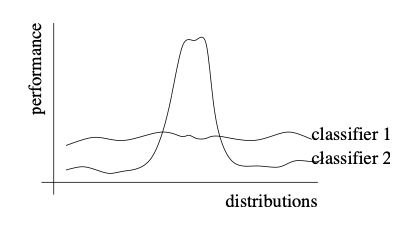
\includegraphics[width=0.5\textwidth]{Images/7.png}
    \caption{Tomando en consideración todas las distribuciones posibles -eje X-, el clasificador 1
    es en general mejor que el clasificador 2, y este último es muchísimo mejor para un subconjunto
    de distribuciones. Podemos pensar que 1 es un clasificador general y 2 está construído para un tipo
    de problemas específico. El teorema de la chancha y los veinte nos dice que el área debajo de ambas
    curvas debe ser igual, es decir que en promedio ambos clasificadores tienen el mismo error. (Gráfica tomada de [1])}
    \label{fig:no_free_lunch_theorem}
\end{figure}

Un problema que suele surgir en el contexto del teorema de la chancha y los veinte es cómo se relaciona con los 
teoremas de consistencia demostrados anteriormente. Por ejemplo, vimos que el clasificador 
de los \(k\)-vecinos más cercanos es universalmente consistente, es decir, es consistente para cualquier 
distribución subyacente \(P\). La solución a esta aparente paradoja radica en el hecho de que las afirmaciones de consistencia solo tratan 
el caso límite cuando \(n \to \infty\). En el ejemplo del espacio de datos finito mencionado anteriormente, 
notemos que, tan pronto como el tamaño de la muestra es lo suficientemente grande como para haber muestreado 
esencialmente cada zona del espacio al menos una vez, un clasificador que memoriza los datos de entrenamiento 
ya no cometerá más errores. Afirmaciones similares (aunque algo más complicadas) también son válidas en casos 
de espacios de datos infinitos. Así, los teoremas de la chancha y los veinte hacen afirmaciones sobre un tamaño de muestra finito \(n\), mientras que 
la consistencia considera el límite cuando \(n \to \infty\).\newline

Otra manera de expresar esto es la siguiente: si las etiquetas de los puntos se asignan de manera 
completamente aleatoria, entonces las etiquetas de los puntos de prueba serán completamente independientes 
de las etiquetas de los puntos de entrenamiento. En tal escenario, el aprendizaje es imposible.\newline



\chapter*{Bibliografía}

[1] von Luxburg, B. Schölkopf - \textit{Statistical Learning Theory: Models, Concepts and Results} (2008). \\

[2] Vladimir Vapnik - \textit{The Nature of Statistical Learning Theory} (1995). \\

[3] Vladimir Vapnik  - \textit{Statistical Learning Theory} (1998). \\

[4] Luc Devroye, László Györfi, Gábor Lugosi - \textit{A Probabilistic Theory of Pattern Recognition} (1996). \\

[5] B. Schölkopf, A. Smola - \textit{Learning with Kernels} (1996). \\

[6] G. Casella, R. Berger \textit{Statistical Inference, Second Edition} (2002). \\

[7] C. Bishop - \textit{Pattern Recognition and Machine Learning} (2006). \\

[8] V. N. Vapnik, A. YA. Chervonenkis - \textit{On the uniform convergence of relative frequencies of events to their probabilities} (1971)\\

[9] A. YA. Khinchin -  \textit{On basic theorems of information theory} (1956), pp. 17-75.\\

[10] W. Feller - \textit{Introduction to Probability Theory and its Applications, Vol. 1}  (1957).\\

[11] Abu-Mostafa et al - \textit{Learning From Data} (2012)




\end{document}